% import gaya yang sudah disiapkan
\documentclass{gaya}

% import berbagai variabel
\titleind{Evaluasi Performa Hadoop dan Spark pada DigitalOcean menggunakan HiBench dalam Konfigurasi \textit{Pseudo Distributed}} % yang ini untuk di cover
\titleindinline{Evaluasi Performa Hadoop dan Spark pada DigitalOcean menggunakan HiBench dalam Konfigurasi \textit{Pseudo Distributed}} % yang ini untuk di dalam paragraf
\titleen{Performance Evaluation of Hadoop and Spark on DigitalOcean using HiBench in a Pseudo-Distributed Configuration}

\fullname{Dimas Wahyu Saputro} % diisi nama Anda
\newcommand{\fullnamenc}{Dimas Wahyu Saputro} % diisi nama Anda
\idnum{120450081} % diisi NIM Anda

\approvaldate{31 Mei 2024} % diisi tanggal penulisan
\newcommand{\approvaldatenc}{31 Mei 2024}

\degre{Sarjana Sains Data}
\yearsubmit{2024} % diisi tahun penulisan
\program{Sains Data} % prodi
\dept{Sains} % fakultas

\firstsupervisor{Tirta Setiawan, S.Pd., M.Si.} % nama pembimbing 1
\nipnrkfirst{NIP. } % diisi NIP atau NRK
\firstnip{199008222022031003}

\secondsupervisor{Riksa Meidy Karim, S.Kom., M.Si., M.Sc.} % nama pembimbing 2
\nipnrksecond{ }
\secondnip{ }

\headofdepartment{Tirta Setiawan, S.Pd., M.Si.} % nama koordinator prodi
\nipnrkhead{NIP. }
\headnip{199102302020012003}

\def\tahapan{sidang} % opsi: sempro, semhas, sidang, atau final

%-----------------------------------------------
% Input tahapan Tugas akhir Anda saat ini
%-----------------------------------------------
% diisi dengan:
% sempro (jika dibuat untuk seminar proposal),
% semhas (jika untuk seminar hasil),
% sidang (untuk sidang), atau
% final (jika sudah final dan siap cetak)

\def\sempro{sempro}
\def\semhas{semhas}
\def\sidang{sidang}
\def\final{final}

\ifx\tahapan\sempro
\textta{Proposal Skripsi}
\textoncover{Diajukan sebagai syarat maju seminar proposal}
\textonapproval{Naskah Proposal Tugas Akhir } \else
\ifx\tahapan\semhas
\textta{Naskah Skripsi}
\textoncover{Diajukan sebagai syarat maju seminar hasil}
\textonapproval{Naskah Tugas Akhir untuk Seminar Hasil } \else
\ifx\tahapan\sidang
\textta{Naskah Skripsi}
\textoncover{Diajukan sebagai syarat maju sidang tugas akhir}
\textonapproval{Naskah Skripsi untuk Sidang Akhir } \else
\ifx\tahapan\final
\textta{Skripsi}
\textoncover{Diajukan sebagai syarat untuk memperoleh gelar Sarjana}
\textonapproval{Tugas Akhir Sarjana } \else
\textta{SALAH INPUT!!!}
\textoncover{SALAH INPUT!!!}
\textonaproval{SALAH INPUT!!!}
\fi
\fi
\fi
\fi


% pemenggalan kata
% Hyphenation untuk Indonesia 
% @author  Ridlo Wahyudi Wibowo (+Kikun)
% 
% Tambahkan cara pemenggalan kata-kata yang salah dipenggal secara otomatis 
% oleh LaTeX. Jika kata tersebut dapat dipenggal dengan benar, maka tidak 
% perlu ditambahkan dalam berkas ini. Tanda pemenggalan kata menggunakan 
% tanda '-'; contoh:
% menarik
%   --> pemenggalan: me-na-rik
%
% selalu baca ulang dokumen untuk menemukan pemenggalan yang kurang tepat setelah pemenggalan 
% lain diperbaiki
\hyphenation{
    %spesial
    % alphabhet A
    a-na-li-sa
    a-tur 
    a-pli-ka-si 
    at-mos-fer
    ak-si
    ada-lah
    arc-se-cond
    % alphabhet B
    bumi
    ba-ngun-an 
    be-be-ra-pa 
    ber-in-ter-ak-si
    be-ru-pa
    be-ra-gam
    ber-ge-rak
    ber-ke-lan-jut-an 
    ber-pe-nga-ruh 
    ber-dasar-kan
    % alphabhet C
    ca-ri
    count
    cit-ra
    % alphabhet D
    di-sim-pan di-pim-pin de-ngan da-e-rah di-ba-ngun da-pat di-nya-ta-kan 
    di-sim-bol-kan di-pi-lih di-li-hat de-fi-ni-si
    di-ban-ding-kan
    di-si-mu-la-si-kan
    di-li-bat-kan
    di-se-bab-kan
    di-la-ku-kan
    di-je-las-kan
    di-tambah-kan
    di-temu-kan
    di-masuk-kan
    di-gu-na-kan
    di-ka-te-go-ri-kan
    di-ber-da-ya-kan
    di-a-frag-ma
    di-ha-sil-kan
    di-trans-for-ma-si
    di-bu-tuh-kan
    di-uta-ma-kan
    % alphabhet E
    e-ner-gi eks-klu-sif
    error
    equa-tor
    % alphabhet F
    fa-si-li-tas
    fitting
    fo-to-me-tri
    front-side
    for-mat-kan
    % alphabhet G
    ga-bung-an ge-rak
    % alphabhet H
    ha-lang-an
    % alphabhet I
    im-age
%    institut
    % alphabhet J
    % alphabhet K
    ke-hi-lang-an
	ke-sta-bil-an
    ku-ning 
    kua-li-tas ka-me-ra 
    ke-mung-kin-an 
    ke-se-pa-ham-an
    ko-e-fi-si-en
    kupang
    ko-or-di-nat
    % alphabhet L
    LINEAR
    ling-kung-an
    % alphabhet M
    mat-riks
    me-neng-ah
    meng-a-tas-i me-mung-kin-kan me-nge-na-i me-ngi-rim-kan 
    meng-u-bah meng-a-dap-ta-si me-nya-ta-kan mo-di-fi-ka-si
    meng-a-tur
    meng-gu-na-kan
		meng-ha-sil-kan
		me-nam-bah-kan
		me-nen-tu-kan
    me-nun-juk-kan
    meng-hu-bung-kan
    mem-per-li-hat-kan		
    me-man-fa-at-kan
    men-je-las-kan
    me-nye-bab-kan
    me-ru-pa-kan
    me-li-bat-kan
    meng-a-ki-bat-kan
    mengajari
    mengelilingi
    me-ning-kat-kan
    mem-be-ri-kan
    mul-ti-vari-ate
    me-mub-li-ka-si-kan
    % alphabhet N
    nya-ta non-eks-klu-sif
    ni-lai-nya
    non-eks-klu-sif
    % alphabhet O
    neo-wise
    ob-ser-va-to-ri-um
    ob-ser-va-tions
    % alphabhet P
    pack-age
    pro-grade
	pe-nye-rap-an 
	pe-ngon-trol
    pe-mo-del-an
    pe-ran  pe-ran-an-nya
    pem-ba-ngun-an 
    pre-si-den 
    pe-me-rin-tah 
    prio-ri-tas 
    peng-am-bil-an
    pen-di-di-kan
    peng-ga-bung-an
    pe-nga-was-an 
    pe-ngem-bang-an 
    pe-nga-ruh 
    pa-ra-lel-is-me 
    pe-rin-tah
    per-hi-tung-an 
    per-ma-sa-lah-an 
    pen-ca-ri-an 
    peng-struk-tur-an
    per-ban-ding-an
    per-kuliah-an
    pub-li-ka-si
    pe-nga-ta-log-an
    pe-nu-lis
    pen-cip-ta
    po-si-tion-ing
    pub-lish-ing
    pub-li-ca-tions
    % alphabhet Q
    % alphabhet R
    range
    ran-cang-an
    re-tro-grade
    % alphabhet S
    si-mu-la-si sa-ngat sur-vey sur-vei
    se-dang-kan
    stag-nan
    stan-dar-di-sa-si
	sub-sti-tu-si
    sub-bab
    sains
    skrip-si
    spec-tro-pho-to-me-tric
    sci-ence
    soft-ware
    % alphabhet T
    te-ngah
    ter-da-pat
    tisserand
	tri-angu-lar
    trans-for-ma-si
    Tilong
    terbuka
    % alphabhet U
    % alphabhet V
    % alphabhet W
    with
    % alphabhet X
    % alphabhet Y
    % alphabhet Z
    % special
    % < 3 huruf dan 1 huruf penggalan
    itu ini aku kau di si ke bui ibu tua tai tau ras pos ban dan cat cap cek cor akan alam asam ikan iring orang oli ubah ulang udang arang api elang amin aman iba 
    % asing
    log-book
}

% Isi keseluruhan dokumen
\begin{document}

% Sampul luar bahasa indonesia
\cover
\newpage

% Nomor halaman pembuka dimulai dari sini
\pagenumbering{roman}

% Sampul dalam bahasa indonesia
\coverdalam
\newpage

% Halaman pengesahan
\approvalpage
\cleardoublepage

% Halaman orisinalitas
\originalitypage
\cleardoublepage

% Halaman publikasi
\publicationpage
\cleardoublepage

% Abstrak Bahasa Indonesia
\begin{abstractind}
\justifying

Lorem ipsum dolor sit amet, consectetur adipisicing elit, sed do eiusmod tempor incididunt ut labore et dolore magna aliqua. Ut enim ad minim veniam, quis nostrud exercitation ullamco laboris nisi ut aliquip ex ea commodo consequat. Duis aute irure dolor in reprehenderit in voluptate velit esse cillum dolore eu fugiat nulla pariatur. Excepteur sint occaecat cupidatat non proident, sunt in culpa qui officia deserunt mollit anim id est laborum. Sed ut perspiciatis unde omnis iste natus error sit voluptatem accusantium doloremque laudantium, totam rem aperiam, eaque ipsa quae ab illo inventore veritatis et quasi architecto beatae vitae dicta sunt explicabo. Nemo enim ipsam voluptatem quia voluptas sit aspernatur aut odit aut fugit, sed quia consequuntur magni dolores eos qui ratione voluptatem sequi nesciunt.
%%pada abstrak bahasa Inggris, separator desimal koma

\bigskip
\noindent
\textbf{Kata kunci:} ini, itu, ini, itu % masukkan keyword
\end{abstractind}

\cleardoublepage

% Abstrak Bahasa Inggris
\begin{abstracteng}
\justifying
\emph{The rapid advancement of information technology has led to an exponential increase in the volume of data generated and stored daily. This surge demands efficient and scalable distributed computing platforms to process large-scale data effectively. Hadoop and Spark are two widely adopted platforms that offer solutions for Big Data processing. This study aims to compare the performance of Hadoop and Spark in processing large datasets on the DigitalOcean cloud platform, focusing on the word count and sort workloads, which are foundational for numerous data science applications. Word count is utilized in constructing Bag-of-Words (BoW) for text processing, while sort plays a crucial role in TF-IDF weighting. Both platforms were tested using the HiBench benchmark with varying data sizes ranging from 100 KB to 15 GB. The findings reveal that Spark significantly outperforms Hadoop in terms of execution time, particularly for large datasets. While Hadoop demonstrates efficiency with smaller to medium-sized datasets, Spark excels in handling larger data volumes. In the sort workload, Spark consistently outperforms Hadoop starting from 5 GB of data. Similarly, in the word count workload, Spark's superiority is evident with data sizes exceeding 500 MB. Furthermore, Spark proved to be more efficient in utilizing CPU and memory resources, while minimizing disk I/O operations. These findings establish Spark as a more scalable and efficient platform for large-scale data processing compared to Hadoop, particularly for word count and sort tasks, which form the bedrock of many data science applications. This study provides valuable insights to guide practitioners in selecting the most suitable platform for their data processing requirements.}
%%pada abstrak bahasa Inggris, separator desimal titik

\bigskip
\noindent
\textbf{\emph{Keywords :}} \emph{Big Data, Cloud Computing, Hadoop, HiBench, Parallel and Distributed Processing, Pseudo distributed, Spark}.
\end{abstracteng}

\cleardoublepage

% Motto
\clearpage

\normalsize \bfseries \centering \MakeUppercase{Motto}
\phantomsection% 
\addcontentsline{toc}{chapter}{Motto}
\\[2\baselineskip]

\justifying \normalfont{
	% Motto

}

\clearpage
\cleardoublepage

% Persembahan
\acknowledgment
\begin{centering}
\vfill
\emph{Untuk diriku, Ibu, dan Bapak.}
\vfill
\end{centering}

\cleardoublepage

% Kata pengantar
%-----------------------------------------------------------------
%Di sini awal masukan untuk Prakata
%-----------------------------------------------------------------
\preface
\justifying

Puji syukur penulis ucapkan ke hadirat Allah SWT atas berkah dan rahmat-Nya sehingga skripsi ini dapat terselesaikan dengan baik.
Skripsi ini merupakan karya yang wajib dibuat oleh mahasiswa untuk menyelesaikan pendidikan sarjana di Institut Teknologi Sumatera. Penyusunan skripsi ini banyak mendapat bantuan dan dukungan dari berbagai pihak sehingga dalam kesempatan ini, dengan penuh kerendahan hati, penulis mengucapkan terima kasih kepada:

\begin{enumerate}
\item{Keluarga, Ibu Siti Ervingati dan bapak Kustriyanto, yang selalu memberikan doa, semangat, dukungan, dan motivasi sehingga penulis dapat mencapai tahap ini. Tak lupa pula untuk Dika, Habib, dan Syifa.}
\item{Bapak Tirta Setiawan, S.Pd., M.Si., selaku Koordinator Program Studi Sains Data Fakultas Sains Institut Teknologi Sumatera dan Dosen Pembimbing Utama.}
\item{Bapak Riksa Meidy Karim, S.Kom., M.Si., M.Sc., dan Ibu Amalya Citra S.Kom., M.Si., M.Sc., selaku dosen pembimbing pendamping yang telah memberikan arahan, ilmu, motivasi, serta saran kepada penulis.}
\item{Seluruh dosen dan tenaga kependidikan Sains Data Institut Teknologi Sumatera yang telah memberikan banyak bantuan dan ilmu selama penulis berkuliah.}
\item{Abil, Imam, Sakul, dan sahabat-sahabat yang tidak dapat disebutkan satu persatu. Terima kasih atas semangat, bantuan dan motivasinya. Semoga kalian selalu dikuatkan.}
\item{Alfianri Manihuruk, teman-teman seperbimbingan, serta angkatan 2020 Sains Data Institut Teknologi Sumatera.}
\end{enumerate}

Penulis menyadari bahwa masih terdapat banyak kekurangan pada penulisan skripsi ini. Oleh karena itu, penulis mengharapkan kritik dan saran yang membangun dari pembaca demi perbaikan laporan ini. Semoga karya ini dapat bermanfaat bagi para pembaca pada umumnya dan juga bagi penulis pada khususnya.

\vspace{0.5cm}

\begin{flushright}
\begin{tabular}{p{7.5cm}l}
&Lampung Selatan, \approvaldatenc \\[2.5cm]
&\textbf{\fullnamenc}
\end{tabular}
\end{flushright}

\cleardoublepage

% Daftar Isi
\newpage
\addcontentsline{toc}{chapter}{DAFTAR ISI}
\tableofcontents

% Daftar Gambar
\newpage
\addcontentsline{toc}{chapter}{DAFTAR GAMBAR}
\listoffigures

% Daftar Tabel
\newpage
\addcontentsline{toc}{chapter}{DAFTAR TABEL}
\listoftables

%% Daftar Singkatan
%\singkatan

\begin{flushleft}\vspace{0.5cm}
\begin{tabular}{p{1.5cm}p{2pt}l}
\textbf{A}\\
ADU & & Analog to Digital Units\\

\vspace{0.1cm}

\textbf{B}\\
BBU & & Belahan Bumi Utara\\
\vspace{0.1cm}

\textbf{C}\\
CCD & & Charge-Coupled Device\\
\vspace{0.1cm}

\textbf{M}\\
MPSAS & & Magnitude per Square Arcsecond\\
\vspace{0.1cm}

\textbf{N}\\
NOAO & & National Optical Astronomy Observatories\\
\vspace{0.1cm}


\end{tabular}
\end{flushleft}

%
%% Daftar Simbol
%\simbol

\begin{flushleft}\vspace{0.5cm}
\begin{tabular}{p{.5cm}p{2pt}l}
     $m_x$ &  & Magnitudo\\
     $F_x$ &  & Fluks\\
     $\phi_x$ & & Tegangan pada \emph{clock cycle} CCD\\
     $k$ & & Ekstingsi\\
     $\epsilon$ & & Koefisien transformasi magnitudo $v$ ke $V$ \\


\end{tabular}
\end{flushleft}


\newpage

% Nomor halaman isi dimulai dari sini
\pagenumbering{arabic}

% Bab 1 pendahuluan
\chapter{PENDAHULUAN}

\section{Latar Belakang}

Perusahaan dan organisasi menghasilkan dan menyimpan data dalam skala besar setiap hari dengan tingkat pertumbuhannya yang dinamis \cite{samadiPerformanceComparisonHadoop2018}. Pertumbuhan jumlah data diperkirakan akan meningkat hingga lima lipat pada tahun 2025 dengan \textit{Global Datasphere} diproyeksikan tumbuh dari 33 \textit{Zettabytes} (ZB) pada tahun 2018 menjadi 175 ZB pada tahun 2025 \cite{reinselDigitizationWorldEdge2018}. Jumlah data tersebut membutuhkan pengolahan dengan kecepatan tinggi sehingga dapat dimanfaatkan untuk keperluan bisnis dan pengambilan keputusan \cite{adrianExpertReviewBig2018}. Sebagai contoh, analisis data transaksi nasabah pada perbankan dapat digunakan untuk mendeteksi kecurangan dan meningkatkan keamanan \cite{syahputraPendeteksianFraudPeran2020}, data pasien pada bidang kesehatan dapat memantau wabah penyakit dan menemukan pola pengobatan yang optimal \cite{sulaimanLITERATUREREVIEWPENERAPAN2023}, dan data interaksi pengguna pada \textit{e-commerce} diolah untuk memberikan rekomendasi produk personal dan merancang strategi peningkatan penjualan \cite{fernandoUtilizationBigData2020}. 

Data interaksi pengguna pada bidang \textit{e-commerce} dapat dianalisis dengan menerapkan algoritma \textit{sort} dan \textit{word count}, seperti \textit{term frequency-inverse document frequency} (TF-IDF) dan \textit{bag-of-words} (BoW) dimana akan menganalisis kata kunci yang sering muncul dalam deskripsi produk yang dilihat oleh pengguna, sistem dapat merekomendasikan produk serupa atau bahkan produk yang lebih relevan dengan preferensi pengguna tersebut \cite{shrivastavaProductRecommendationsUsing2019}.

Semakin besar data yang bisa ditangani, semakin banyak peluang analisis dan nilai yang bisa dihasilkan. Namun, semakin besar volume data yang harus diolah, semakin kompleks pula tantangan yang dihadapi dalam mengelolanya secara efisien dan efektif. Tantangan utama dalam mengelola volume data yang besar adalah memastikan ketersediaan sumber daya komputasi yang memadai. Pendekatan konvensional pemrosesan data besar seperti menambah kapasitas penyimpanan pada perangkat komputasi yang sama dan penggunaan sistem basis data \textit{not only} SQL (NoSQL) memungkinkan pengolahan data menjadi \textit{scalable} dan fleksibel. Namun, ketika skala dan kompleksitas data semakin meningkat, komputasi terdistribusi menjadi pilihan yang lebih tepat karena memiliki sifat \textit{fault-tolerant}, yaitu kemampuan agar tetap beroperasi normal walaupun mengalami kegagalan sebagian dari sistemnya \cite{saadoonFaultToleranceBig2022}.

Pengolahan data besar yang melibatkan penerapan algoritma seperti \textit{sort} dan \textit{word count} apabila dijalankan secara serial akan memakan waktu pemrosesan yang lama, terutama dengan volume data yang besar. Oleh karena itu, solusi komputasi terdistribusi diperlukan untuk meningkatkan efisiensi dan kecepatan pemrosesan data. Dua teknologi yang umum digunakan dalam komputasi terdistribusi adalah Hadoop dan Spark \cite{saputroPerbandinganKinerjaKomputasi2020}. Hadoop dan Spark adalah \textit{platform} komputasi \textit{big data} yang populer dan banyak digunakan di seluruh dunia. Pada tahun 2027, Hadoop diperkirakan akan memiliki peningkatan \textit{market size} sebesar USD 341.4 miliar, dari USD 35.3 miliar pada tahun 2024 \cite{HadoopMarketSize}.

Hadoop dan Spark menawarkan berbagai kemampuan untuk mengelola, menyimpan, dan menganalisis data dalam skala besar. Hadoop dan Spark sama-sama memanfaatkan teknik MapReduce untuk memproses data secara terdistribusi \cite{deanMapReduceSimplifiedData2004}.  Meskipun sama-sama menggunakan teknik MapReduce, Hadoop dan Spark memiliki skema implementasi yang berbeda. Hadoop menggunakan \textit{Hadoop Distributed File System} (HDFS) sebagai sistem penyimpanan data \cite{samadiComparativeStudyHadoop2016}, sementara Spark menggunakan \textit{Resilient Distributed Datasets} (RDDs) yang bersifat \textit{in-memory}\cite{ahmadvandGapproxUsingGallup2019}.

Perbedaan skema tersebut memungkinkan terdapat perbedaan performansi yang dihasilkan dari data yang diproses. Salah satu cara untuk membandingkan performa keduanya adalah menggunakan HiBench. HiBench adalah alat ukur yang dirancang khusus untuk mengukur kinerja sistem \textit{big data}, termasuk Hadoop dan Spark \cite{huangHiBenchBenchmarkSuitea}. HiBench memiliki \textit{benchmark} yang dirancang khusus untuk mengukur kinerja suatu algoritma seperti \textit{word count} dan \textit{sort} yang diimplementasikan pada sistem rekomendasi. HiBench juga dapat digunakan pada berbagai \textit{platform cloud}, termasuk DigitalOcean.

Penelitian ini bertujuan untuk mengevaluasi dan membandingkan kinerja Hadoop dan Spark pada \textit{platform cloud} DigitalOcean menggunakan HiBench. Fokus penelitian ini adalah pada beban kerja \textit{word count} dan \textit{sort}, yang mewakili tugas pemrosesan data yang umum. Dengan menganalisis kinerja (waktu eksekusi, \textit{throughput}), dan penggunaan sumber daya (CPU, memori, \textit{Disk} I/O), penelitian ini bertujuan untuk memberikan wawasan tentang kekuatan dan kelemahan dari Hadoop dan Spark dalam pemrosesan data. Temuan penelitian ini akan memberikan panduan bagi para praktisi dan peneliti di bidang \textit{big data} untuk memilih \textit{platform} yang tepat untuk kebutuhan pemrosesan data.

\section{Rumusan Masalah}
Adapun rumusan masalah dalam penelitian ini adalah sebagai berikut:
\begin{enumerate}
\item Bagaimana performa Hadoop dan Spark dalam hal waktu eksekusi dan \textit{throughput} saat menjalankan beban kerja \textit{word count} dan \textit{sort} pada \textit{platform cloud} DigitalOcean?
\item Bagaimana pola penggunaan performa sumber daya (CPU, memori, \textit{Disk} I/O) oleh Hadoop dan Spark saat menjalankan beban kerja \textit{word count} dan \textit{sort} dengan berbagai ukuran data?
\end{enumerate}

\section{Tujuan}
Penelitian ini memiliki tujuan, yaitu:
\begin{enumerate}
\item Menganalisis dan membandingkan performa Hadoop dan Spark dalam hal waktu eksekusi dan \textit{throughput} saat menjalankan beban kerja \textit{word count} dan \textit{sort} pada \textit{platform cloud} DigitalOcean.
\item Mengidentifikasi pola performa penggunaan sumber daya (CPU, memori, \textit{Disk} I/O) oleh Hadoop dan Spark saat menjalankan beban kerja \textit{word count} dan \textit{sort} dengan berbagai ukuran data.
\end{enumerate}

%\section{Manfaat}
%Hasil dari penelitian ini diharapkan akan memberikan manfaat sebagai berikut:
%\begin{enumerate}
%	\item 
%	Penelitian ini akan memberikan informasi yang berguna bagi organisasi yang sedang mempertimbangkan pemilihan platform \textit{Big Data}, sehingga \textit{stakeholder} dapat membuat keputusan yang lebih terinformasi.	
%	\item
%	Penelitian ini akan membantu dalam memahami lebih dalam kinerja Hadoop dan Spark dalam berbagai skenario pemrosesan data.
%	\item
%	Hasil dari penelitian ini dapat menjadi dasar untuk penelitian lebih lanjut dalam pengembangan dan peningkatan platform \textit{Big Data.}
%\end{enumerate}

\section{Batasan Masalah}
Penelitian ini memiliki beberapa batasan yang perlu diperhatikan sebagai berikut:
	\begin{enumerate}
		\item Perfoma pada penelitian ini berdasarkan pada waktu eksekusi, \textit{throughput}, dan penggunaan sumber daya (CPU, memori, \textit{Disk} I/O).
		\item Penelitian ini akan fokus pada perbandingan performa antara Hadoop dan Spark dalam mode \textit{pseudo-distributed} dengan input data berupa teks.
		\item Pengukuran performa akan menggunakan HiBench (tolok ukur utama) dan Dool \textit{Monitoring System} (tolok ukur pembantu). 
		\item Implementasi Hadoop dan Spark akan menggunakan salah satu penyedia layanan awan, yaitu DigitalOcean.
	\end{enumerate}

%\section{Metodologi}
%
%Tuliskan semua tahapan yang akan dilalui selama pelaksanaan tugas akhir. Tahapan ini spesifik untuk menyelesaikan persoalan tugas akhir. Tahapan studi literatur tidak perlu dituliskan karena ini adalah pekerjaan yang harus Anda lakukan selama proses pelaksanaan tugas akhir.
%
%\section{Sistematika Pembahasan}
%
%Subbab ini berisi penjelasan ringkas isi per bab. Penjelasan ditulis satu paragraf per bab buku.


% Bab 2 tinjauan pustaka
\chapter{LANDASAN TEORI}

\section{Tinjauan Pustaka}
Penelitian ini menggunakan beberapa teori dasar supaya memperjelas proses penelitian dan memberikan pemahaman lebih lanjut. Peneltian terdahulu mengenai evaluasi performa Hadoop dan Spark dapat dilihat pada Tabel \ref{table:penelitian-dulu}.

\begin{table}[h]
\caption{Penelitian Terdahulu}
\label{table:penelitian-dulu}
\scriptsize
\begin{tabularx}{\textwidth}{c*{5}{>{\raggedright\arraybackslash}X}}
\toprule
\textbf{Tahun} & \textbf{Judul} & \textbf{Penulis} & \textbf{Metode} 
  & \textbf{Deskripsi Penelitian} \\
\midrule
2020 & \textit{A comprehensive performance analysis of Apache Hadoop and Apache Spark for large scale data sets using HiBench \cite{ahmedComprehensivePerformanceAnalysis2020}} 
  & N. Ahmed, Andre L. C. Barczak, Teo Susnjak, Mohammed A. Rashid
  & Penelitian ini menyelidiki parameter-parameter yang paling berdampak, yaitu \textit{input splits}, dan \textit{shuffle}, untuk membandingkan kinerja antara Hadoop dan Spark, dengan menggunakan klaster yang diimplementasikan di laboratorium. Guna mengevaluasi kinerja, dua beban kerja dipilih, yakni \textit{WordCount} dan  \textit{TeraSort}. Metrik kinerja diukur berdasarkan tiga kriteria: waktu eksekusi, \textit{throughput}, dan \textit{speedup}. 
  & Kinerja kedua sistem sangat bergantung pada ukuran data masukan dan pemilihan parameter yang tepat. Analisis hasil menunjukkan bahwa Spark memiliki kinerja yang lebih baik dibandingkan dengan Hadoop ketika set data kecil, mencapai peningkatan kecepatan hingga dua kali lipat dalam beban kerja \textit{WordCount} dan hingga 14 kali lipat dalam beban kerja \textit{TeraSort} ketika nilai parameter \textit{default} dikonfigurasi ulang. \\
2020 & Perbandingan Kinerja Komputasi Hadoop dan Spark untuk Memprediksi Cuaca (Studi Kasus: \textit{Storm Event Database} \cite{saputroPerbandinganKinerjaKomputasi2020}) 
  & Rendiyono Wahyu Saputro, Aminuddin, Yuda Munarko 
  & Mengimplementasikan gugus komputer untuk memproses dataset dengan berbagai ukuran dan dalam jumlah komputer yang berbeda. 
  & Hadoop memerlukan waktu yang lebih sedikit dibandingkan dengan Spark. Hal tersebut karena nilai \textit{throughput} dan \textit{throughput/node} Hadoop lebih tinggi daripada Apache Spark. \\
2018 & \textit{Performance comparison between Hadoop and Spark frameworks using HiBench benchmarks \cite{samadiPerformanceComparisonHadoop2018}} 
  & Yassir Samadi, Mostapha Zbakh, Claude Tadonki 
  & Perbandingan kinerja diimplementasikan pada mesin virtual (VM). Untuk membandingkannya, digunakan HiBench. Perbandingan dilakukan berdasarkan tiga kriteria: waktu eksekusi, \textit{throughput}, dan speedup. Beban kerja \textit{WordCount} diuji dengan ukuran data yang berbeda.
  & Spark lebih efisien dibandingkan Hadoop dalam menangani jumlah data yang besar. Namun, Spark memerlukan alokasi memori yang lebih tinggi, karena memuat data yang akan diproses ke dalam memori dan menyimpannya dalam cache untuk sementara. \\
\bottomrule
\end{tabularx}
\end{table}

\begin{table}[ht]
\caption{Lanjutan Penelitian Terdahulu}
\label{table:penelitian-dulu-lanjutan}
\scriptsize
\begin{tabularx}{\textwidth}{c*{5}{>{\raggedright\arraybackslash}X}}
\toprule
\textbf{Tahun} & \textbf{Judul} & \textbf{Penulis} & \textbf{Metode} 
  & \textbf{Deskripsi Penelitian} \\
\midrule
 2015 & \textit{Comparing Apache Spark and Map Reduce with Performance Analysis using K-Means \cite{gopalaniComparingApacheSpark2015}} 
  & Satish Gopalani, Rohan Arora
  & Hadoop dan Spark dibandingkan menggunakan algoritma pembelajaran mesin (K-Means). Ukuran data yang digunakan adalah sebesar 64MB, 1240MB dengan satu node, dan 1240MB dengan dua node.  
  & Hasil-hasil penelitian dengan jelas menunjukkan bahwa kinerja Spark jauh lebih tinggi dari segi waktu, di mana setiap ukuran dataset mengakibatkan penurunan waktu pemrosesan hingga tiga kali lipat dibandingkan dengan Hadoop. \\
\bottomrule
\end{tabularx}
\end{table}


%\begin{table}[h]
%  \centering
%  \caption{Penelitian Terdahulu}
%  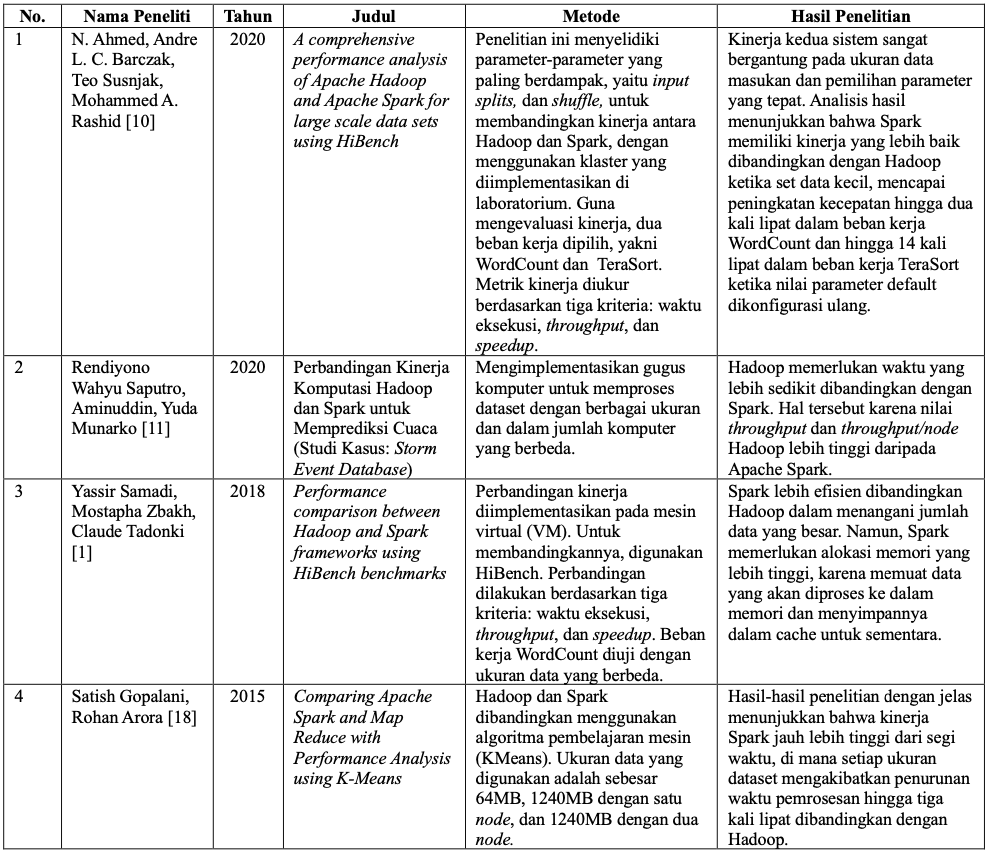
\includegraphics[width=1\textwidth]{figures/ch02/comparison-thesis}
%  \label{table:penelitian-dulu}
%\end{table}

\section{Konsep \textit{Big Data}}
\textit{Big Data} biasanya sering didefinisikan bersama dengan kompleksitas suatu data \cite{barosenAnalysisComparisonInterfacing2018}. Berbeda dengan tradisional data, \textit{Big Data} merujuk pada pertumbuhan data dalam berbagai format, baik dari struktur, semi-terstruktur, dan tidak terstruktur \cite{oussousBigDataTechnologies2018}. \textit{Big Data} memiliki banyak jenis sehingga membutuhkan teknologi yang lebih bertenaga serta algoritma yang lebih canggih. Pendekatan teknologi yang sering digunakan oleh \textit{Business Intelligence} biasanya tidak dapat lagi efisien jika digunakan.

\textit{Big Data} biasanya didefinisikan menjadi tiga karakteristik (3V), yaitu \textit{Volume, Velocity}, dan \textit{Variety} \cite{furhtIntroductionBigData2016}. \textit{Volume} berkaitan dengan jumlah data yang terbentuk atau dibuat secara terus menerus oleh beragam  perangkat, seperti telepon genggam dan aplikasi (sosial media, sensor, IoT). Jumlah data diharapkan tumbuh 5x lipat pada tahun 2020 \cite{furhtIntroductionBigData2016}. Selanjutnya, \textit{Velocity} memberikan makna bahwa data bertumbuh secara cepat dan harus diproses secara cepat juga untuk memberikan informasi yang berguna \cite{sandhuBigDataCloud2022}. YouTube adalah ilustrasi yang tepat untuk menggambarkan bagaimana pertumbuhan data begitu cepat. Terakhir, \textit{Variety} berkaitan dengan variasi sumber dan format data. 

Penerapan dari \textit{big data} tidak hanya terbatas pada pengumpulan dan penyimpanan data, tetapi juga meliputi analisis dan pengolahan data tersebut untuk menghasilkan wawasan yang berguna. Beberapa sektor yang telah menerapkan \textit{big data} secara luas meliputi kesehatan, keuangan, ritel, dan pemerintahan \cite{oussousBigDataTechnologies2018}. Dalam sektor kesehatan, \textit{big data} digunakan untuk menganalisis informasi pasien secara massal guna meningkatkan kualitas perawatan dan menemukan pola-pola penyakit. Sementara itu, di sektor keuangan, big data membantu dalam analisis risiko, deteksi penipuan, dan personalisasi layanan untuk pelanggan.

\section{Statistika Deskriptif}
Statistika deskriptif merupakan cabang statistika yang fokus pada pengorganisasian, penyajian, dan pengikhtisaran data \cite{rossIntroductoryStatistics2017}. Informasi yang diperoleh dari statistika deskriptif berguna untuk mendapatkan gambaran umum mengenai data dan untuk memahaminya secara lebih mendalam. Beberapa ukuran statistika deskriptif yang umum digunakan antara lain,

\begin{enumerate}
\item Maksimum (Max)

Maksimum (Max) merupakan nilai tertinggi dalam suatu kumpulan data. 

\begin{equation}
\text{Max} = \text{Nilai tertinggi dalam data}
\end{equation}

\item Minimum (Min)

Minimum (Min) merupakan nilai terendah dalam suatu kumpulan data. 

\begin{equation}
\text{Min} = \text{Nilai terendah dalam data}
\end{equation}

\item Rata-rata (Mean)

Rata-rata (Mean) merupakan nilai tengah dari suatu kumpulan data. Didefinisikan sebagai jumlah semua nilai data dibagi dengan jumlah total data.

\begin{equation}
\text{Mean} = \bar{x} = \frac{\sum_{i=1}^{n} x_i}{n}
\end{equation}

Keterangan:
\begin{itemize}
\item $\bar{x}$ adalah mean
\item $x_i$ adalah nilai data ke-i
\item $n$ adalah jumlah total data
\end{itemize}

\item Standar Deviasi (Std)

Standar deviasi (Std) merupakan ukuran penyebaran data terhadap mean. Semakin besar standar deviasi, semakin tersebar data dari mean. 

\begin{equation}
\text{Std} = s = \sqrt{\frac{\sum_{i=1}^{n} (x_i - \bar{x})^2}{n}}
\end{equation}

Keterangan:
\begin{itemize}
\item $s$ adalah standar deviasi
\item $x_i$ adalah nilai data ke-i
\item $\bar{x}$ adalah mean
\item $n$ adalah jumlah total data
\end{itemize}

\end{enumerate}

\section{Ekstraksi Fitur Teks (\textit{Text Feature Extraction})}
\textit{Ekstraksi Fitur Teks} adalah salah satu proses pada pembelajaran mesin (\textit{machine learning)} dan data analisis yang melibatkan identifikasi dan ekstraksi fitur yang relevan dari data mentah \cite{vijayakumarFusionBasedFeature2021}. Fitur-fitur tersebut nantinya akan digunakan untuk membuat data yang lebih informatif, sehingga dapat digunakan untuk klasifikasi, prediksi, dan klasterisasi. Ekstraksi fitur bertujuan untuk mengurangi kompleksitas data (atau yang sering disebut juga \textit{Data Dimensionality}) namun tetap menyimpan sebanyak mungkin informasi yang paling relevan. Hal ini bertujuan untuk meningkatkan performa dan efisiensi algoritma pada pembelajaran mesin dan mempermudah dalam proses analisis. Ekstraksi fitur dapat melibatkan membuat fitur baru (\textit{Feature Engineering}) atau memanipulasi data yang menghasilkan fitur yang berguna.
Ekstraksi fitur juga memainkan peran penting dalam banyak penerapan di dunia nyata, misalnya untuk pemrosesan teks dan \textit{Natural Language Processing} (NLP). Dalam skenario ini, data mentah mungkin mengandung banyak fitur yang tidak relevan atau berlebihan. Hal ini menyulitkan algoritma untuk memproses data secara akurat. Dengan melakukan ekstraksi fitur, fitur yang relevan dipisahkan dari fitur yang tidak relevan \cite{shakerFeatureExtractionBased2022}. Dengan lebih sedikit fitur yang harus diproses, kumpulan data menjadi lebih sederhana dan akurasi serta efisiensi analisis meningkat.

\subsection{\textit{Bag of Words} (BoW)}
BoW adalah teknik sederhana yang mengabaikan urutan dan struktur gramatikal kalimat, dan hanya berfokus pada frekuensi kemunculan kata dalam dokumen. Prosesnya melibatkan langkah-langkah berikut:

\begin{enumerate}
    \item \textbf{Tokenisasi:} Teks dipecah menjadi kata-kata individual (token).
    \item \textbf{Pembuatan Kosakata:} Daftar unik dari semua token yang ada dalam seluruh kumpulan dokumen dibuat. Ini disebut "kosakata".
    \item \textbf{Penghitungan Kata (Word Count): } Untuk setiap dokumen, frekuensi kemunculan setiap kata dalam kosakata dihitung. 
    \item \textbf{Representasi Vektor:} Setiap dokumen diwakili sebagai vektor, di mana setiap elemen vektor mewakili frekuensi kata tertentu dalam kosakata.
\end{enumerate}

BoW mudah diimplementasikan dan efisien, namun kelemahannya adalah kehilangan informasi kontekstual dan semantik. Kata-kata dengan frekuensi tinggi, meskipun kurang informatif, dapat mendominasi representasi vektor.

\subsection{\textit{Term Frequency-Inverse Document Frequency} (TF-IDF)}

TF-IDF mengatasi beberapa kelemahan BoW dengan mempertimbangkan pentingnya kata dalam dokumen dan koleksi dokumen \cite{qaiserTextMiningUse2018}. TF-IDF terdiri dari dua komponen:

\begin{enumerate}
    \item \textbf{\textit{Term Frequency} (TF): } Mengukur seberapa sering suatu kata muncul dalam dokumen.
    \item \textbf{\textit{Inverse Document Frequency} (IDF): } Mengukur seberapa penting suatu kata dalam seluruh koleksi dokumen. Kata-kata yang muncul di banyak dokumen (seperti kata "yang") memiliki IDF rendah, sementara kata-kata yang jarang muncul (dan kemungkinan lebih informatif) memiliki IDF tinggi.
\end{enumerate}

Dengan mengalikan TF dan IDF, kita mendapatkan nilai TF-IDF yang mencerminkan pentingnya kata dalam dokumen dan koleksi dokumen. Rumus umum untuk TF-IDF sebagai berikut, 

\begin{equation}
w_{ij} = tf_{ij} \times \log \left(\frac{N}{df_i}\right)
\end{equation}

Keterangan:

\begin{itemize}
    \item $w_{ij}$ adalah bobot tf-idf untuk kata $i$ dalam dokumen $j$;
    \item $tf_{ij}$ adalah frekuensi kemunculan kata $i$ dalam dokumen $j$ dibagi dengan total jumlah kata dalam dokumen $j$;
    \item $N$ adalah total jumlah dokumen dalam korpus;
    \item $df_i$ adalah jumlah dokumen dalam korpus yang mengandung kata $i$.
\end{itemize}

Sebagai contoh, misalkan kita ingin menghitung bobot TF-IDF untuk kata “\textit{British}” yang muncul 5 kali dalam sebuah dokumen yang berisi 100 kata. Dengan korpus yang berisi 4 dokumen, dimana 2 dokumen menyebutkan kata “British”, TF-IDF dapat dihitung sebagai berikut:

\begin{equation}
w_{British} = \frac{5}{100} \times \log \left(\frac{4}{2}\right) = 0.015
\end{equation}

TF-IDF meningkat seiring dengan peningkatan frekuensi kemunculan kata dalam dokumen, tetapi menurun seiring dengan peningkatan jumlah dokumen lain dalam korpus yang juga mengandung kata tersebut. Variasi dari skema pembobotan TF-IDF sering digunakan oleh mesin pencari sebagai alat utama dalam menilai dan meranking relevansi dokumen terhadap query pengguna.

\subsection{Penggunaan \textit{Word Count} dan \textit{Sort} pada BoW dan TF-IDF}

\begin{enumerate}
    \item \textbf{\textit{Word Count:}} Digunakan dalam kedua metode (BoW dan TF-IDF) untuk menghitung frekuensi kemunculan kata dalam dokumen.
    \item \textbf{\textit{Sort:}} Biasanya tidak digunakan secara langsung dalam proses BoW atau TF-IDF. Namun, pengurutan dapat digunakan untuk:
    \begin{itemize}
        \item \textbf{Memilih fitur:} Memilih fitur dengan nilai TF-IDF tertinggi untuk mengurangi dimensi data dan fokus pada kata-kata yang paling informatif. 
        \item \textbf{Visualisasi:} Mengurutkan kata berdasarkan frekuensi atau nilai TF-IDF dapat membantu dalam visualisasi dan analisis data.
    \end{itemize}
\end{enumerate}

\section{Komputasi Awan \textit{(Cloud Computing)}}
Komputasi awan didefinisikan sebagai sistem informasi yang memungkinkan akses mudah ke sumber daya komputasi atau layanan komputasi sesuai permintaan (\textit{on demand}), misalnya segala sesuatu mulai dari aplikasi (Google Mail, Microsft One Drive, Siakad Itera) hingga pusat data di seluruh internet dengan sistem bayar sesuai penggunaan.
Sistem komputasi awan saat ini menyediakan tiga layanan utama:
\begin{enumerate}
	\item \textit{Infrastructure as a service} (IaaS), adalah layanan awan yang menawarkan kepada pengguna untuk mengatur dan mengonfigurasikan sumber daya yang dibutuhkan untuk menjalankan aplikasi dan sistem IT. Jenis IaaS biasanya berbentuk komputasi, penyimpanan, dan sumber daya jaringan yang dibuat sebagai layanan.
	\item \textit{Platform as a service} (PaaS), adalah layanan awan yang memungkinkan pengguna untuk mengembangkan, mengelola, dan menjalankan aplikasi di lingkungan yang dikontrol oleh penyedia layanan, tanpa harus khawatir dengan infrastruktur yang mendasarinya. 
	\item \textit{Software as a service} (SaaS), adalah layanan awan yang mengacu pada aplikasi yang berjalan pada infrastruktur awan yang di-\textit{hosting} oleh vendor atau penyedia layanan dan tersedia untuk pengguna akhir melalui browser web. 
\end{enumerate}
Komputasi awan menjadi salah satu aspek terpenting dalam menjalankan komputasi yang kompleks, misalnya untuk menjalankan Hadoop atau Spark. Salah satu komputasi awan yang dapat diandalkan adalah DigitalOcean. DigitalOcean dibentuk pada tahun 2012 untuk memenuhi kebutuhan pengembang untuk mendapatkan akses komputasi awan yang mudah dimengerti dan terjangkau \cite{DigitalOcean}. Salah satu produk DigitalOcean yang sering digunakan adalah Droplet, \textit{easy-to-use} komputer virtual yang siap digunakan dalam hitungan menit. Pengguna dapat memilih lokasi dimana komputer akan dijalankan, bagaimana konfigurasi prosesor serta memori, memilih sistem operasi apa yang akan digunakan, dan banyak hal lainnya.

\section{\textit{Shell Script}}
\textit{Shell script} merupakan serangkaian perintah yang dieksekusi dalam lingkungan sistem operasi Unix atau Unix-like \cite{newhamLearningBashShell2005}. \textit{Shell script} memungkinkan pengguna untuk mengotomatiskan tugas-tugas rutin, melakukan pemrosesan file, dan bahkan membangun aplikasi yang kompleks dengan menggunakan perintah-perintah shell. \textit{Shell script} umumnya ditulis menggunakan bahasa pemrograman shell, seperti Bash (Bourne Again Shell), yang merupakan shell standar pada sebagian besar sistem operasi Linux dan MacOS.
Sebagai contoh, dalam mengelola pencadangan sistem, seorang administrator dapat membuat \textit{shell script} sederhana yang menjalankan perintah-perintah untuk menyalin file-file penting ke lokasi penyimpanan cadangan secara berkala. Skrip ini dapat dijadwalkan untuk berjalan secara otomatis menggunakan \textit{cron job}, sehingga proses pencadangan dapat dilakukan tanpa campur tangan manusia secara berkala. Dengan menggunakan variabel dan logika sederhana, administrator dapat dengan mudah menyesuaikan skrip ini untuk memenuhi kebutuhan pencadangan spesifik sistem mereka. Dengan demikian, \textit{shell script} tidak hanya menghemat waktu dan tenaga, tetapi juga meningkatkan kehandalan dan konsistensi dalam administrasi sistem.

\begin{figure}[h]
    \centering
    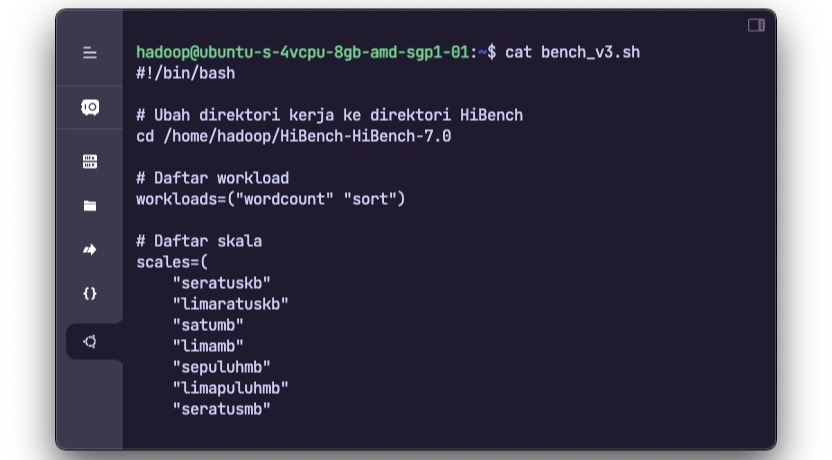
\includegraphics[width=0.75\textwidth]{figures/ch02/contoh-bash}
    \caption{Contoh Shell Script yang Digunakan pada Penelitian}
    \label{fig:contoh-bash}
\end{figure}

Gambar \ref{fig:contoh-bash} menampilkan sebuah contoh potongan \textit{shell script} yang digunakan dalam penelitian ini. Berikut adalah penjelasan lebih rinci mengenai skrip tersebut,
\begin{enumerate}
    \item \textbf{Baris 1:} Mendefinisikan interpreter Bash untuk menjalankan skrip.
    \item \textbf{Baris 3-4: } Mengubah direktori kerja ke direktori HiBench.
    \item \textbf{Baris 6-7: } Mendefinisikan daftar \textit{(list)} \textit{workLoads} berisi macam-macam beban kerja, yaitu \textit{wordcount} dan \textit{sort}.
    \item \textbf{Baris 9-15: } Mendefinisikan daftar \textit{scales} berisi skala input data.
\end{enumerate}

\section{\textit{CPU Bound} dan \textit{I/O Bound}}

Terdapat dua jenis beban kerja pada pemrosesan data berdasarkan karakteristik dan kebutuhan sumber daya yang berbeda, yaitu \textit{CPU-bound} dan \textit{I/O-bound}. Proses \textit{CPU-bound} (Gambar \ref{fig:cpu-bound} atas) sangat bergantung pada kemampuan pemrosesan data oleh \textit{Central Processing Unit} (CPU). Proses ini menghabiskan sebagian besar waktunya dalam menjalankan instruksi CPU dan jarang berinteraksi dengan sistem I/O (Input/Output). Sebaliknya, proses \textit{I/O-bound} (Gambar \ref{fig:cpu-bound} bawah) lebih banyak menghabiskan waktu dalam menunggu operasi I/O, seperti akses disk, jaringan, atau komunikasi peripheral. CPU dalam proses ini mungkin hanya digunakan sesaat untuk memproses data yang baru saja diperoleh dari I/O. 

Proses \textit{CPU-bound} memiliki interval waktu yang panjang untuk menjalankan instruksi CPU, dan jarang melakukan operasi I/O, yang dikenal sebagai \textit{CPU bursts} yang panjang dan jarang. Sementara itu, proses \textit{I/O-bound} memiliki interval waktu yang pendek untuk menjalankan instruksi CPU, dan sering melakukan operasi I/O, sehingga memiliki \textit{CPU bursts} yang pendek dan sering. 

\begin{figure}[h!]
    \centering
    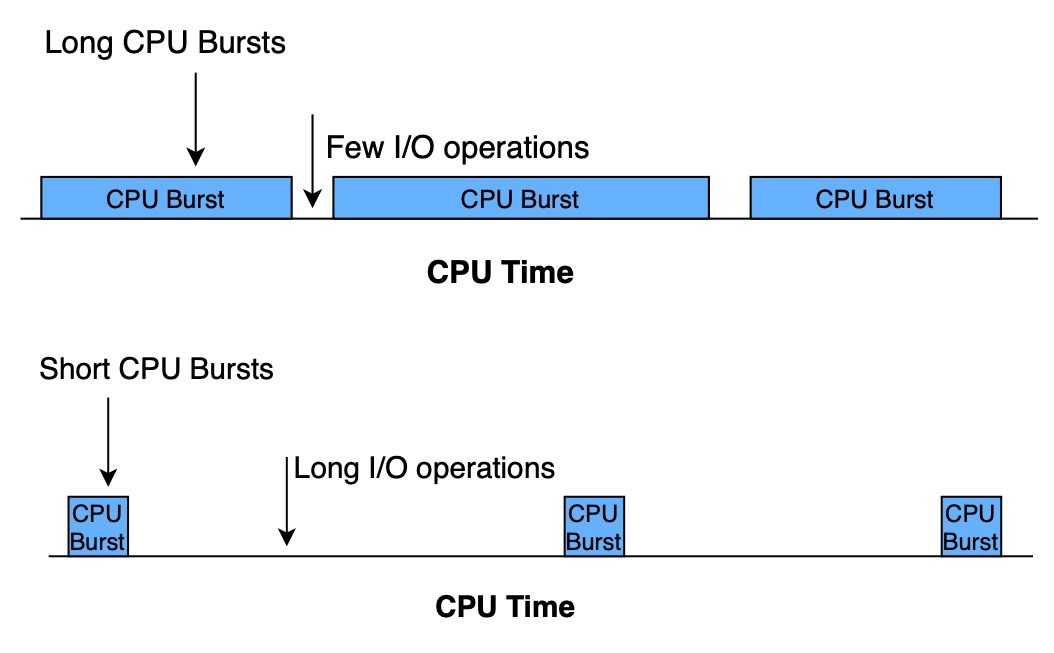
\includegraphics[width=0.8\textwidth]{figures/ch02/cpu-io-bound.jpg}
    \caption{\textit{CPU-I/O Bound} \cite{baeldungGuideCpuBoundBound2021}}
    \label{fig:cpu-bound}
\end{figure}


\section{MapReduce}
MapReduce adalah model pemrograman dan implementasi teknik pemrosesan data berukuran besar yang pertama kali dipopulerkan oleh Google pada tahun 2004\cite{kaliaAnalysisHadoopMapReduce2021}. MapReduce menawarkan pemrosesan data yang dapat diandalkan serta \textit{fault-tolerant manner} (tahan terhadap kesalahan).  MapReduce berjalan secara paralel dan berada pada lingkungan komputasi terdistribusi \cite{cTaskFailureResilience2020}. Model ini mengadopsi arsitektur tersentraliasi, yaitu satu \textit{node} berperan sebagai \textit{master} dan \textit{node} yang lain berperan sebagai \textit{workers} atau \textit{slave} \cite{herodotouHadoopPerformanceModels2011, bakratsasHadoopMapReducePerformance2018}. \textit{Master node} bertanggung jawab untuk melakukan penjadwalan kerja, dan \textit{slave node} berperan untuk menjalankan eksekusi kerja. 

\begin{figure}[h!]
    \centering
    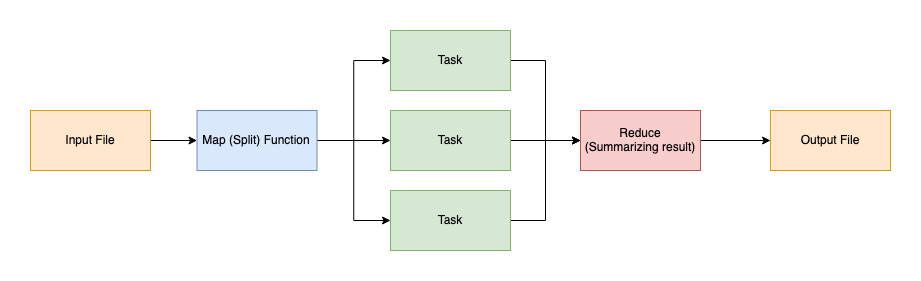
\includegraphics[width=1\textwidth]{figures/ch02/mapreduce-scheme.png}
    \caption{Cara Kerja MapReduce}
    \label{fig:mapreduce-flow}
\end{figure}

MapReduce terdiri dari fungsi \textit{Map} dan fungsi \textit{Reduce} \cite{gandomiHybSMRPHybridScheduling2019}. Kedua fungsi ini tersebar di seluruh \textit{slave node} yang terhubung dalam klaster dan berjalan secara paralel. Fungsi \textit{Map} berperan untuk membagi masalah besar menjadi masalah yang lebih kecil dan mendistribusikannya ke \textit{slave node}. Hasil pemrosesan dari \textit{slave node} akan dikumpulkan oleh \textit{master node} melalui fungsi \textit{Reduce}. Sesuai dengan Gambar \ref{fig:mapreduce-flow}, hasil dari proses \textit{Reduce} yang akan dikirimkan sebagai hasil akhir proses MapReduce.  

\subsection{Apache Hadoop}
Apache Hadoop adalah perangkat lunak sumber terbuka yang ditulis dengan bahasa pemrograman Java untuk pemrosesan dan penyimpanan data menggunakan komputasi terdistribusi \cite{ApacheHadoop}. Hadoop dapat diinstalasi pada satu \textit{node} komputer, atau ratusan \textit{node} komputer yang digabungkan dalam sebuah klaster \cite{maneasEvolutionHadoopDistributed2018}. Berkaitan dengan pemrosesan data, Hadoop mengimplementasikan model MapReduce untuk pemrosesan data secara paralel dan cepat. Selain itu, Hadoop menyediakan sistem penyimpanan data terdistribusi yang dikenal sebagai Hadoop Distributed File System (HDFS) untuk akses data, pemrosesan, dan komputasi \cite{dabasAnalysisCommentsYoutube2019}. Arsitektur Hadoop secara umum dapat dilihat pada Gambar \ref{fig:hadoop-str}.

\begin{figure}[h!]
    \centering
    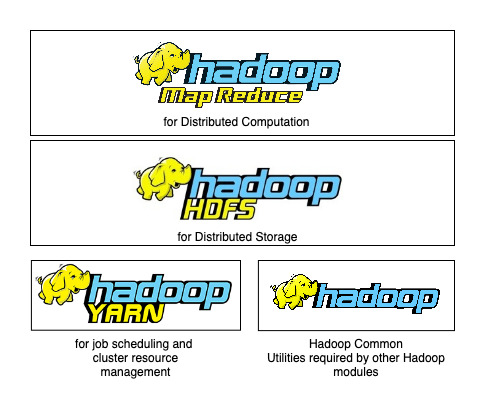
\includegraphics[width=0.6\textwidth]{figures/ch02/hadoop-str}
    \caption{Arsitektur Hadoop}
    \label{fig:hadoop-str}
\end{figure}

\subsection{Mode Kerja Hadoop}
Hadoop dapat dijalankan dalam tiga mode operasi yang berbeda yaitu \textit{standalone, pseudo-distributed}, dan \textit{fully distributed} \cite{johnDataLakeEnterprises2017}. Dalam \textit{standalone mode}, semua proses Hadoop berjalan pada satu node tunggal menggunakan sistem berkas lokal tanpa memerlukan konfigurasi kustom pada Hadoop seperti pada Gambar \ref{fig:hadoop-modes}. 

\begin{figure}[h!]
    \centering
    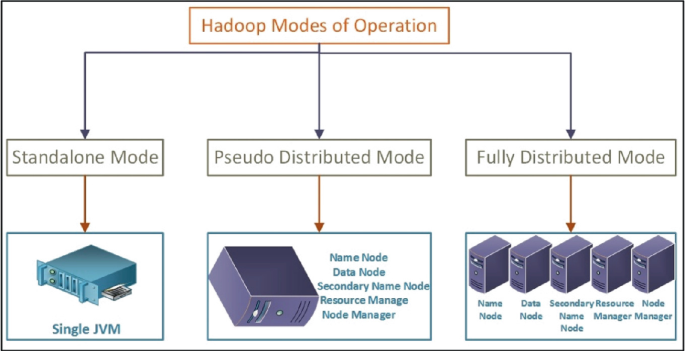
\includegraphics[width=0.9\textwidth]{figures/ch02/hadoop-modes}
    \caption{Mode Kerja Hadoop \cite{khataiImplementationTextMining2021}}
    \label{fig:hadoop-modes}
\end{figure}

\textit{Pseudo-distributed mode} menjalankan semua komponen Hadoop pada satu node tunggal tetapi menyimulasikan kluster dengan komunikasi antar proses melalui socket jaringan, sehingga memerlukan konfigurasi pada berkas \textit{core-site, mapred-site}, dan \textit{hdfs-site}. Sedangkan \textit{fully distributed mode} menyebarkan proses Hadoop ke beberapa node dalam kluster sebenarnya yang biasanya digunakan untuk tahap produksi. \textit{Fully distributed mode} mendukung skalabilitas, ketersediaan tinggi, dan keamanan dengan memerlukan instalasi Hadoop dan konfigurasi kluster pada setiap node.

\subsection{Hadoop Distributed File System (HDFS)}
\textit{Hadoop Distributed File System} adalah sistem file terdistribusi yang dikembangkan sebagai bagian dari Hadoop \cite{abhishekIntegratedHadoopCloud2017}. HDFS dirancang khusus untuk menyimpan data dalam jumlah besar dan memungkinkan pemrosesan data secara paralel. Beberapa fitur utama dari HDFS antara lain skalabilitas, toleransi kesalahan, \textit{streaming access}, dan cocok untuk aplikasi \textit{batch} seperti MapReduce.

\begin{figure}[h!]
    \centering
    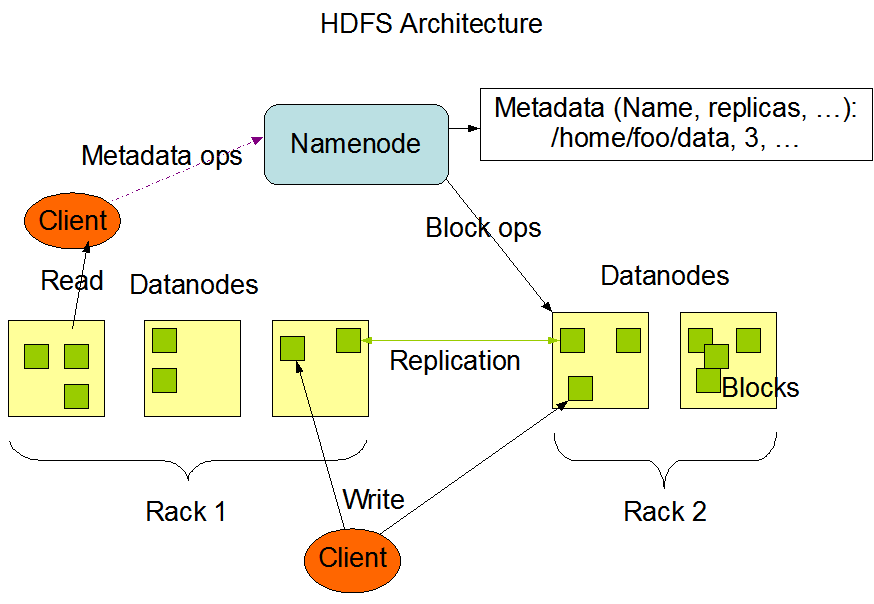
\includegraphics[width=0.8\textwidth]{figures/ch02/hdfsarchitecture}
    \caption{Arsitektur HDFS \cite{ApacheHadoopHDFS}}
    \label{fig:hdfs-arch}
\end{figure}

Secara struktur, HDFS terdiri dari NameNode sebagai \textit{node master} yang mengelola \textit{metadata} dan \textit{namespace}, serta DataNode sebagai \textit{node slave} yang bertugas menyimpan data sebenarnya dalam bentuk blok seperti pada Gambar \ref{fig:hdfs-arch}. Berkas di HDFS dipartisi menjadi satu atau lebih blok berukuran 64MB atau 128MB, kemudian didistribusikan dan disimpan di beberapa DataNode. Setiap blok direplikasi (biasanya 3x) di DataNode yang berbeda untuk toleransi kesalahan. Replikasi blok di \textit{node/rack} yang berbeda juga meningkatkan ketersediaan HDFS.

Dengan desain terdistribusi, HDFS sangat populer digunakan bersama framework Hadoop untuk memproses \textit{big data} \cite{almansouriHadoopDistributedFile2019}. Namun, ketergantungan pada \textit{single} NameNode dan performa akses data acak yang kurang optimal menjadi kelemahan utama HDFS. Secara keseluruhan, HDFS telah terbukti menjadi pilihan matang untuk penyimpanan data massal secara terdistribusi.

\subsection{Hadoop YARN}
\textit{Hadoop YARN} (\textit{Yet Another Resource Negotiator}) adalah manajer sumber daya dan sistem penjadwalan untuk kluster Hadoop. Komponen ini diperkenalkan dalam Hadoop 2.x sebagai evolusi dari Hadoop MapReduce 1.x, yang mengintegrasikan manajemen sumber daya dan pemrosesan data dalam satu sistem. YARN memungkinkan kluster untuk menjalankan berbagai aplikasi secara bersamaan dengan efisiensi yang lebih baik.  YARN memisahkan fungsi manajemen sumber daya dari mekanisme pemrosesan data, yang sebelumnya keduanya tertanam dalam MapReduce. Dengan demikian, YARN dapat mendukung berbagai paradigma pemrosesan data di atas Hadoop, selain MapReduce, seperti \textit{real-time processing} dan \textit{graph processing}.

\begin{figure}[h!]
    \centering
    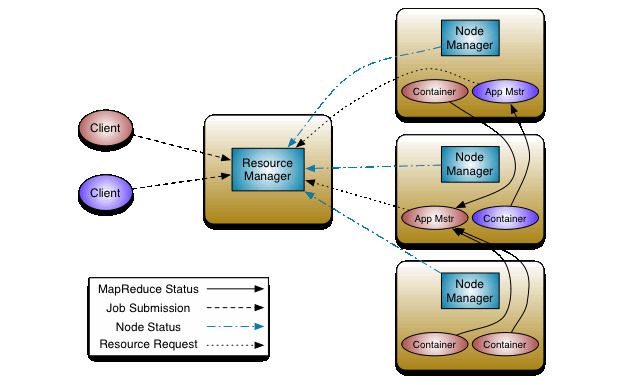
\includegraphics[width=0.8\textwidth]{figures/ch02/yarn-arch}
    \caption{Arsitektur YARN \cite{ApacheHadoopApache}}
    \label{fig:yarn_arch}
\end{figure}

Struktur utama YARN terdiri dari ResourceManager yang bertugas mengkoordinasikan alokasi sumber daya di seluruh kluster, dan NodeManager yang berjalan di setiap \textit{node} untuk mengawasi penggunaan sumber daya dan mengelola \textit{container} tempat aplikasi dijalankan. \textit{ApplicationMaster} adalah komponen khusus untuk setiap aplikasi yang bertanggung jawab untuk negosiasi sumber daya dengan ResourceManager dan bekerja dengan NodeManager untuk menjalankan dan memantau \textit{tasks} seperti pada Gambar \ref{fig:yarn_arch}.

\section{Apache Spark}
Apache Spark diperkenalkan oleh Apache Software Foundation sebagai \textit{framework} pemrosesan data paralel \textit{open-source} yang dirancang untuk mempercepat pemrosesan \textit{big data} dibandingkan dengan  Hadoop MapReduce \cite{ApacheSparkUnified}. Meskipun sama-sama menggunakan model pemrosesan MapReduce, Spark bukanlah hasil modifikasi dari Hadoop MapReduce\cite{KOMPARASIKECEPATANHADOOP}. Hal ini dikarenakan Spark menggunakan teknologi tersendiri yaitu \textit{Resilient Distributed Datasets} (RDDs) yang memungkinkan Spark memproses data secara \textit{in-memory} sehingga lebih cepat. Selain itu, Spark memiliki klaster pengolahan data tersendiri sehingga dapat berjalan independen tanpa Hadoop. Dengan performa tinggi serta dukungan untuk pemrosesan data secara interaktif, Spark banyak digunakan untuk pemrosesan data skala besar. Komponen yang terdapat pada Spark dapat dilihat pada Gambar \ref{fig:spark-component}

\begin{figure}[h]
    \centering
    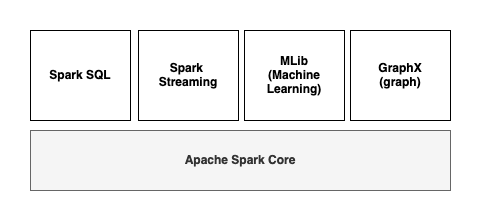
\includegraphics[width=0.6\textwidth]{figures/ch02/spark-contain}
    \caption{Komponen Spark}
    \label{fig:spark-component}
\end{figure}

\subsection{Arsitektur Spark}

Arsitektur Spark dirancang untuk pemrosesan data terdistribusi yang efisien dan cepat seperti pada Gambar \ref{fig:spark-arch}. Komponen utamanya meliputi \textit{Spark Driver, Cluster Manager}, dan \textit{Spark Executor}. \textit{Spark Driver} berperan sebagai otak operasi, bertanggung jawab untuk mengonversi program pengguna menjadi tugas-tugas, menjadwalkan tugas pada \textit{executor}, dan mengelola keseluruhan alur kerja. \textit{Cluster Manager}, yang dapat berupa YARN, Mesos, atau mode \textit{standalone} Spark, menangani alokasi sumber daya dan peluncuran \textit{executor} pada \textit{node-node cluster}. \textit{Spark Executor}, yang berjalan pada \textit{node-node cluster}, menjalankan tugas-tugas pemrosesan data yang diberikan oleh \textit{driver} dan menyediakan penyimpanan dalam memori untuk data yang di-\textit{cache}. Interaksi antara komponen-komponen ini memungkinkan pemrosesan data paralel yang cepat dan toleransi kesalahan yang tinggi. Arsitektur Spark yang fleksibel mendukung berbagai bahasa pemrograman dan sistem penyimpanan data, menjadikannya solusi ideal untuk berbagai kasus penggunaan data besar.

\begin{figure}[h]
    \centering
    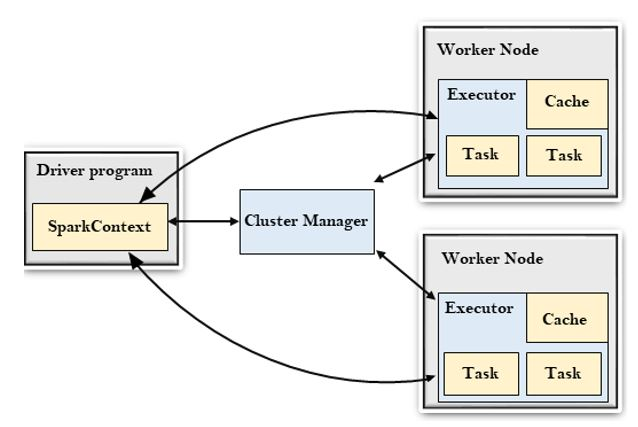
\includegraphics[width=0.6\textwidth]{figures/ch02/spark-arch.jpeg}
    \caption{Arsitektur Spark}
    \label{fig:spark-arch}
\end{figure}

\subsection{Integrasi Hadoop dan Spark}
Integrasi Spark dengan Hadoop dapat dilakukan melalui tiga metode berbeda seperti pada Gambar \ref{fig:spark-x-hadoop}  \cite{ApacheSparkIntroduction}. Pertama, metode \textit{Standalone} mengharuskan Spark menempati tempat di atas HDFS (\textit{Hadoop Distributed File System}). Dalam skenario ini, Spark dan MapReduce berjalan berdampingan untuk menangani semua pekerjaan Spark pada kluster. Kedua, metode Hadoop Yarn memungkinkan Spark berjalan pada Yarn tanpa memerlukan instalasi sebelumnya atau akses \textit{root}. Hal ini memfasilitasi integrasi Spark ke dalam ekosistem Hadoop, atau memungkinkan komponen lain berjalan di atas integrasi Hadoop dan Spark. Terakhir, metode \textit{Spark in MapReduce} (SIMR). Dengan SIMR, pengguna dapat memulai Spark dan menggunakan \textit{shell}-nya tanpa memerlukan akses administratif. 

\begin{figure}[h!]
    \centering
    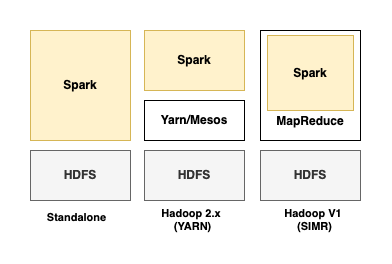
\includegraphics[width=0.7\textwidth]{figures/ch02/sparkxhadoop}
    \caption{Integrasi Spark dan Hadoop}
    \label{fig:spark-x-hadoop}
\end{figure}

%\section{\textit{Data Sharing} pada MapReduce dan Spark}
\subsection{Keterbatasan \textit{Data Sharing} pada MapReduce}

MapReduce, sebagai kerangka kerja pemrosesan data terdistribusi, mengandalkan sistem penyimpanan eksternal yang stabil, seperti HDFS, untuk berbagi data antar tugas (\textit{job}). Hal ini mengakibatkan inefisiensi karena beberapa alasan, yaitu:

\begin{enumerate}
    \item \textbf{Replikasi Data:} Data perlu direplikasi ke beberapa node untuk toleransi kesalahan dan paralelisme. Replikasi ini memakan waktu dan bandwidth jaringan.
    \item \textbf{Serialisasi/Deserialisasi:} Data perlu diubah formatnya (serialisasi) sebelum dikirim melalui jaringan dan diubah kembali (deserialisasi) di simpul tujuan. Proses ini menambah beban komputasi.
    \item \textbf{\textit{Disk} I/O:} Akses data dari dan ke disk cenderung lambat dibandingkan dengan akses memori. Pada MapReduce, setiap operasi baca-tulis data melibatkan interaksi dengan \textit{disk}, yang memperlambat performa.
\end{enumerate}

Keterbatasan ini terlihat jelas pada aplikasi yang membutuhkan operasi iteratif, di mana hasil antara dari satu tugas perlu digunakan kembali oleh tugas berikutnya. Pada MapReduce, setiap iterasi memerlukan pembacaan dan penulisan data ke HDFS, seperti yang diilustrasikan pada Gambar \ref{fig:iterative_operations_on_mapreduce}. Akibatnya, aplikasi iteratif pada MapReduce cenderung lambat dan tidak efisien.

\begin{figure}[h]
    \centering
    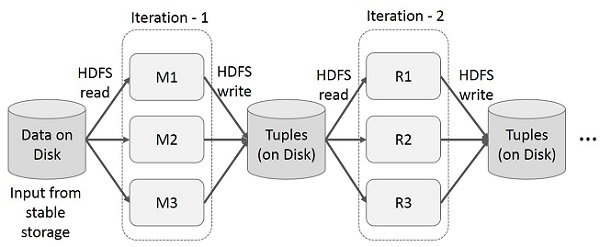
\includegraphics[width=1\textwidth]{figures/ch02/iterative_operations_on_mapreduce}
    \caption{\textit{Data Sharing} pada MapReduce \cite{ApacheSparkRDD}}
    \label{fig:iterative_operations_on_mapreduce}
\end{figure}

\subsection{Solusi \textit{Data Sharing} dengan Spark RDD}

Spark mengatasi keterbatasan MapReduce dengan memperkenalkan RDD, yaitu koleksi data terdistribusi yang disimpan dalam memori. RDD bersifat \textit{immutable}, artinya data tidak dapat diubah setelah dibuat, dan \textit{fault-tolerant}, artinya data dapat dipulihkan jika terjadi kegagalan node.

Dengan menyimpan data dalam memori, RDD memungkinkan akses data yang jauh lebih cepat dibandingkan dengan akses disk pada MapReduce. Selain itu, RDD mendukung \textit{lazy evaluation}, di mana operasi pada RDD tidak dieksekusi langsung, melainkan disimpan sebagai \textit{lineage} atau urutan operasi yang perlu dilakukan. Hal ini memungkinkan Spark untuk mengoptimalkan eksekusi tugas dan mengurangi overhead komputasi.

Pada aplikasi iteratif, RDD dapat menyimpan hasil antara dalam memori dan membagikannya antar tugas tanpa perlu mengakses disk, seperti yang ditunjukkan pada Gambar \ref{fig:iterative_operations_on_spark_rdd}. Dengan demikian, Spark RDD memungkinkan eksekusi aplikasi iteratif yang jauh lebih cepat dan efisien dibandingkan dengan MapReduce.

\begin{figure}[h]
    \centering
    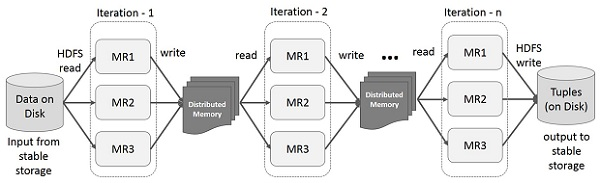
\includegraphics[width=1\textwidth]{figures/ch02/iterative_operations_on_spark_rdd}
    \caption{\textit{Data Sharing} pada RDD \cite{ApacheSparkRDD}}
    \label{fig:iterative_operations_on_spark_rdd}
\end{figure}

\section{HiBench}
HiBench memudahkan dalam eksekusi pengukuran berbagai beban kerja karena HiBench sudah membungkus sekumpulan perintah dalam bentuk \textit{shell script}\cite{samadiPerformanceComparisonHadoop2018}. Pengguna hanya perlu menjalankan perintah untuk HiBench melakukan persiapan data. Selanjutnya, pengguna bisa langsung melakukan pengukuran beban kerja. Hasilnya dapat terlihat langsung pada laporan HiBench. Secara umum, alur kerja HiBench terlihat seperti pada Gambar \ref{fig:hibench-process-flow}.

\begin{figure}[h]
    \centering
    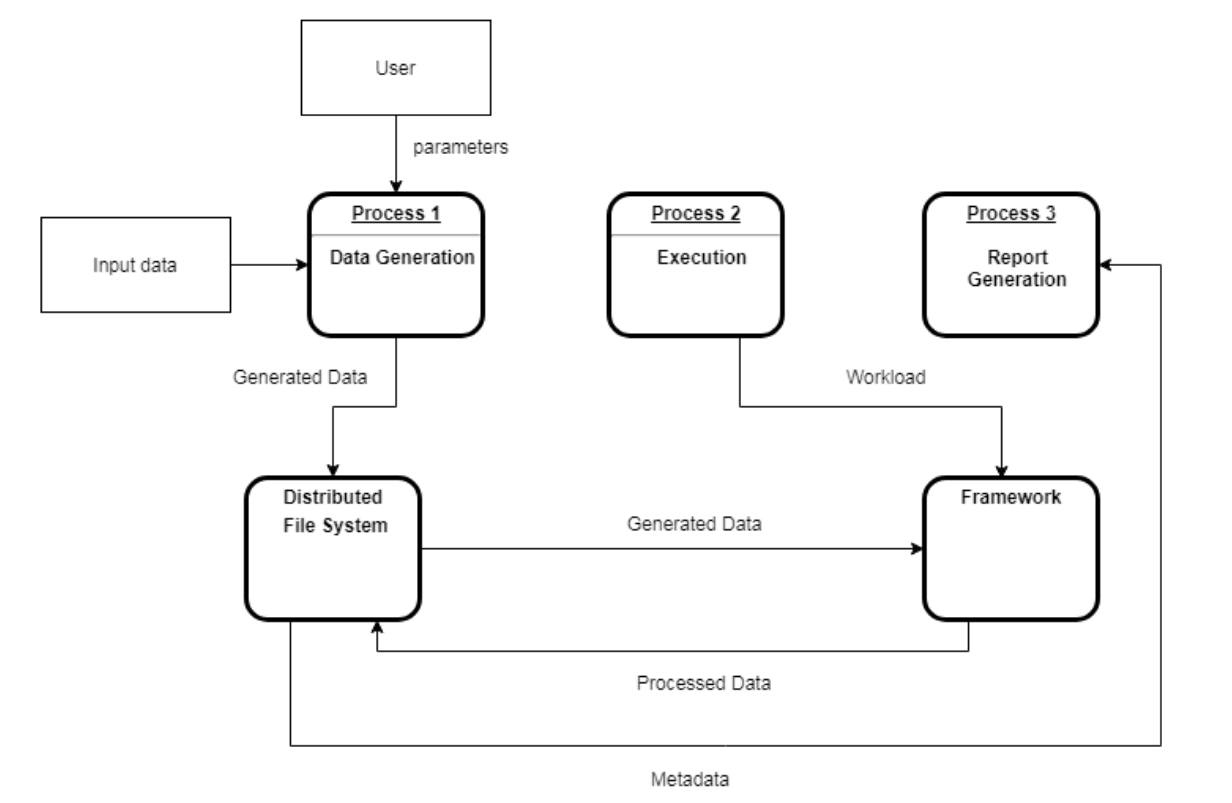
\includegraphics[width=1\textwidth]{figures/ch02/hibench-flow}
    \caption{Proses yang Terjadi di HiBench \cite{barosenAnalysisComparisonInterfacing2018}}
    \label{fig:hibench-process-flow}
\end{figure}

HiBench terdiri dari 3 proses utama. Proses pertama, pengguna melakukan konfigurasi parameter \textit{Data Generation}. Selanjutnya, \textit{Data Generation} akan melakukan pembentukan data yang nantinya akan disimpan pada \textit{Distributed File System} (DFS). Data ini yang akan digunakan pada proses selanjutnya. Proses kedua adalah proses eksekusi. Pengguna akan memicu salah satu beban kerja pada HiBench. Selanjutnya, HiBench akan memberi perintah kepada perangkat lunak (Hadoop/Spark) untuk menjalankan beban kerja tersebut. Setiap melakukan pengukuran, data yang digunakan adalah data dari \textit{Distributed File System} yang sebelumnya sudah dibentuk. Hasil dari eksekusi ini akan disimpan kembali di DFS. Proses terakhir adalah proses pembentukan laporan. Hasil dari proses sebelumnya akan diambil serta akan dibuatkan laporan secara otomatis.
Dalam laporan otomatis yang diberikan oleh HiBench, terdapat beberapa metriks yang tersedia, meliputi \textit{Execution Time} dan \textit{Throughput}. \textit{Execution Time} memiliki makna seberapa lama suatu kejadian berlangsung. Waktu yang dihitung adalah waktu diantara waktu awal dan waktu terakhir kejadian. Metriks ini dihitung dalam skala detik. Selanjutnya, \textit{Throughput} menghitung berapa banyak unit informasi yang dapat diproses oleh sistem dalam waktu tertentu. Metriks ini dinyatakan dalam \textit{byte}/detik.


\subsection{Beban Kerja \textit{Micro Benchmark} dan Sumber Data}
HiBench versi 7.1 memiliki 29 beban kerja (\textit{workload}) yang dapat diuji \cite{IntelbigdataHiBench2023}. Beban kerja ini dikategorikan menjadi 7 kategori, yaitu \textit{micro, ml (machine learning), sql, graph, websearch and streaming}. Tabel \ref{table:workload-list-hibench} menunjukkan macam-macam beban kerja yang dapat diuji. \textit{Workload name} mengindikasikan algoritma utama atau operasi apa yang dilakukan. \textit{Workload type} merepresentasikan kategori dari beban kerja. \textit{Operation types} menunjukkan klasifikasi jenis operasi yang dilakukan. \textit{Workload Submission Policy} berguna untuk mengetahui bagaimana cara pengguna untuk mengatur atau mengonfigurasikan beban kerja.

\begin{table}[h]
  \centering
  \caption{Beban Kerja pada HiBench \cite{barosenAnalysisComparisonInterfacing2018}}
  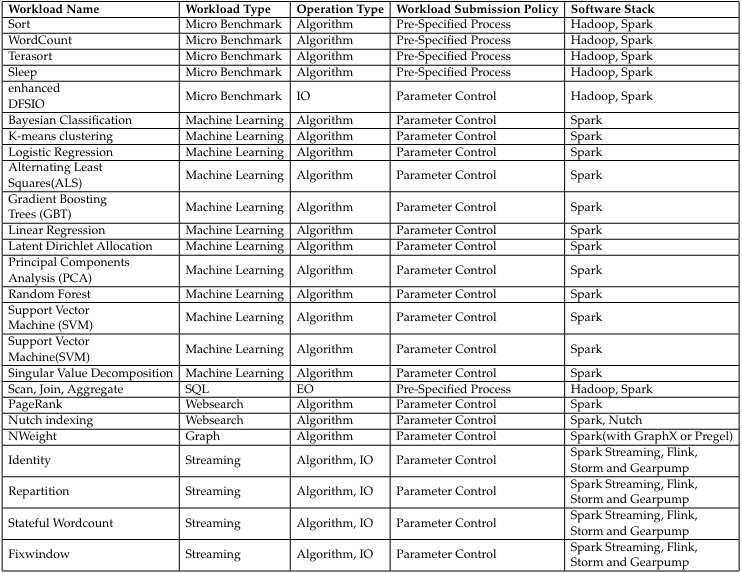
\includegraphics[width=1\textwidth]{figures/ch02/workload-hibench}
  \label{table:workload-list-hibench}
\end{table}

Beban kerja \textit{micro benchmarks} merupakan kategori khusus yang dirancang untuk menguji kemampuan \textit{raw processing power} \cite{barosenAnalysisComparisonInterfacing2018}. Dalam kategori ini, terdapat dua beban kerja populer, yaitu Sort, dan WordCount \cite{huangHiBenchBenchmarkSuitea}. Beban kerja Sort dan WordCount merepresentasikan pekerjaan MapReduce \cite{deanMapReduceSimplifiedData2004}. Beban kerja Sort akan mengurutkan setiap kata dalam berkas input. Beban kerja WordCount akan melakukan tugas pemetaan (\textit{map task}) dan mengeluarkan output (kata, 1) untuk setiap kata dalam inputnya.  Data masukan untuk beban kerja Sort dan WordCount dihasilkan menggunakan program RandomTextWriter yang nantinya akan dibuat melalui proses \textit{Data Generation}. 

\subsection{\textit{Data Generation} pada \textit{Word Count} dan \textit{Sort}}
\textit{Data generation} merupakan tahapan krusial dalam benchmark menggunakan HiBench, khususnya untuk beban kerja \textit{Word Count} dan \textit{Sort}. Tahapan ini bertanggung jawab untuk membentuk data acak yang akan diproses oleh kedua beban kerja tersebut. Tujuannya adalah untuk menyimulasikan skenario nyata dengan input data yang bervolume besar dan beragam.

Pada HiBench, skrip \textit{prepare.sh} seperti pada Algoritma \ref{algo:data-gen} berperan penting dalam menyiapkan data untuk beban kerja. Skrip ini mengeksekusi program \textit{randomtextwriter} yang terdapat dalam paket Hadoop. \textit{randomtextwriter} menghasilkan sekumpulan data acak yang terdiri dari kata-kata yang diambil dari daftar kata yang telah ditentukan. Jumlah data yang dihasilkan, jumlah \textit{map}, dan jumlah \textit{reduce} dapat dikonfigurasi melalui parameter-parameter yang diberikan kepada skrip \textit{prepare.sh}.

\begin{lstlisting}[language=bash, caption=Skrip yang Digunakan HiBench pada Tahap \textit{Data Generation}, label=algo:data-gen]
#!/bin/bash

current_dir=`dirname "$0"`
current_dir=`cd "$current_dir"; pwd`
root_dir=${current_dir}/../../../../../
workload_config=${root_dir}/conf/workloads/micro/sort.conf
. "${root_dir}/bin/functions/load_bench_config.sh"

enter_bench HadoopPrepareSort ${workload_config} ${current_dir}
show_bannar start

rmr_hdfs $INPUT_HDFS || true
START_TIME=`timestamp`

run_hadoop_job ${HADOOP_EXAMPLES_JAR} randomtextwriter \
    -D mapreduce.randomtextwriter.totalbytes=${DATASIZE} \
    -D mapreduce.randomtextwriter.bytespermap=$(( ${DATASIZE} / ${NUM_MAPS} )) \
    -D mapreduce.job.maps=${NUM_MAPS} \
    -D mapreduce.job.reduces=${NUM_REDS} \
    ${INPUT_HDFS}
END_TIME=`timestamp`
show_bannar finish
leave_bench
\end{lstlisting}

Dalam penerapannya, \textit{random text writer} akan menghitung jumlah total \textit{map task} yang diperlukan berdasarkan konfigurasi dan status kluster Hadoop. Setiap \textit{map task} akan menulis data hingga mencapai jumlah bita yang telah dikonfigurasi, menghasilkan kata acak sesuai dengan panjang yang telah ditentukan. Kata acak tersebut berasal dari kamus (\textit{dictionary}) yang sebelumnya sudah didefinisikan seperti pada Gambar \ref{fig:contoh-data}.

Jika diberikan input yang pasti, misalnya 100 KB, \textit{random text writer} memungkinkan menghasilkan output dengan ukuran tersebut tanpa pemotongan kata, karena \textit{mapper} menghasilkan kata acak dalam satuan kata lengkap dan menghitung panjang kata-kata tersebut sebelum menulisnya.

\begin{figure}[h]
    \centering
    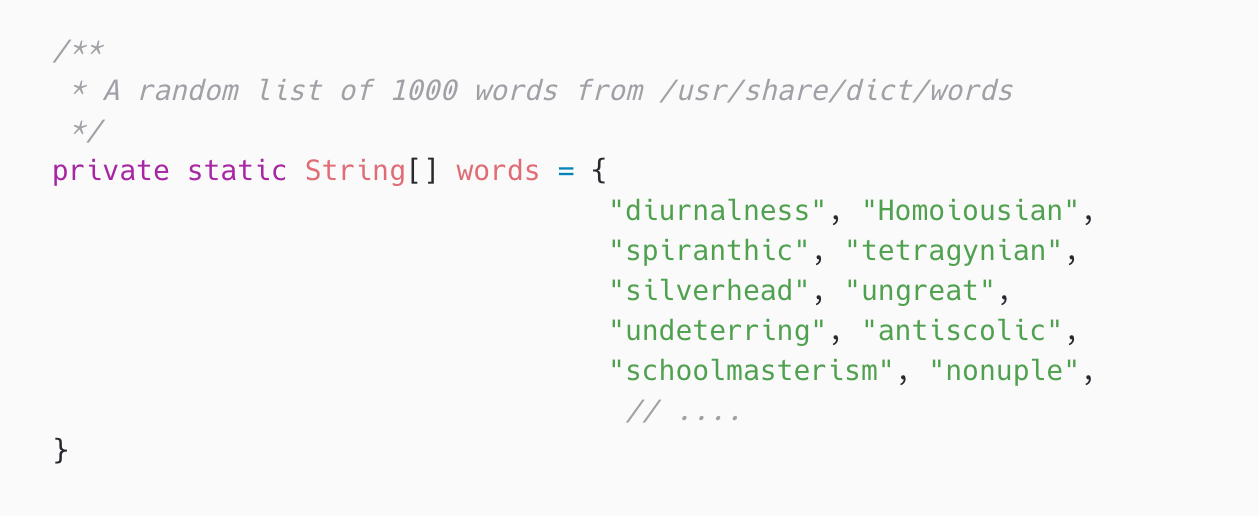
\includegraphics[width=0.85\textwidth]{figures/ch02/contoh-data}
    \caption{Potongan Data pada \textit{Random Text Writer}}
    \label{fig:contoh-data}
\end{figure}


\subsection{Beban Kerja \textit{Word Count}}
\textit{Word Count} adalah algoritma sederhana untuk membaca berkas teks, dan menghitung jumlah kemunculan kata-kata pada file tersebut. Pada algoritma ini, inputnya berupa berkas teks dan outputnya berupa pasangan kata-kata dan jumlah kemunculannya. Beban kerja \textit{word count} akan menghasilkan data keluaran yang lebih kecil dari pada data input seperti pada Gambar \ref{fig:sample-wordcount}.
Karena itu, \textit{word count} memiliki sifat \textit{CPU Bound} yang nantinya akan ditandai dengan tingkat penggunaan CPU yang tinggi dan penggunaan I/O ringan. Selain itu, perilakunya diperkirakan akan tetap sama bahkan pada cluster yang lebih besar.

\begin{figure}[h]
    \centering
    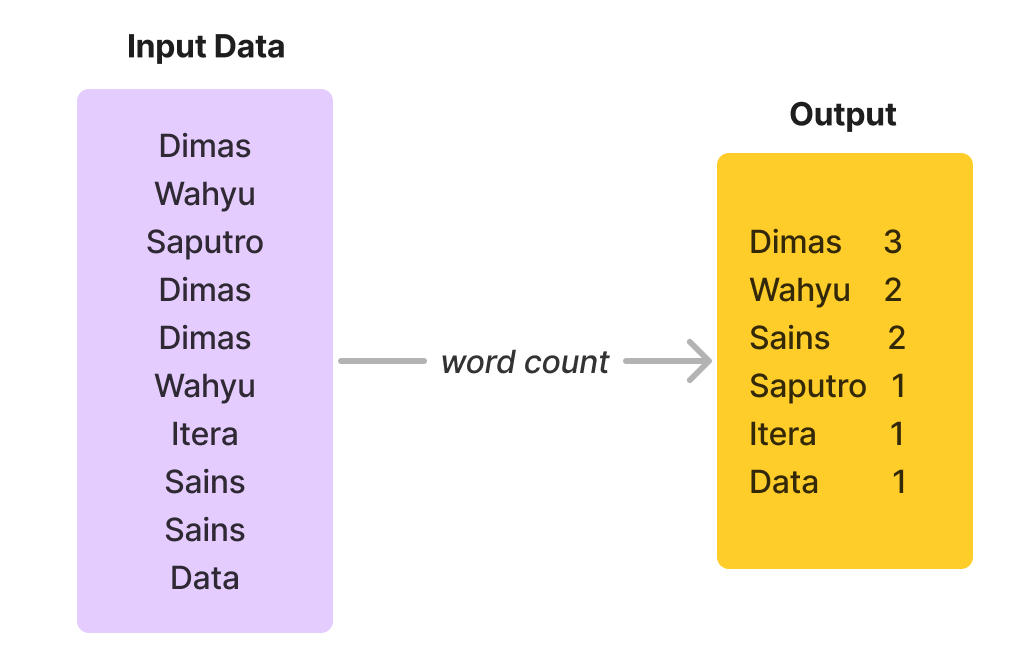
\includegraphics[width=0.7\textwidth]{figures/ch02/sample-wordcount.png}
    \caption{Contoh Input dan Output \textit{Word Count}}
    \label{fig:sample-wordcount}
\end{figure}

Implementasi MapReduce pada \textit{Word Count}\cite{KOMPARASIKECEPATANHADOOP} dapat dilihat pada Gambar \ref{fig:mapreduce-wordcount}. Pada proses MapReduce, data masukan akan melalui beberapa tahapan pemrosesan. Pertama, data akan dipecah menjadi bagian-bagian yang lebih kecil pada proses pemecahan data masukan (\textit{splitting}). Dalam kasus Hadoop MapReduce, data idealnya akan dipecah menjadi beberapa blok berukuran maksimal 128MB.

\begin{figure}[h]
    \centering
    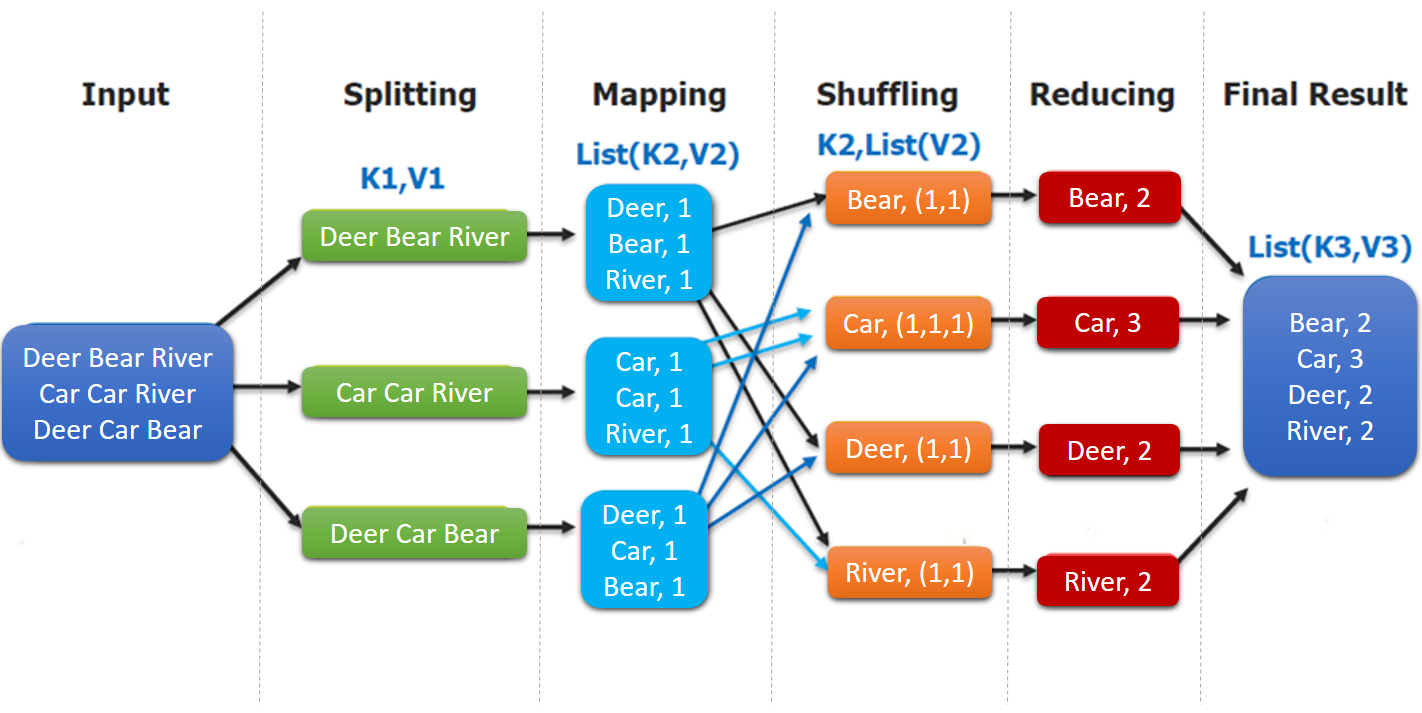
\includegraphics[width=0.85\textwidth]{figures/ch02/map-reduce-word-count-oreilly.png}
    \caption{Implementasi MapReduce pada Word Count \cite{MapReduceDistributedComputing}}
    \label{fig:mapreduce-wordcount}
\end{figure}

Kemudian, blok data tersebut akan diproses lebih lanjut pada tahap pemetaan (\textit{mapping}). Pemetaan merupakan salah satu tahapan terpenting dalam MapReduce. Pada tahap ini, blok data yang sudah dipecah akan diproses untuk menghasilkan pasangan kunci-nilai (\textit{key-value pairs}) sementara, seperti pada contoh kasus \textit{wordcount} yang menghasilkan pasangan kunci-nilai \textit{Dear:1, Bear:1, dan River:1}. Pemetaan dapat melibatkan satu atau beberapa mesin pekerja (\textit{worker}) yang memproses blok data secara paralel.

Selanjutnya adalah tahap pengocokan (\textit{shuffling}) di mana pasangan kunci-nilai hasil pemetaan yang tersebar di beberapa mesin akan dikumpulkan berdasarkan kesamaan kuncinya agar bisa diproses lebih lanjut. Misalnya semua pasangan dengan kunci \textit{Bear} dikumpulkan dalam satu mesin.

Pada tahap terakhir yaitu pengurangan (\textit{reducing}), dilakukan agregasi terhadap pasangan kunci-nilai dengan kunci yang sama untuk menghasilkan keluaran akhir. Seperti pada contoh kasus \textit{wordcount}, pasangan \textit{Bear:1} dan \textit{Bear:1} akan dijumlahkan menjadi \textit{Bear:2} oleh proses pengurangan.

\subsection{Beban Kerja \textit{Sort}}
\textit{Sort} adalah algoritma yang umum digunakan untuk mengurutkan data berdasarkan kriteria tertentu. Algoritma ini menerima data dalam bentuk acak sebagai input, dan menghasilkan data yang terurut sebagai output seperti pada Gambar \ref{fig:sample-sort}. Data input dan output memiliki ukuran yang sama, sehingga beban kerja sort tidak menghasilkan pengurangan data.
Kompleksitas algoritma \textit{sort} bervariasi, tetapi umumnya membutuhkan perbandingan dan pertukaran elemen data yang intensif. Oleh karena itu, beban kerja \textit{sort} cenderung bersifat I/O \textit{bound}, dengan pemanfaatan CPU yang rendah dan penggunaan I/O yang tinggi. 

\begin{figure}[h]
    \centering
    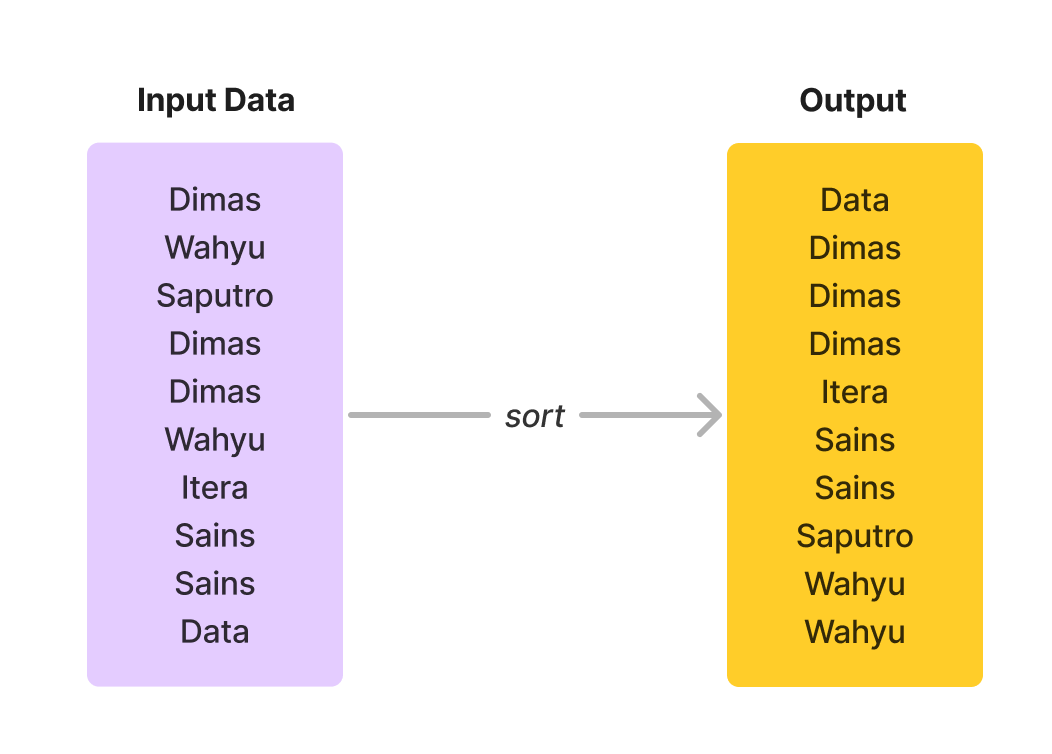
\includegraphics[width=0.7\textwidth]{figures/ch02/sample-sort}
    \caption{Contoh Input dan Output \textit{Sort}}
    \label{fig:sample-sort}
\end{figure}

%\subsection{Word Count - Hadoop}
%\begin{algorithm}[H]
%\caption{Word Count MapReduce}
%\SetKwInOut{Masukan}{Masukan}
%\SetKwInOut{Keluaran}{Keluaran}
%
%\Masukan{Berkas teks dengan setiap baris sebagai kalimat.}
%\Keluaran{Berkas sequence dengan setiap baris sebagai (kata, jumlah).}
%\BlankLine
%\textbf{Tahap Map:}\\
%\For{setiap baris $baris$ dalam teks masukan}{
%    $kata \gets tokenisasi(baris)$\;
%    \For{setiap kata $k$ dalam $kata$}{
%        Keluarkan($k$, 1)\;
%    }
%}
%\BlankLine
%\textbf{Tahap Combine (Opsional):}\\
%\For{setiap pasangan kunci-nilai ($k$, [$j_1, j_2, ..., j_n$])}{
%    $jumlah \gets \sum_{i=1}^{n} j_i$\;
%    Keluarkan($k$, $jumlah$)\;
%}
%\BlankLine
%\textbf{Tahap Reduce:}\\
%\For{setiap pasangan kunci-nilai ($k$, [$j_1, j_2, ..., j_n$])}{
%    $jumlah\_total \gets \sum_{i=1}^{n} j_i$\;
%    Keluarkan($k$, $jumlah\_total$)\;
%}
%\end{algorithm}
%
%\subsection{Word Count - Spark}
%\begin{algorithm}[H]
%\caption{Scala Word Count}
%\SetKwInOut{Masukan}{Masukan}
%\SetKwInOut{Keluaran}{Keluaran}
%
%\Masukan{Berkas teks pada HDFS dengan setiap baris sebagai kalimat.}
%\Keluaran{Berkas teks pada HDFS dengan setiap baris sebagai (kata, jumlah).}
%\BlankLine
%1. Inisialisasi SparkContext\;
%2. $data \gets$ Muat data teks dari HDFS\;
%3. $kata \gets$ Pisahkan setiap baris dalam $data$ menjadi kata-kata individual\;
%4. $pasangan \gets$ Ubah setiap kata menjadi pasangan (kata, 1)\;
%5. $jumlah \gets$ Jumlahkan nilai untuk setiap kata menggunakan `reduceByKey`\;
%6. Simpan $jumlah$ ke HDFS\;
%7. Hentikan SparkContext\;
%\end{algorithm}


%\subsection{Beban Kerja Sort}
%\blindtext

%\subsection{Sort - Hadoop}
%\begin{algorithm}[H]
%\caption{Sort Hadoop MapReduce}
%\SetKwInOut{Masukan}{Masukan}
%\SetKwInOut{Keluaran}{Keluaran}
%
%\Masukan{Data pada HDFS (format dapat ditentukan)}
%\Keluaran{Data terurut pada HDFS (format dapat ditentukan)}
%\BlankLine
%\textbf{Inisialisasi:}\\
%1. Inisialisasi konfigurasi dan JobClient\;
%2. Tentukan jumlah reducer berdasarkan konfigurasi dan kapasitas cluster\;
%3. Tentukan format input, format output, kelas kunci output, dan kelas nilai output (dapat ditentukan pengguna)\;
%4. Buat objek Job dan atur konfigurasi dasar (nama, jar, mapper, reducer, jumlah reducer, format input/output, kelas kunci/nilai output)\;
%5. Atur lokasi input dan output pada HDFS\;
%6. \If{pengguna meminta total-order sort}{
%    Lakukan sampling data input\;
%    Buat berkas partisi untuk total-order sort\;
%    Atur konfigurasi total-order sort pada job\;
%}
%\BlankLine
%\textbf{Tahap Map:}\\
%\For{setiap masukan (kunci, nilai)}{
%    Emit (keluarkan) pasangan (kunci, nilai)\;
%}
%\BlankLine
%\textbf{Tahap Reduce:}\\
%\For{setiap (kunci, [nilai1, nilai2, ...])}{
%    \For{setiap nilai $v$ dalam daftar nilai}{
%        Emit (keluarkan) pasangan (kunci, $v$)\;
%    }
%}
%\BlankLine
%\textbf{Eksekusi:}\\
%7. Cetak informasi job (node, lokasi input/output, jumlah reducer)\;
%8. Jalankan job dan tunggu hingga selesai\;
%9. Cetak waktu eksekusi job\;
%\end{algorithm}

%\subsection{Sort - Spark}
%\begin{algorithm}[H]
%\caption{Scala Sort}
%\SetKwInOut{Masukan}{Masukan}
%\SetKwInOut{Keluaran}{Keluaran}
%
%\Masukan{Berkas teks pada HDFS}
%\Keluaran{Berkas teks terurut pada HDFS}
%\BlankLine
%1. Inisialisasi SparkContext\;
%2. Tentukan jumlah partisi untuk pengurutan\;
%3. $data \gets$ Muat data teks dari HDFS dan ubah setiap baris menjadi pasangan (baris, 1)\;
%4. Buat objek HashPartitioner dengan jumlah partisi yang ditentukan\;
%5. $terurut \gets$ Urutkan $data$ berdasarkan kunci menggunakan `sortByKeyWithPartitioner` dengan HashPartitioner\;
%6. Ambil nilai dari setiap pasangan terurut (yaitu, hanya teks baris)\;
%7. Simpan data terurut $terurut$ ke HDFS\;
%8. Hentikan SparkContext\;
%\end{algorithm}

\section{Data Keluaran HiBench dan Dool}
Diagram pada Gambar \ref{fig:output-hibench-dool} mengilustrasikan data keluaran dari dua alat, yaitu HiBench dan Dool, yang digunakan untuk mengevaluasi kinerja sistem. HiBench berfokus pada pengukuran kinerja keseluruhan dari suatu beban kerja (\textit{benchmark}), sementara Dool memberikan pemantauan sistem yang terperinci secara \textit{real-time}.

\subsection{HiBench \textit{Report}}
HiBench menghasilkan laporan yang mencakup dua metrik utama, yaitu
\begin{enumerate}
	\item \textbf{Waktu Eksekusi (\textit{Execution Time})}: Menunjukkan total waktu yang dibutuhkan untuk menjalankan beban kerja (\textit{benchmark}) dari awal hingga akhir, diukur dalam detik. Nilai detik didapatkan dari \textit{timestamp} awal beban kerja dijalankan, dikurangkan dengan \textit{timestamp} akhir beban kerja.
	\item \textbf{\textit{Throughput}}: Mengukur jumlah data yang diproses per satuan waktu, biasanya dalam bita (\textit{byte}) per detik. Metrik ini mencerminkan efisiensi sistem dalam menangani beban kerja. Ilustrasi \textit{Throughput} terlihat seperti pada Gambar \ref{fig:ilustrasi-throughput}
\end{enumerate}

\begin{figure}[h]
    \centering
    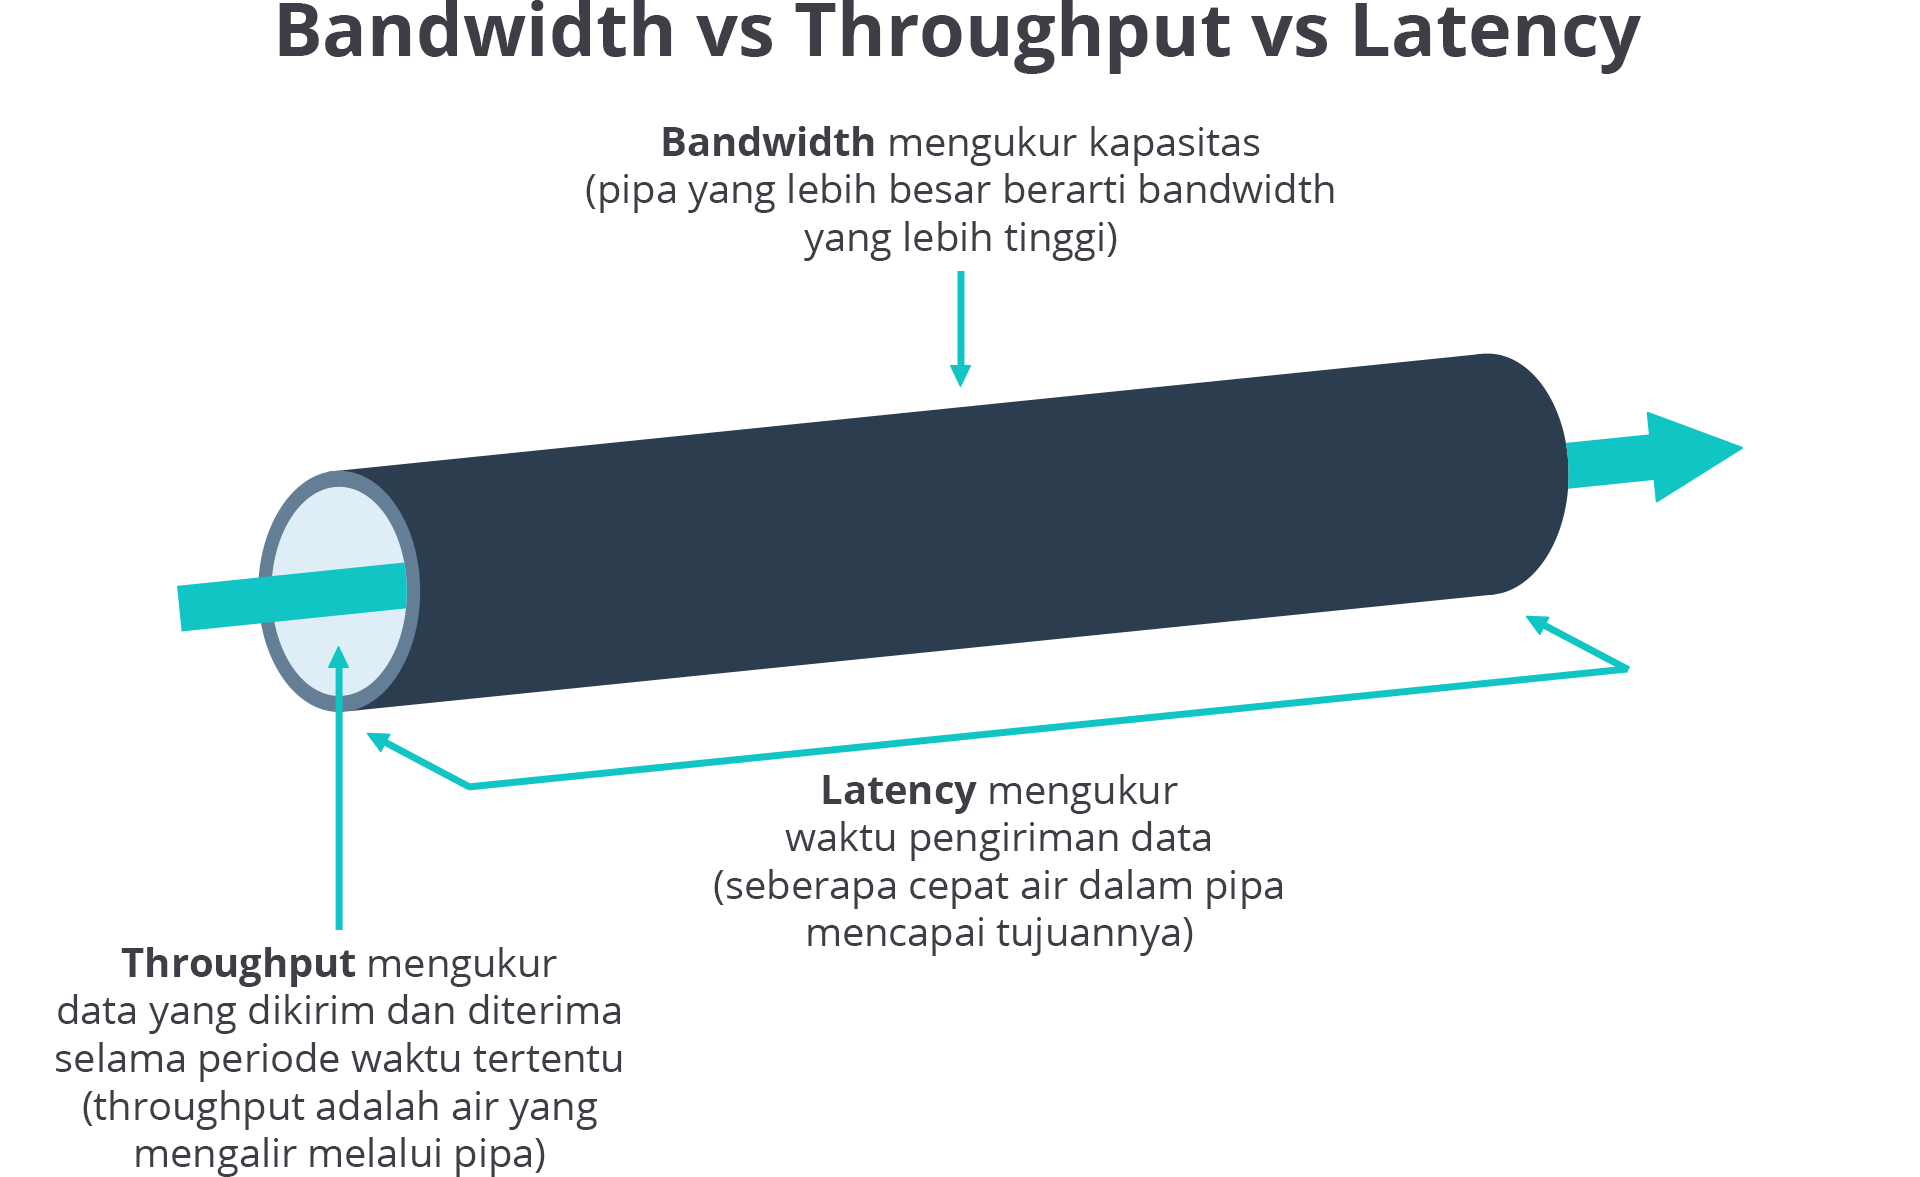
\includegraphics[width=0.7\textwidth]{figures/ch02/ilustrasi-lalu-lintas-jaringan.png}
    \caption{Ilustrasi \textit{Throughput} \cite{PenjelasanApaItu2023}}
    \label{fig:ilustrasi-throughput}
\end{figure}



\subsection{Dool: \textit{System Monitoring}}
Dool menyediakan pemantauan sistem yang mendetail dan diperbarui setiap detik. Data keluaran Dool meliputi berbagai aspek kinerja sistem, antara lain:
\begin{enumerate}
	\item \textbf{\textit{Time}}: \textit{Timestamp} yang menunjukkan waktu pengambilan data.
	\item \textbf{\textit{Date}}: Tanggal pengambilan 
	\item \textbf{\textit{Type}}: Jenis pengukuran yang dilakukan, misalnya CPU, memori, disk, atau jaringan. 
	\item \textbf{io/total}: Total aktivitas input/output (I/O) pada \textit{disk}, diukur dalam jumlah operasi I/O per 
	\item \textbf{total cpu usage}: Persentase penggunaan CPU secara keseluruhan. 
		\begin{enumerate}
		\item \textbf{cpu/user}: Persentase waktu CPU yang digunakan oleh proses-proses di ruang pengguna (\textit{user space}). Ini mencerminkan aktivitas dari aplikasi-aplikasi dan proses-proses yang dijalankan oleh pengguna.
		\item \textbf{cpu/wait}: Persentase waktu CPU yang dihabiskan untuk menunggu operasi I/O selesai. Angka yang tinggi pada metrik ini bisa menunjukkan adanya \textit{bottleneck} pada disk atau jaringan yang menyebabkan CPU harus menunggu data tersedia.
		\end{enumerate}
	\item \textbf{dsk/total}: Total aktivitas \textit{disk}, mencakup baca dan tulis, diukur dalam bita per detik.
		\begin{enumerate}
		\item \textbf{disk/read}: Jumlah data yang dibaca dari disk, diukur dalam bita per detik. Metrik ini penting untuk mengidentifikasi seberapa banyak beban pembacaan yang diterima oleh sistem penyimpanan.
		\item \textbf{disk/write}: Jumlah data yang ditulis ke disk, diukur dalam bita per detik. Metrik ini menunjukkan seberapa banyak data yang sedang ditulis ke penyimpanan, yang bisa mempengaruhi kinerja sistem jika terlalu tinggi.
		\end{enumerate}
	\item \textbf{\textit{memory usage}}: Jumlah memori yang sedang digunakan oleh sistem.
	\item \textbf{net/total}: Total aktivitas jaringan, mencakup data yang dikirim dan diterima, diukur dalam bita per detik.
\end{enumerate}

Akhirnya, HiBench memberikan gambaran umum tentang efisiensi sistem dalam menangani beban kerja tertentu, sementara Dool memungkinkan kita untuk memantau berbagai komponen sistem secara\textit{ real-time} dan mengidentifikasi potensi \textit{bottleneck} atau masalah kinerja.

\begin{figure}[h]
    \centering
    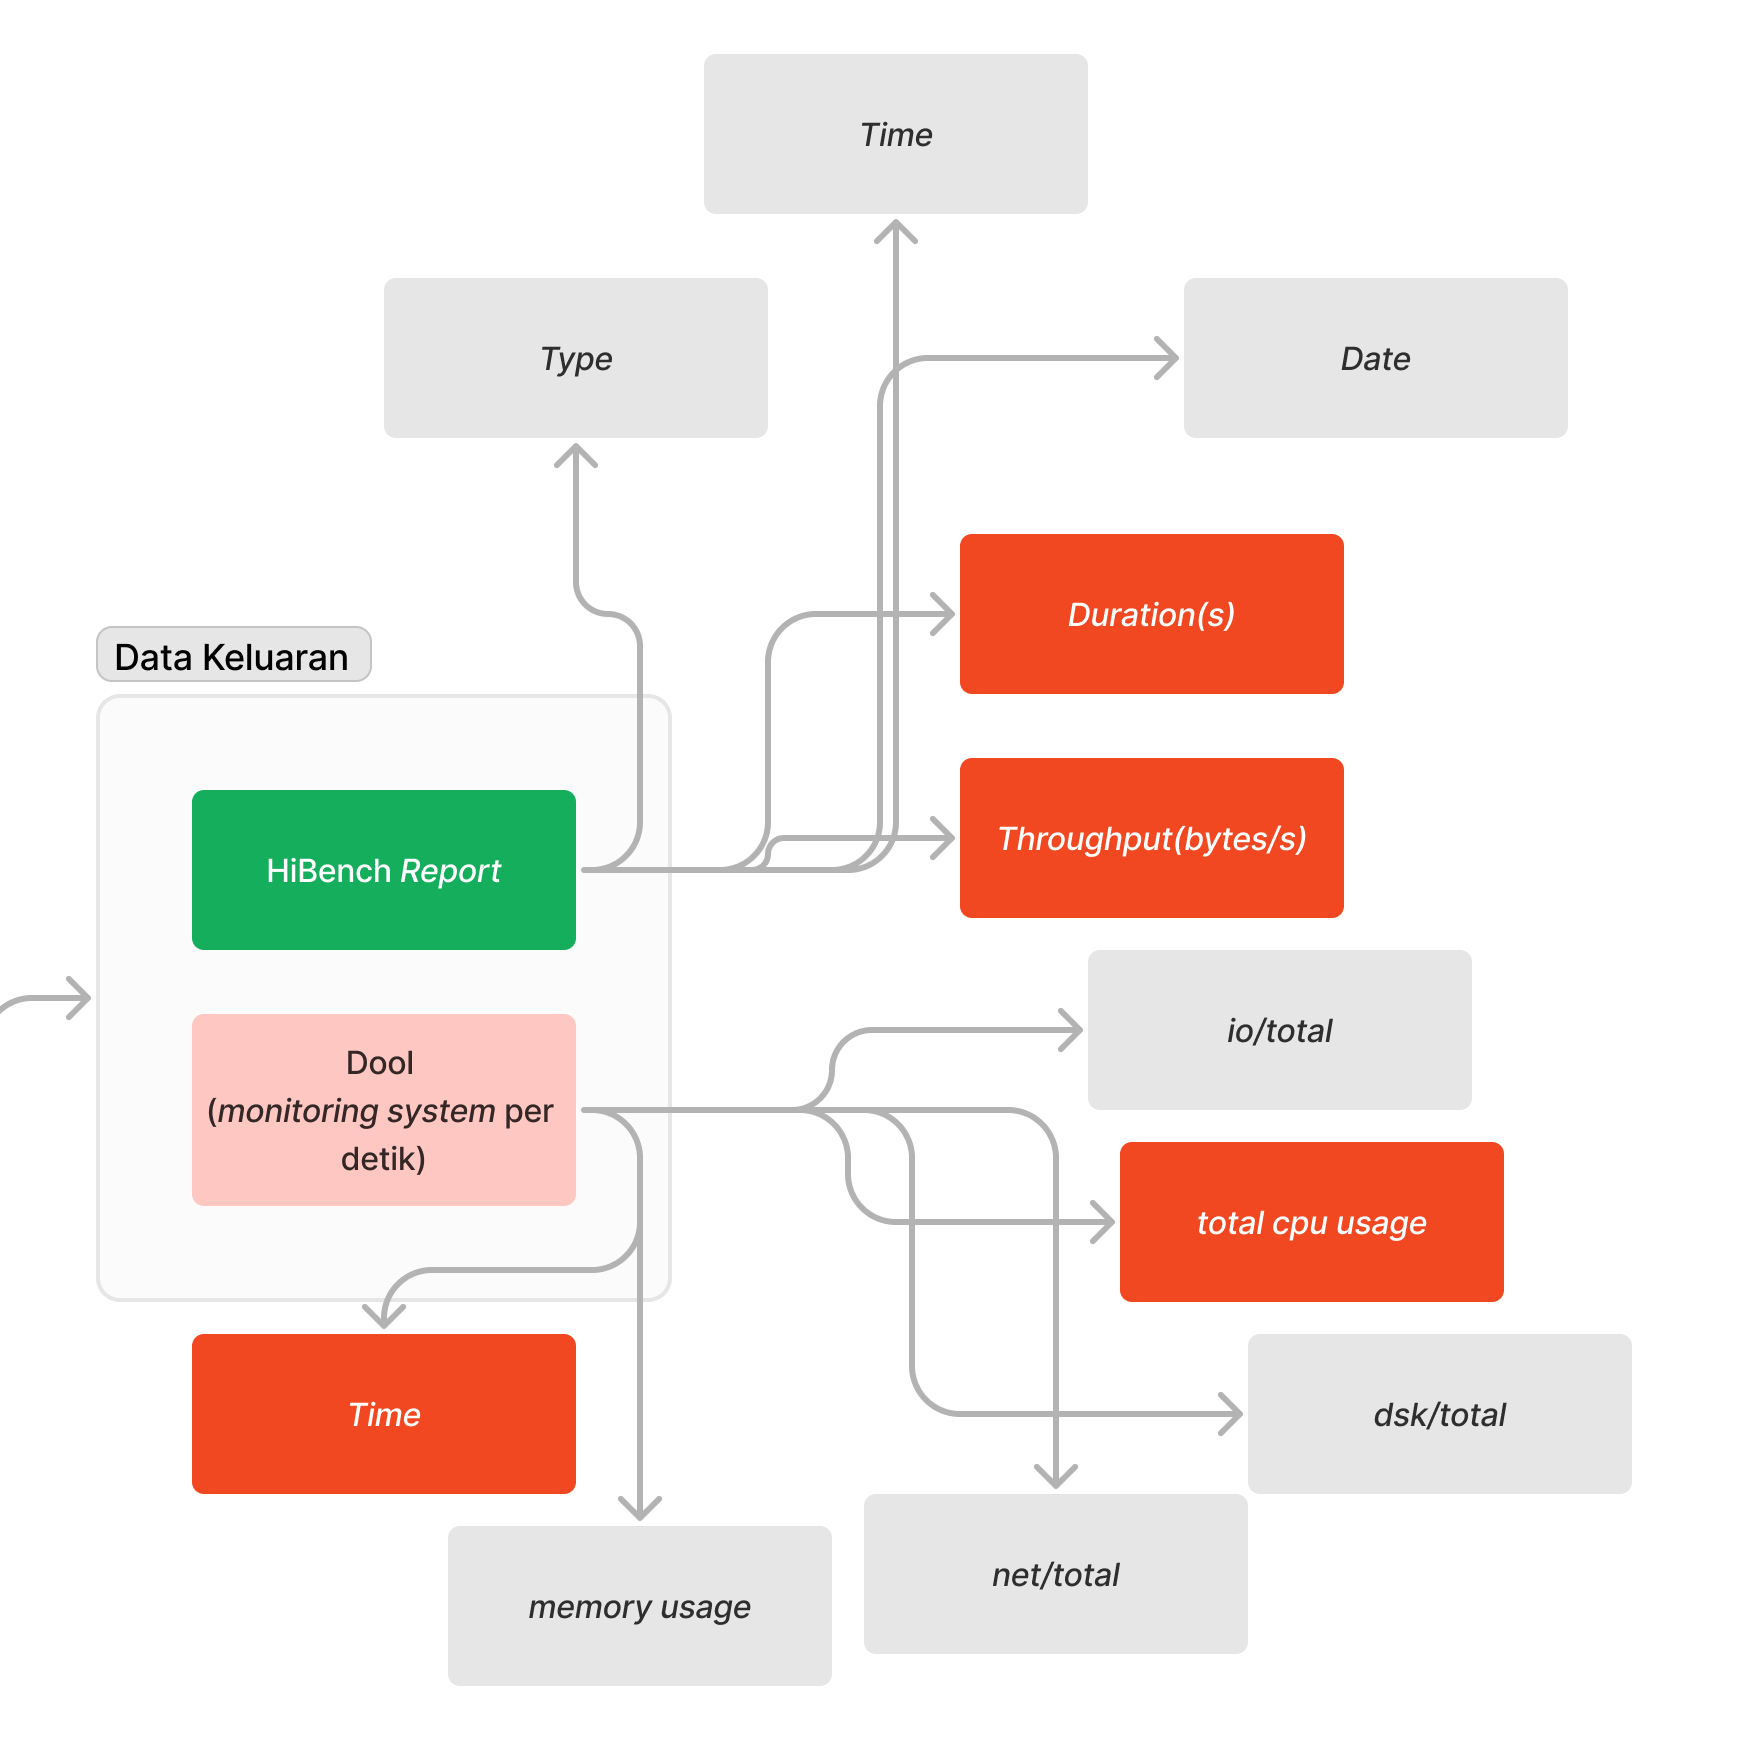
\includegraphics[width=0.9\textwidth]{figures/ch02/output-hibench-dool.png}
    \caption{Data Keluaran HiBench dan Dool}
    \label{fig:output-hibench-dool}
\end{figure}


% Bab 3 metodologi penelitian
\chapter{METODOLOGI PENELITIAN}
%\section{Tempat dan Jadwal Kegiatan Penelitian}
%Dalam melaksanakan sebuah penelitian, perencanaan waktu merupakan komponen kritis yang memastikan alur penelitian dapat berjalan dengan terstruktur dan sistematis. Gambar \ref{fig:jadwal-penelitian} menyajikan jadwal penelitian yang telah dirancang untuk penelitian ini. Jadwal tersebut mencakup rentang waktu mulai dari September 2023 hingga April 2024 dan menguraikan berbagai kegiatan yang akan dilakukan selama periode tersebut. Selanjutnya, penelitian ini akan dilaksanakan di Laboratorium Komputer, Institut Teknologi Sumatera.
%
%\begin{figure}[h!]
%    \centering
%    \includegraphics[width=1\textwidth]{figures/ch03/Timeline-2.png}
%    \caption{Jadwal Penelitian}
%    \label{fig:jadwal-penelitian}
%\end{figure}


\section{Alur Penelitian}
Adapun diagram alir penelitian ini ditunjukkan pada Gambar \ref{fig:diagram alir} terdapat enam tahapan. Langkah awal yang dilakukan pada penelitian ini adalah melakukan identifikasi masalah, yaitu proses mencari, menghimpun, serta menemukan permasalahan yang nantinya akan diselesaikan. Setelah melakukan identifikasi masalah, langkah selanjutnya adalah studi literatur. Studi literatur adalah tahapan untuk mencari solusi dari permasalahan yang sebelumnya sudah kita definisikan. Pencarian solusi ini dapat melalui membaca referensi ilmiah terdahulu, baik melalui jurnal, buku, dokumentasi resmi, tesis, dan lain-lain. Tahapan ini akan memberikan pemahaman mendasar mengenai permasalahan yang sudah didapatkan sebelumnya. 

\begin{figure}[h!]
    \centering
    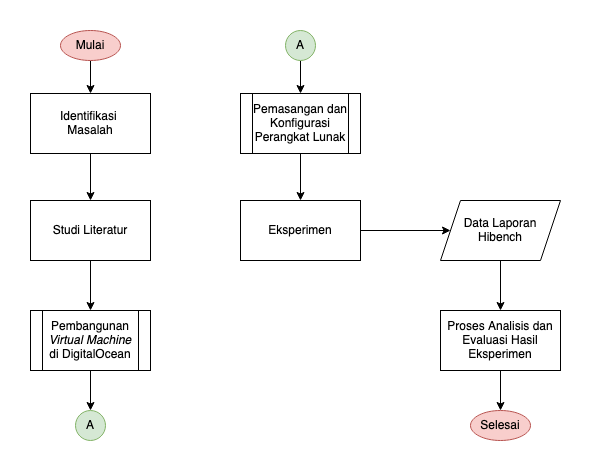
\includegraphics[width=1\textwidth]{figures/ch03/Diagram Tugas Akhir.png}
    \caption{Diagram Alir Penelitian}
    \label{fig:diagram alir}
\end{figure}

Kemudian, penelitian ini akan dilanjutkan pada tahap membangun \textit{virtual machine} di DigitalOcean. DigitalOcean adalah perusahaan penyedia layanan awan \textit{Infrastructure as a Service} (IaaS) yang memberikan banyak pilihan kepada pengguna untuk menggunakan berbagai jenis layanan sesuai dengan kebutuhan, salah satunya yaitu \textit{virtual machine}. \textit{Virtual Machine} tersebut dapat dihentikan atau dihapus kapanpun saat tidak lagi diperlukan. Ketika infrastruktur sudah siap digunakan, penelitian dilanjutkan ke tahap pemasangan perangkat lunak, seperti Hadoop, Spark, dan HiBench. Selanjutnya dilakukan eksperimen pada beban kerja \textit{Micro Benchmarks}. Akhirnya, hasil dari eksperimen akan digunakan untuk proses analisis dan evaluasi.

\section{Penjabaran Langkah Penelitian}
Adapun untuk lebih memperjelas lagi dari setiap langkah yang ada pada Gambar \ref{fig:diagram alir}, dijabarkan secara rinci tahapan-tahapan yang dilakukan pada penelitian ini.

\subsection{Identifikasi Masalah dan Studi Literatur}
Langkah awal penelitian ini adalah identifikasi masalah dan studi literatur. Identifikasi masalah dapat dipahami sebagai tahapan mendefinisikan masalah sehingga masalah tersebut dapat terukur dan jelas untuk dijadikan landasan dalam latar belakang penelitian. Setelah masalah berhasil diidentifikasi, langkah selanjutnya adalah studi literatur yang mana dalam proses ini dilakukan pengumpulan berbagai macam informasi, referensi, dan konsep dasar yang menjadi landasan dasar dari penelitian. Langkah ini dapat dilakukan melalui membaca artikel ilmiah pendukung, buku-buku yang ditulis oleh para ahli, dan jika berkaitan dengan pemrograman dapat melihat dari dokumentasi resmi. Pada tahap ini juga dilakukan analisis terhadap penelitian terdahulu dan dibandingkan dengan identifikasi masalah yang didapatkan untuk membuka celah penelitian baru sehingga penelitian ini dapat bermanfaat. 

\subsection{Membangun \textit{Virtual Machine} di DigitalOcean}
Konfigurasi perangkat keras merupakan aspek penting dalam mengevaluasi kinerja aplikasi \textit{big data} berbasis Hadoop dan Spark. DigitalOcean, sebagai penyedia layanan infrastruktur sebagai layanan (IaaS), memberikan pengguna kebebasan penuh untuk membuat, mengonfigurasi, dan mengelola berbagai infrastruktur yang telah disediakan. Dalam konteks penelitian ini, diperlukan penggunaan mesin virtual, yang dalam DigitalOcean dikenal sebagai "Droplets," yang memungkinkan untuk menyesuaikan berbagai aspek seperti sistem operasi, kapasitas penyimpanan, jumlah prosesor, dan parameter lainnya sesuai dengan kebutuhan spesifik penelitian.

\begin{table}[h!]
	\centering
	\caption{Konfigurasi Perangkat Keras}
	\begin{tabular}{l p{9cm}} 
		\toprule
		\textbf{Nama Parameter}    & \textbf{Nilai Parameter} \\ 
        \midrule
		\textbf{Lokasi Pusat Data} & Singapore - Datacenter 1 - SGP1               \\ 
		\textbf{Sistem Operasi}    & Ubuntu 20.04 (LTS) x64                        \\
		\textbf{Jenis Droplet}     & Basic                                         \\ 
		\textbf{Prosesor}          & Premium AMD - 4 Core                          \\ 
		\textbf{Memori}            & 8 GB                                          \\ 
		\textbf{Penyimpanan}       & 160 GB NVMe SSD                               \\ 
        \bottomrule
	\end{tabular}
	\label{table:conf-hardware}
\end{table}
Penelitian ini mengadopsi mode \textit{pseudo-distributed} yang memungkinkan penggunaan hanya satu \textit{virtual machine} dalam konfigurasi \textit{single node}. Walaupun hanya menggunakan satu \textit{virtual machine}, mode \textit{pseudo-distributed} memungkinkan setiap proses dalam klaster beroperasi secara independen, menciptakan lingkungan di mana semua proses berjalan mandiri satu sama lain. Hal ini memungkinkan untuk lebih berfokus pada pengumpulan data dan analisis, tanpa perlu melakukan konfigurasi yang rumit terkait dengan pengaturan klaster. Spesifikasi perangkat keras yang digunakan untuk \textit{virtual machine} dalam mode \textit{pseudo-distributed} sesuai pada Tabel \ref{table:conf-hardware}. Penjelasan lengkap tentang pembuatan \textit{virtual machine} (VM) pada \textit{platform} DigitalOcean dan cara mengakses VM tersebut disajikan pada Lampiran \ref{appendix:A}.

\subsection{Pemasangan dan Konfigurasi Perangkat Lunak}
Pemasangan dan konfigurasi perangkat lunak merupakan hal yang krusial dalam penelitian ini. Perangkat lunak yang diperlukan ditunjukkan pada Tabel \ref{table:software-needs}.

\begin{table}[h]
	\centering
	\caption{Perangkat Lunak yang Dibutuhkan}
		\begin{tabular}{l p{9cm}} 
		\toprule
			\textbf{Perangkat Lunak} & \multicolumn{1}{c}{\textbf{Deskripsi}}                                                                                \\ 
            \midrule
			Ubuntu 20.04 LTS x64     & Sistem operasi Linux berbasis Ubuntu  \\ 
			Git                      & Sistem kontrol versi untuk mengelola perubahan dalam kode sumber perangkat lunak                                       \\
			Maven                    & Perangkat lunak manajemen proyek Java                            \\ 
			Java 8                   & \multirow{3}{*}{Bahasa pemrograman dasar}                                 \\ 
			Python 3.7               &                                                                                                                        \\
			Scala 2.11.8               &                                                                                                                        \\
			Hadoop 2.4                & Perangkat lunak pengolahan data terdistribusi untuk penyimpanan dan manajemen data besar                               \\ 
			Spark 2.1.3               & Kerangka kerja pemrosesan data terdistribusi yang berjalan di atas Hadoop                                              \\ 
			Hibench   & Alat yang digunakan untuk mengukur kinerja Hadoop dan Spark                                                            \\
			Dool   & Alat untuk melihat penggunaan \textit{resource} sistem                                                             \\
            \bottomrule 
		\end{tabular}
	\label{table:software-needs}
\end{table}


Alur kerja instalasi perangkat lunak dalam penelitian ini dapat dilihat pada Gambar \ref{fig:alurkerja-soft}. Pada gambar, terdapat tiga bagian utama, yaitu \textit{prerequisites} (perangkat lunak prasyarat) ditandai dengan warna biru, alat penyimpanan dan pemrosesan \textit{Big Data} ditandai dengan warna oren, dan alat untuk mengukur kinerja \textit{big data} ditandai dengan warna hijau. Semua perangkat lunak dijalankan pada sistem operasi Ubuntu 20.04 LTS x64.\\

\begin{landscape}
\begin{figure}[h]
    \centering
    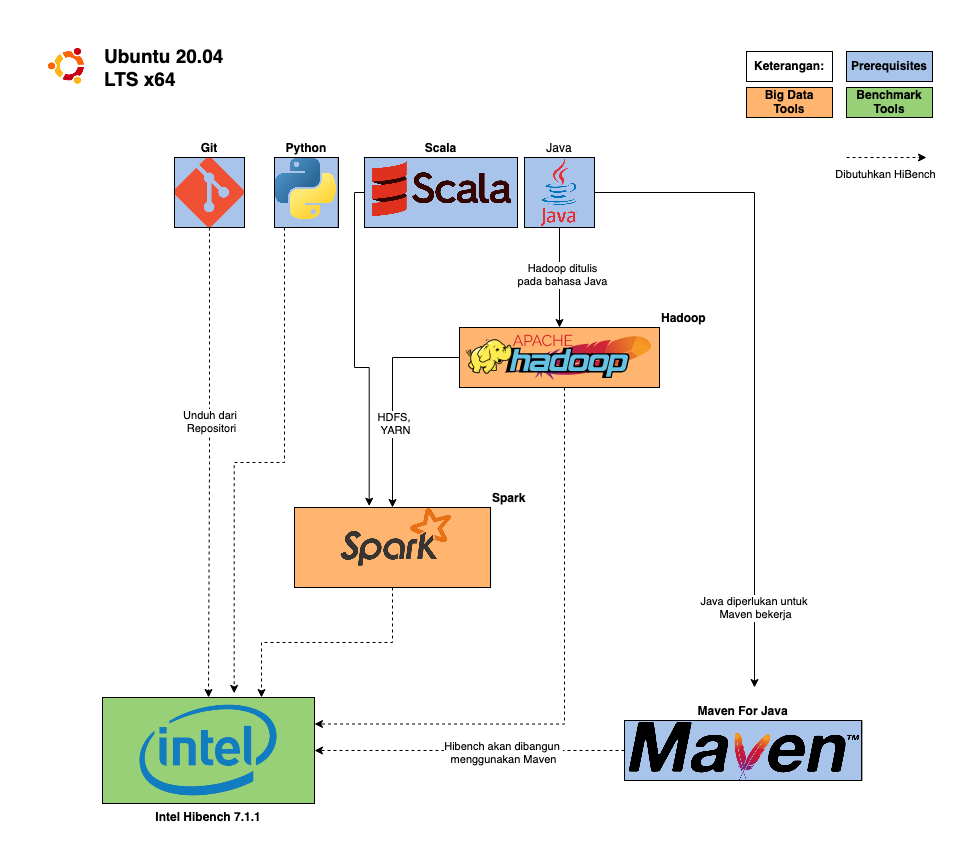
\includegraphics[height=0.65\linewidth]{figures/ch03/alurkerja-soft.png}
    \caption{Alur Instalasi Perangkat Lunak}
    \label{fig:alurkerja-soft}
\end{figure}
\end{landscape}

\textbf{Instalasi Perangkat Lunak Prasyarat}\\
Ada beberapa perangkat lunak yang perlu diimplementasikan sebelum memasang Hadoop, Spark, dan HiBench, yaitu:
\begin{enumerate}
	\item Ubuntu 20.04 LTS x64
	\item Git
	\item Java 8 dan Maven
	\item Python 3.7
	\item Scala 2.11.8
\end{enumerate}

Pemasangan dan konfigurasi perangkat lunak pada tahapan ini tidak membutuhkan urutan. Akan tetapi, pada penelitian ini dibuatkan alur untuk pemasangan dan konfigurasi perangkat lunak prasyarat seperti pada Gambar \ref{fig:prasyarat-flow}. Penjelasan lengkap mengenai tata cara instalasi dan konfigurasi perangkat lunak prasyarat ini disajikan pada Lampiran \ref{appendix:B}. \\

\begin{figure}[h!]
    \centering
    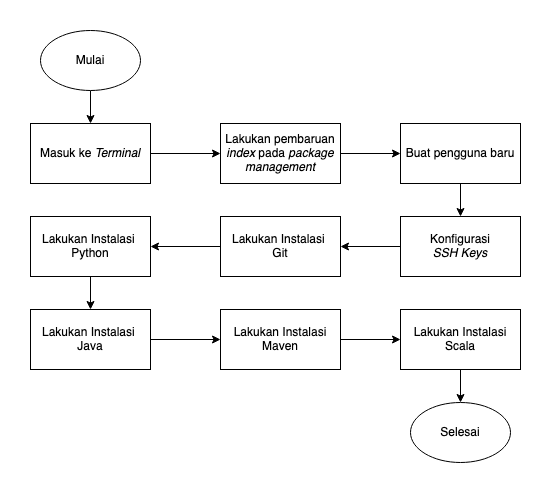
\includegraphics[width=0.9\textwidth]{figures/ch03/prasayarat-flow.png}
    \caption{Alur Instalasi Perangkat Lunak Prasyarat}
    \label{fig:prasyarat-flow}
\end{figure}

\textbf{Instalasi dan Konfigurasi Hadoop}\\
Hadoop adalah perangkat lunak \textit{open source} yang efektif dalam menyimpan dan memproses data dalam skala besar. Daripada menggunakan satu komputer besar untuk menyimpan dan memproses data, Hadoop memungkinkan pengklasteran beberapa komputer untuk menganalisis set data besar secara paralel dengan lebih cepat. Ada beberapa perangkat lunak prasyarat yang perlu dipasang sebelum menggunakan Hadoop. Setelah perangkat lunak prasyarat berhasil dipasang, Hadoop juga dapat dipasang mengikuti panduan lengkap pada Lampiran \ref{appendix:C}. 
Secara umum, alur yang harus dilakukan meliputi pengunduhan berkas Hadoop. Selanjutnya akan dilakukan pengubahan kepemilikan berkas ke \textit{user hdfsuser}. Karena Hadoop tidak mendukung IPv6, maka fitur ini perlu dimatikan juga. Alur pemasangan dan konfigurasi Hadoop lebih jelas sesuai dengan Gambar \ref{fig:hadoop-flow}.\\

\begin{figure}[h!]
    \centering
    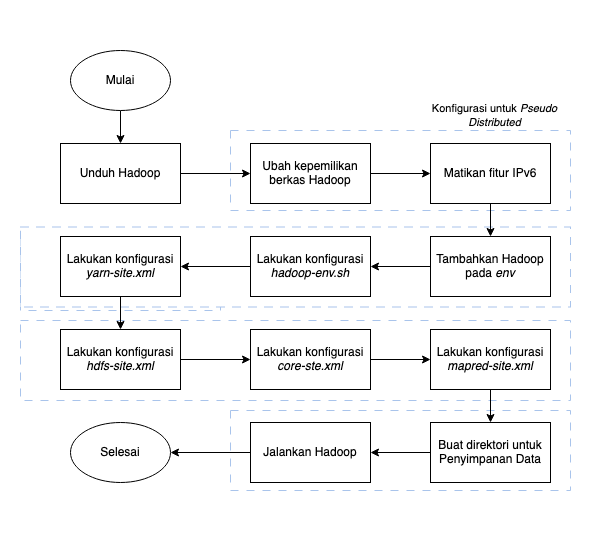
\includegraphics[width=0.9\textwidth]{figures/ch03/hadoop-flow.png}
    \caption{Alur Instalasi dan Konfigurasi Hadoop}
    \label{fig:hadoop-flow}
\end{figure}

\textbf{Instalasi dan Konfigurasi Spark}\\
Apache Spark adalah sebuah kerangka kerja pengolahan data terdistribusi yang sangat cepat dan efisien. Spark dan Hadoop memiliki hubungan yang erat. Spark dapat berjalan di atas \textit{Hadoop Distributed File System} (HDFS) dan dapat menggunakan Hadoop YARN sebagai manajer sumber daya. Oleh karena itu, instalasi Spark membutuhkan Hadoop sudah terpasang lebih dahulu. Alur pemasangan dan konfigurasi spark terlihat seperti pada Gambar \ref{fig:spark-flow}. Apabila Hadoop sudah berhasil terpasang, langkah selanjutnya adalah memasang Spark seperti pada Lampiran \ref{appendix:D}.\\

\begin{figure}[h]
    \centering
    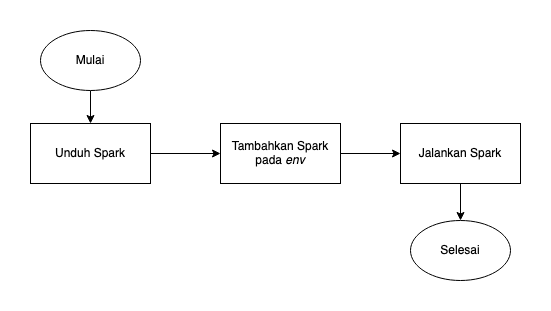
\includegraphics[width=0.7\textwidth]{figures/ch03/spark-flow.png}
    \caption{Alur Instalasi dan Konfigurasi Spark}
    \label{fig:spark-flow}
\end{figure}

\textbf{Instalasi dan Konfigurasi HiBench}\\
Sebelum melakukan eksperimen, diperlukan suatu perangkat lunak pengukuran kinerja sistem \textit{Big Data}, yaitu HiBench. HiBench tidak dapat digunakan secara langsung ketika sudah berhasil diunduh, melainkan harus dilakukan pembangunan beberapa modul yang dibutuhkan dengan Maven dan konfigurasi beberapa parameter. 

\begin{figure}[h]
    \centering
    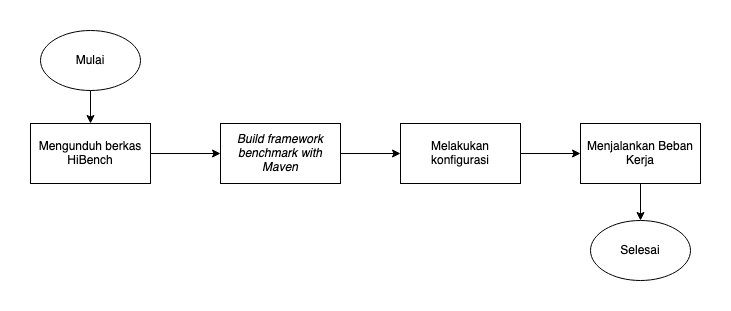
\includegraphics[width=0.9\textwidth]{figures/ch03/hibench-flow.png}
    \caption{Alur Instalasi dan Konfigurasi HiBench}
    \label{fig:hibench-flow}
\end{figure}

Secara umum, alur instalasi dan konfigurasi HiBench sesuai dengan Gambar \ref{fig:hibench-flow}. Berkas HiBench diunduh dari repositori, dilanjutkan dengan pembangunan beberapa modul yang nantinya dibutuhkan. Selanjutnya, dilakukan konfigurasi beberapa berkas seperti \textit{hibench.conf}, hadoop.conf, dan spark.conf. Jika telah dilakukan konfigurasi, dapat dilanjutkan dengan menjalankan beban kerja atau eksperimen. Lebih lanjut, pemasangan dan konfigurasi HiBench dijelaskan pada Lampiran \ref{appendix:E}.

%\begin{table}[]
%\caption{Konfigurasi \textit{HiBench}}
%\label{table:conf-hibench}
%\scriptsize
%\centering
%\begin{tabular}{ll}
%\hline
%\multicolumn{1}{c}{Nama Parameter}  & \multicolumn{1}{c}{Nilai} \\ \hline
%hibench.default.map.parallelism     & 8                         \\
%hibench.default.shuffle.parallelism & 8 \\ \hline                        
%\end{tabular}
%\end{table}


\subsection{Eksperimen}
Setelah instalasi dan konfigurasi perangkat keras dan perangkat lunak berhasil diselesaikan, tahap selanjutnya adalah eksperimen. Tahap ini melibatkan serangkaian pengujian yang terkontrol untuk mengevaluasi kinerja \textit{platform big data} Hadoop dan Spark dalam menjalankan beban kerja tertentu dengan berbagai ukuran data. Tujuan utama eksperimen ini adalah untuk menjawab pertanyaan penelitian yang telah didefinisikan sebelumnya dan memperoleh pemahaman yang komprehensif tentang karakteristik kinerja masing-masing \textit{platform}.

Penelitian ini difokuskan pada pengujian dua beban kerja yang umum dalam pemrosesan big data, yaitu \textit{word count} dan \textit{sort}. Beban kerja ini akan dieksekusi pada dua \textit{platform big data} yang populer, yaitu Hadoop dan Spark. Setiap kombinasi \textit{platform} dan beban kerja akan diuji dengan 12 ukuran data yang berbeda, mulai dari 100 KB hingga 15 GB. Detail ukuran data yang digunakan ditunjukkan pada Tabel \ref{table:variasi-input-data}. Untuk memastikan reliabilitas dan konsistensi hasil, setiap kombinasi \textit{platform}, beban kerja, dan ukuran data akan diulang sebanyak 5 kali. 

Proses eksperimen menghasilkan dua jenis berkas data: 
\begin{enumerate}
	\item \textit{HiBench Report}: Berisi informasi tentang kinerja beban kerja, termasuk waktu eksekusi, dan \textit{throughput}.
	\item \textit{Dool System Monitoring}: Berisi informasi detail tentang aktivitas sistem selama eksekusi beban kerja, seperti penggunaan CPU, memori, I/O \textit{disk}, dan jaringan.
\end{enumerate}

Secara keseluruhan, desain eksperimen ini menghasilkan 240 percobaan individu, seperti yang diilustrasikan pada Gambar \ref{fig:total-percobaan}. Setiap percobaan mewakili kombinasi unik dari:
\begin{enumerate}
	\item \textit{Platform big data} (Hadoop atau Spark)
	\item Beban kerja (\textit{word count} atau \textit{sort*})
	\item Ukuran data (12 variasi)
	\item Pengulangan (5 kali)
\end{enumerate}

\begin{figure}[h]
    \centering
    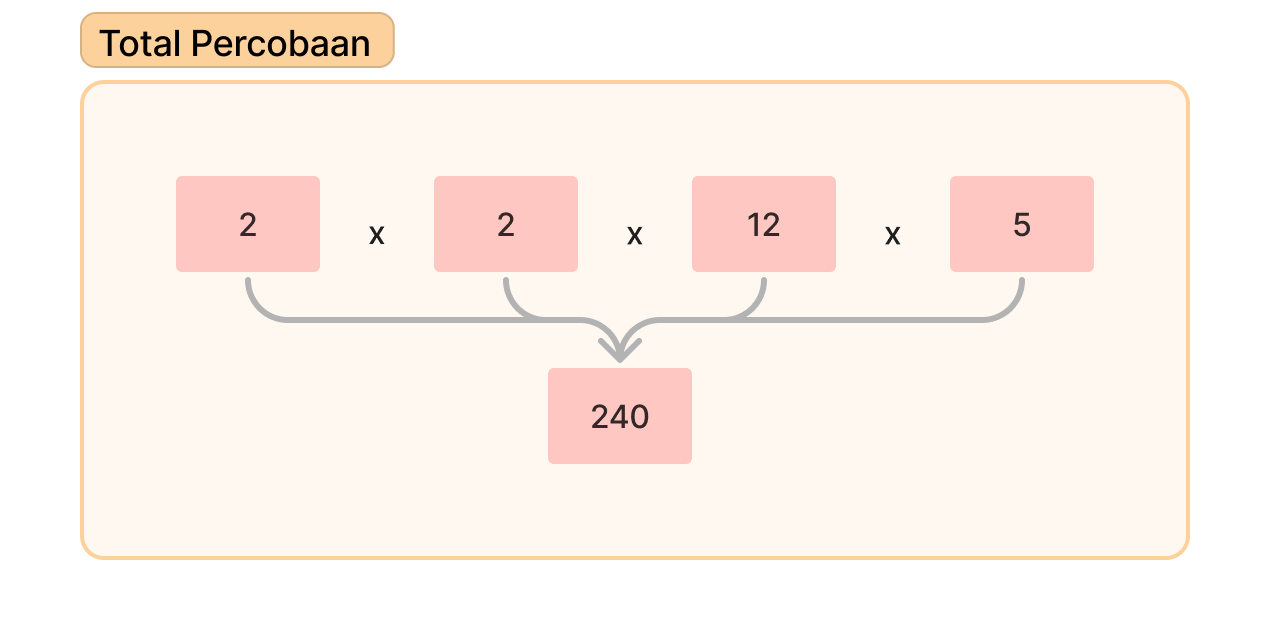
\includegraphics[width=0.7\textwidth]{figures/ch03/total-percobaan.png}
    \caption{Total Percobaan}
    \label{fig:total-percobaan}
\end{figure}

\begin{landscape}
\begin{figure}[h]
    \centering
    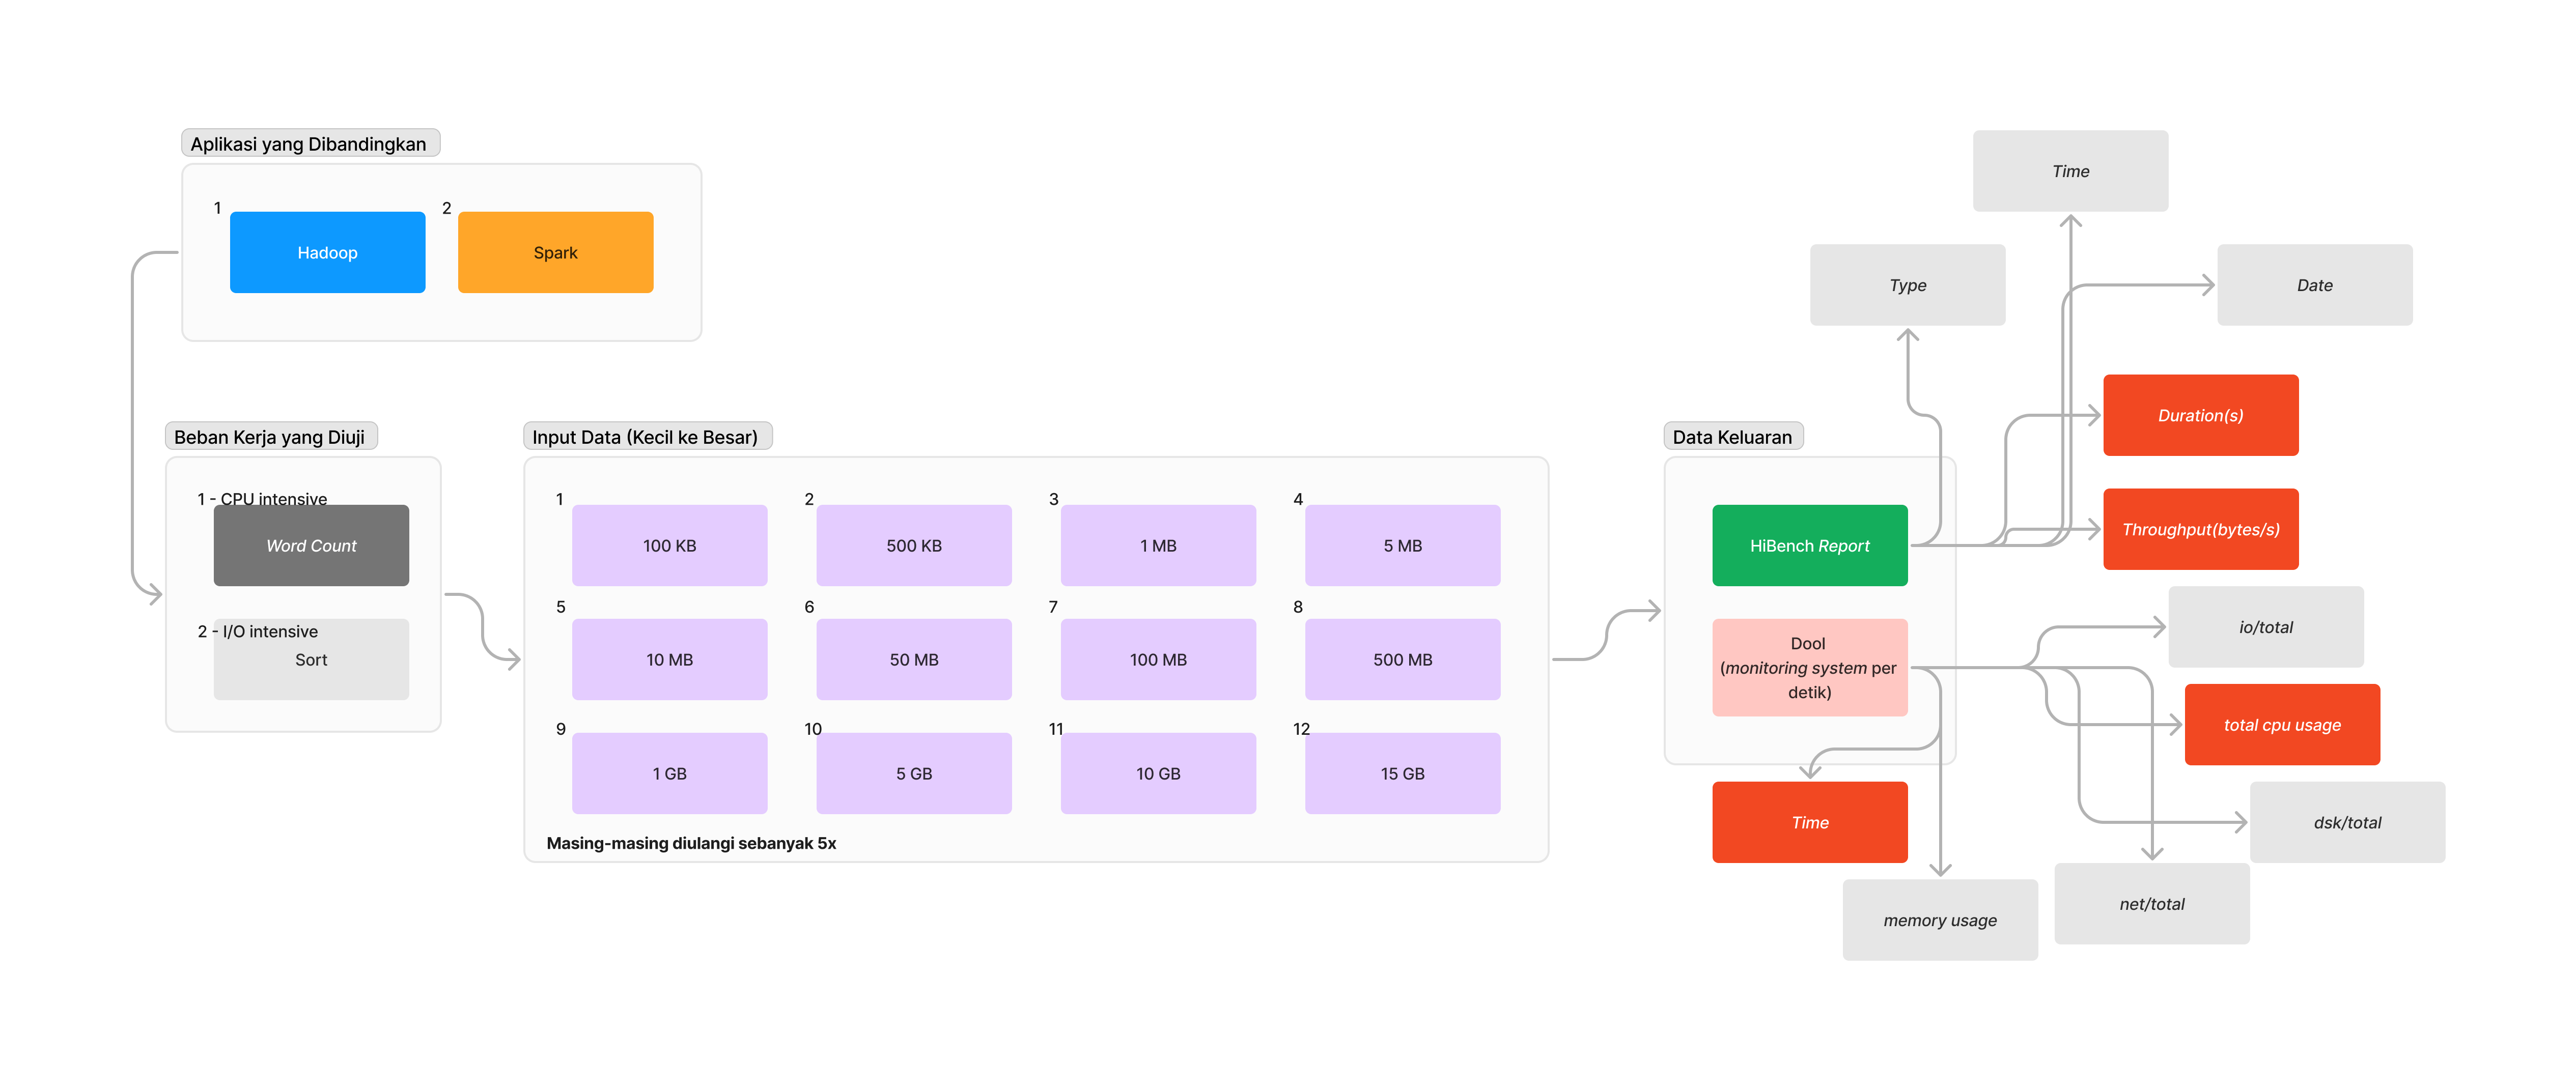
\includegraphics[width=\linewidth, height=0.5\linewidth]{figures/ch03/flow-penelitian-umum.png}
    \caption{\textit{End-to-end} Penelitian}
    \label{fig:flow-penelitian-umum}
\end{figure}
\end{landscape}

Sebagai contoh, untuk \textit{platform} Hadoop dengan beban kerja \textit{word count} dan ukuran data 100 KB, akan menghasilkan 5 HiBench \textit{Report} dan 5 berkas Dool \textit{System Monitoring}, sesuai dengan jumlah pengulangan.  Ilustrasi ini dapat dilihat pada Gambar \ref{fig:contoh-percobaan}.

\begin{figure}[h]
    \centering
    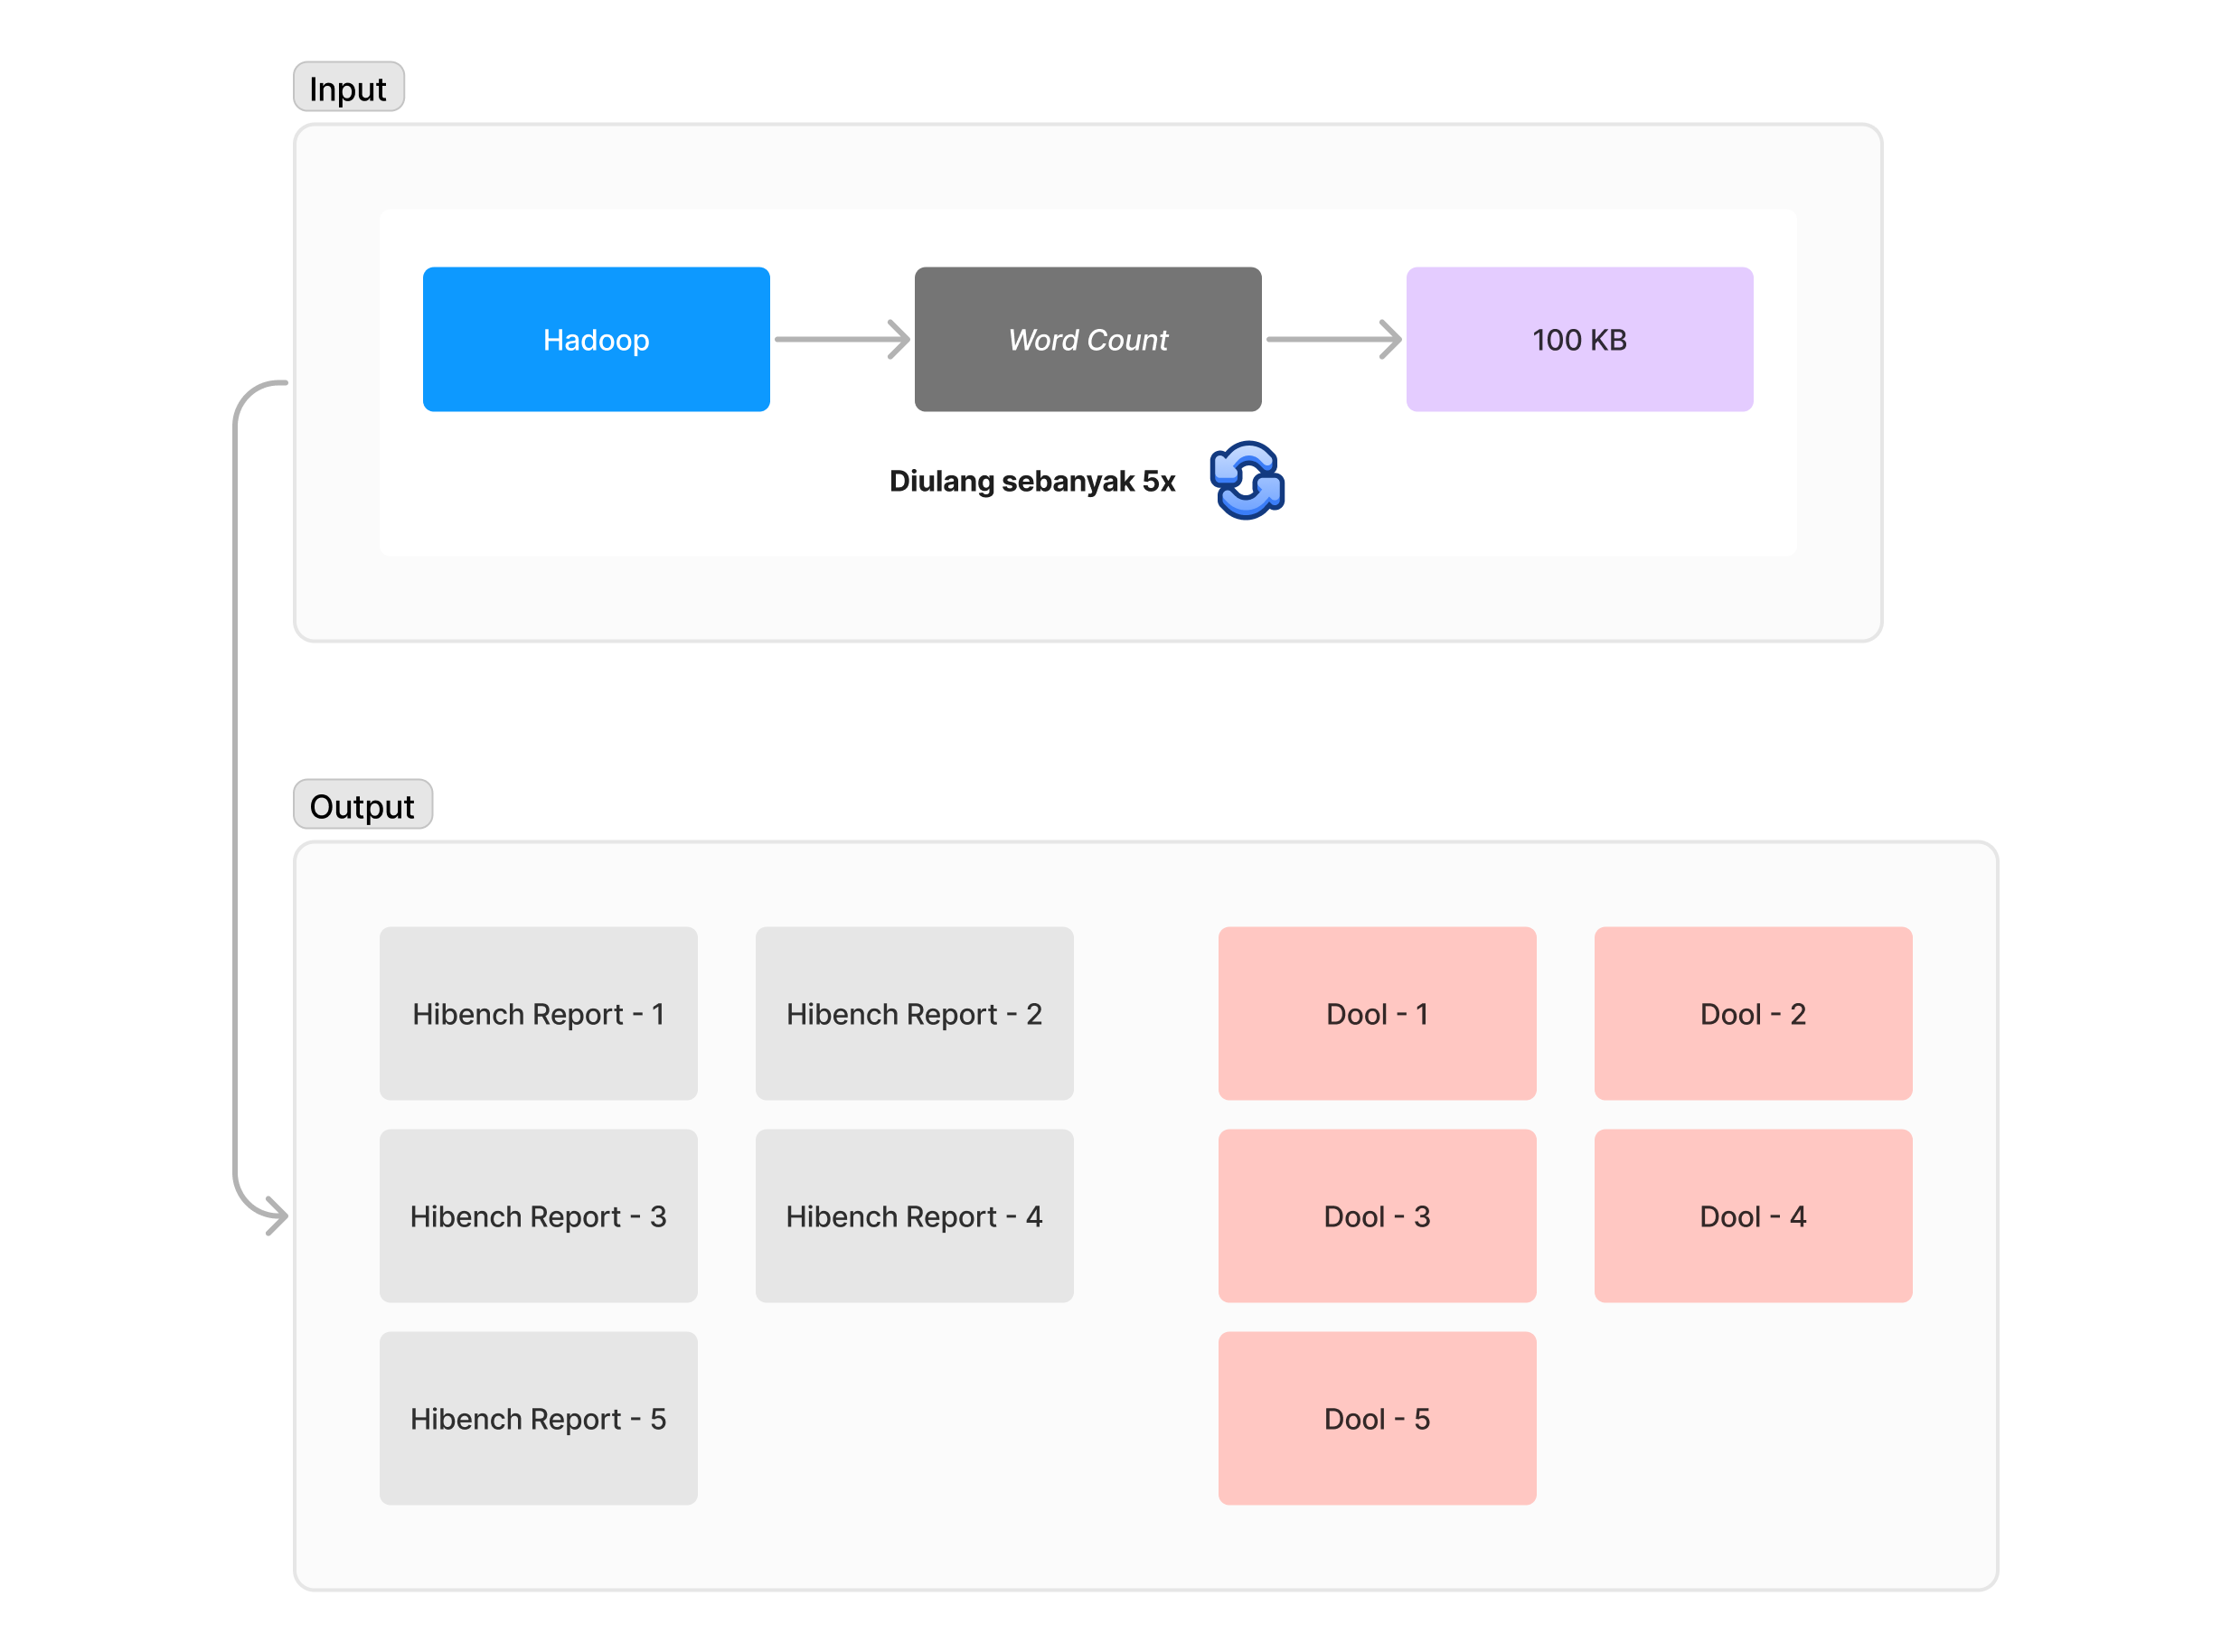
\includegraphics[width=0.9\textwidth]{figures/ch03/contoh-percobaan.png}
    \caption{Contoh Percobaan}
    \label{fig:contoh-percobaan}
\end{figure}

\begin{table}[]
\caption{Variasi Input Data}
\label{table:variasi-input-data}
\centering
\begin{tabular}{lll}
\hline
\multicolumn{1}{c}{No} & \multicolumn{1}{c}{Label Input Data} & \multicolumn{1}{c}{\begin{tabular}[c]{@{}c@{}}Ukuran Input Data  (bita)\end{tabular}} \\ \hline
1  & 100 KB & 100000 ($1 * 10^5$) \\
2  & 500 KB & 500000 ($5 * 10^5$) \\
3  & 1 MB   & $1 * 10^6$          \\
4  & 5 MB   & $5 * 10^6$          \\
5  & 10 MB  & $1 * 10^7$          \\
6  & 50 MB  & $5 * 10^7$          \\
7  & 100 MB & $1 * 10^8$          \\
8  & 500 MB & $5 * 10^8$          \\
9  & 1 GB   & $1 * 10^9$          \\
10 & 5 GB   & $5 * 10^9$          \\
11 & 10 GB  & $1 * 10^10$         \\ 
12 & 15 GB  & $1.5 * 10^10$       \\ \hline
\end{tabular}
\end{table}


Karena jumlah percobaan yang banyak, otomatisasi menjadi penting untuk memastikan efisiensi dan akurasi.  Skrip khusus dikembangkan untuk mengotomatiskan seluruh proses eksperimen, termasuk konfigurasi HiBench, persiapan data, eksekusi beban kerja, dan pengumpulan data. Detail skrip otomatisasi dapat ditemukan pada Lampiran \ref{appendix:F}.

Algoritma otomatisasi eksperimen dimulai dengan mengubah direktori kerja ke direktori HiBench.  Selanjutnya, algoritma melakukan iterasi untuk setiap beban kerja yang ditentukan.  Di dalam setiap iterasi beban kerja, dilakukan iterasi lagi untuk setiap ukuran data.  Pada setiap kombinasi beban kerja dan ukuran data, konfigurasi HiBench diubah sesuai dengan ukuran data yang dipilih.

Skrip persiapan data Hadoop dan Spark dijalankan berulang kali hingga proses persiapan berhasil.  Setelah data siap, perulangan dilakukan sebanyak jumlah pengulangan yang ditentukan.  Dalam setiap perulangan, perangkat lunak "dool" diaktifkan untuk memonitor aktivitas sistem, \textit{benchmark} Hadoop atau Spark dijalankan, dan monitoring sistem dihentikan.

Setelah semua perulangan selesai, algoritma menunggu selama 15 detik sebelum melanjutkan ke ukuran data berikutnya. Proses ini berlanjut hingga semua kombinasi beban kerja dan ukuran data selesai diproses.

\subsection{Analisis dan Evaluasi Hasil Eksperimen}

Setelah menyelesaikan 240 percobaan yang dijelaskan di bagian eksperimen, langkah selanjutnya adalah menganalisis dan mengevaluasi hasil yang diperoleh. Analisis ini bertujuan untuk menjawab pertanyaan penelitian dan memahami bagaimana kinerja Hadoop dan Spark dalam menjalankan beban kerja \textit{word count} dan \textit{sort} dengan berbagai ukuran data. Berikut adalah beberapa aspek yang akan dikaji:

\begin{enumerate}	
	\item \textbf{Kinerja}
	\begin{enumerate}
		\item \textbf{Persebaran Waktu Eksekusi pada Hadoop dan Spark}. Bagian ini akan menganalisis sebaran waktu eksekusi untuk setiap beban kerja (\textit{word count} dan \textit{sort*}) pada kedua aplikasi (Hadoop dan Spark) dengan berbagai ukuran data. Analisis ini akan membantu memahami variabilitas kinerja dan konsistensi hasil pada setiap kombinasi aplikasi, beban kerja, dan ukuran data.
		\item \textbf{Persebaran \textit{Throughput} pada Hadoop dan Spark}. Mirip dengan analisis waktu eksekusi, persebaran \textit{throughput} juga akan dianalisis untuk setiap kombinasi aplikasi, beban kerja, dan ukuran data. Throughput, yang menunjukkan jumlah data yang diproses per satuan waktu,  merupakan metrik penting dalam evaluasi kinerja sistem big data.  Visualisasi distribusi throughput akan membantu dalam memahami efisiensi pemrosesan data oleh Hadoop dan Spark.
		\item \textbf{Rata-rata Waktu Eksekusi pada Hadoop dan Spark}. Selain persebaran, rata-rata waktu eksekusi untuk setiap kombinasi akan dihitung dan dibandingkan.  Ini memberikan gambaran umum tentang kinerja relatif setiap aplikasi dalam menyelesaikan beban kerja tertentu dengan ukuran data tertentu. Perbedaan rata-rata waktu eksekusi antara Hadoop dan Spark, serta tren perubahannya seiring dengan peningkatan ukuran data, akan diidentifikasi dan dibahas.
		\item \textbf{Rata-rata \textit{Throughput} pada Hadoop dan Spark}. Serupa dengan rata-rata waktu eksekusi, rata-rata \textit{throughput} juga akan dihitung dan dibandingkan untuk setiap kombinasi. Analisis ini membantu memahami bagaimana efisiensi pemrosesan data berubah dengan berbagai beban kerja dan ukuran data, serta memberikan wawasan tentang skalabilitas setiap platform.
		\item \textbf{\textit{Rate of Change}}. \textit{Rate of Change} akan dihitung untuk metrik-metrik kinerja seperti waktu eksekusi dan throughput. Ini akan menunjukkan seberapa besar perubahan kinerja seiring dengan peningkatan ukuran data.  
	\end{enumerate}
	\item \textbf{Penggunaan Sumber Daya}
	\begin{enumerate}
	\item \textbf{Penggunaan CPU}. Bagian ini akan menganalisis penggunaan CPU oleh Hadoop dan Spark selama menjalankan berbagai beban kerja.  Informasi ini dapat diperoleh dari berkas monitoring sistem yang dihasilkan oleh Dool.  Analisis penggunaan CPU membantu memahami bagaimana setiap platform memanfaatkan sumber daya komputasi dan mengidentifikasi potensi optimasi.
	\item \textbf{Utilisasi Sistem}. Selain penggunaan CPU, metrik-metrik lain seperti penggunaan memori, dan I/O penyimpanan. Hal ini memberikan gambaran yang lebih komprehensif tentang bagaimana setiap \textit{platform} memanfaatkan sumber daya sistem dan potensi \textit{bottleneck} yang mungkin terjadi selama pemrosesan data besar.
	\end{enumerate}
\end{enumerate}













% Bab 4 hasil dan pembahasan
\chapter{HASIL DAN PEMBAHASAN}

\section{Pembangunan \textit{Virtual Machine} (VM) di DigitalOcean}
Pembangunan \textit{virtual machine} pada penelitian ini adalah hal yang krusial karena semua komputasi akan dijalankan pada \textit{platform cloud} DigitalOcean. VM yang sudah berhasil terinisiasi akan terlihat seperti pada Gambar \ref{fig:00-tampilan-digitalocean}.

\begin{figure}[h]
    \centering
    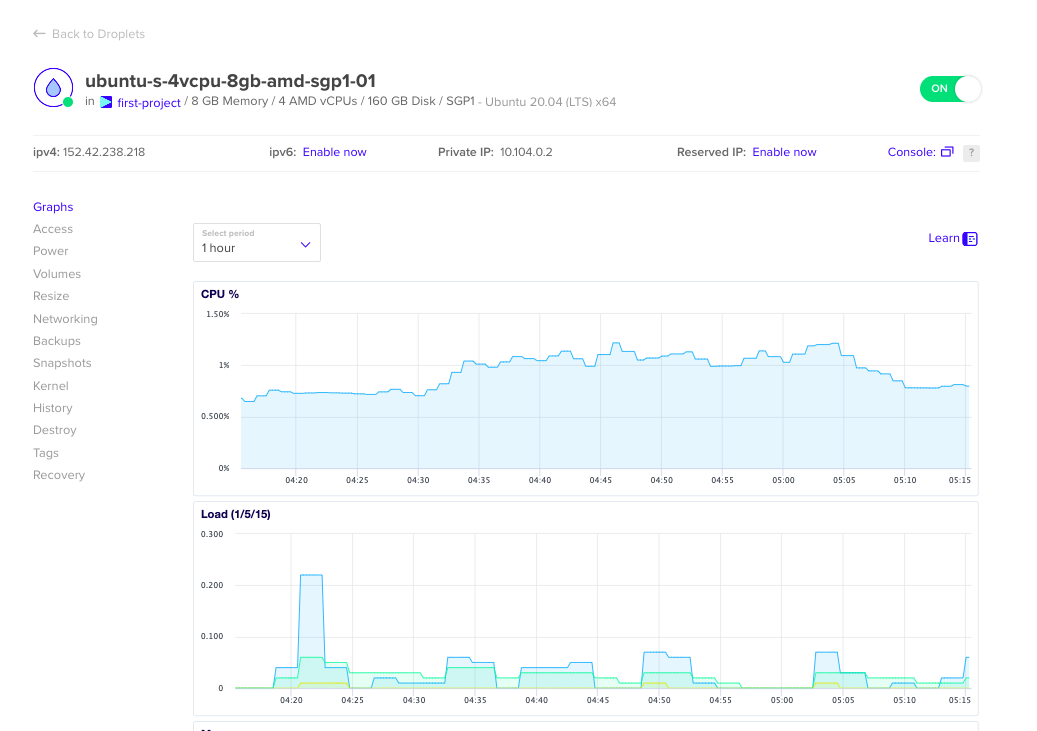
\includegraphics[width=1\textwidth]{figures/ch04/00-tampilan-digitalocean}
    \caption{Tampilan Dasbor VM DigitalOcean}
    \label{fig:00-tampilan-digitalocean}
\end{figure}


\section{Pemasangan dan Konfigurasi Perangkat Lunak}
Penelitian ini membandingkan kinerja Hadoop dan Spark pada \textit{platform cloud} DigitalOcean menggunakan alat pengujian data besar yang bernama HiBench pada lingkup \textit{Micro Benchmarks}, yaitu \textit{Word Count} dan \textit{Sort} dengan data masukan berupa teks yang dibuat oleh \textit{data generation} pada tahap persiapan. 

Sebelum memulai eksperimen, serangkaian pemeriksaan dilakukan untuk memastikan bahwa semua perangkat lunak yang terlibat berfungsi dengan baik. Tahapan ini penting untuk menjamin validitas hasil penelitian. Berikut adalah pemeriksaan yang dilakukan, yaitu
\begin{enumerate}
	\item \textbf{Pengecekan versi Hadoop}. Versi Hadoop yang digunakan dalam penelitian ini adalah 2.4.0. Verifikasi versi dilakukan melalui perintah \textit{hadoop version}, seperti yang ditunjukkan pada Gambar \ref{fig:versi-hadoop}. 
		\begin{figure}[h]
		    \centering
		    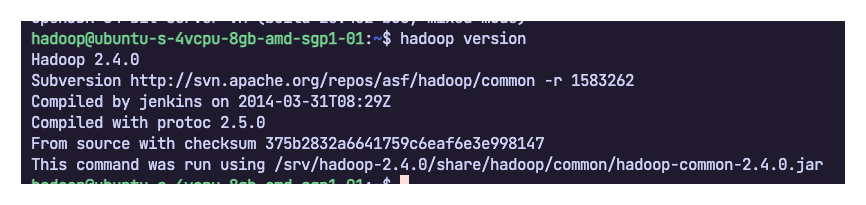
\includegraphics[width=0.8\textwidth]{figures/ch04/versi-hadoop}
		    \caption{Pengecekan Versi Hadoop}
		    \label{fig:versi-hadoop}
		\end{figure}
	\item \textbf{Pengecekan versi Spark}. Versi Spark yang digunakan adalah 2.1.3. Verifikasi dilakukan dengan perintah \textit{spark-submit --version}, seperti yang ditunjukkan pada Gambar \ref{fig:versi-spark}.
		\begin{figure}[h]
		    \centering
		    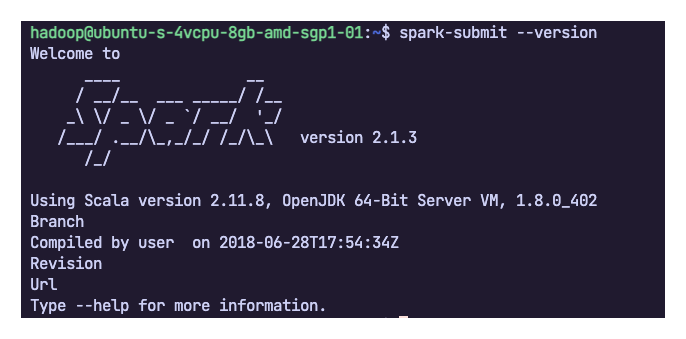
\includegraphics[width=0.8\textwidth]{figures/ch04/versi-spark}
		    \caption{Pengecekan Versi Spark}
		    \label{fig:versi-spark}
		\end{figure}
	\item \textbf{Pemeriksaan \textit{service} yang berjalan ketika tanpa beban kerja}. Status layanan (\textit{services}) yang berjalan pada komputer diperiksa dalam keadaan tanpa beban kerja (\textit{idle}). Layanan yang diharapkan aktif meliputi: Jps, ResourceManager, DataNode, NodeManager, NameNode, dan SecondaryNameNode. Gambar \ref{fig:service-dasar} menunjukkan hasil pemeriksaan layanan dasar.		
		\begin{figure}[h]
		    \centering
		    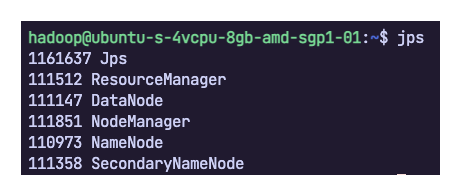
\includegraphics[width=0.8\textwidth]{figures/ch04/service-dasar}
		    \caption{Pengecekan \textit{Service} yang Berjalan (Normal)}
		    \label{fig:service-dasar}
		\end{figure}
	\newpage
	\item \textbf{Pemeriksaan \textit{service} yang berjalan ketika menggunakan Hadoop}. Ketika beban kerja Hadoop dijalankan, layanan tambahan seperti YarnChild, MRAppMaster, dan RunJar  diharapkan aktif, di samping layanan dasar yang telah disebutkan. Gambar \ref{fig:service-hadoop} menunjukkan hasil pemeriksaan layanan saat Hadoop aktif.
		\begin{figure}[h]
		    \centering
		    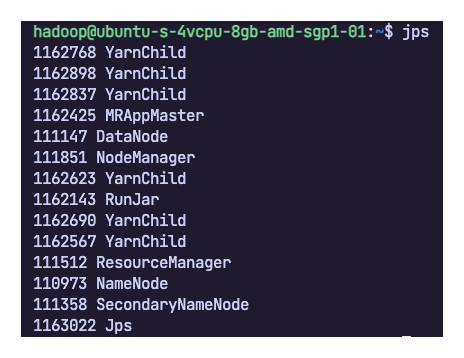
\includegraphics[width=0.7\textwidth]{figures/ch04/service-hadoop}
		    \caption{Pengecekan \textit{Service} yang Berjalan (Hadoop)}
		    \label{fig:service-hadoop}
		\end{figure}
	\item \textbf{Pemeriksaan \textit{service} yang berjalan ketika menggunakan Spark}. Ketika beban kerja Spark dijalankan, layanan seperti CoarseGrainedExecutorBackend, ExecutorLauncher, dan SparkSubmit diharapkan aktif, di samping layanan dasar.  Gambar \ref{fig:service-spark} menunjukkan hasil pemeriksaan layanan saat Spark aktif.
		\begin{figure}[h]
		    \centering
		    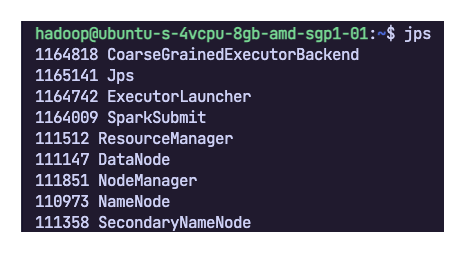
\includegraphics[width=0.8\textwidth]{figures/ch04/service-spark}
		    \caption{Pengecekan \textit{Service} yang Berjalan (Spark)}
		    \label{fig:service-spark}
		\end{figure}
\end{enumerate}

\newpage
\section{Eksperimen}
Selama pengujian, beberapa parameter pada HiBench, Hadoop, dan Spark dikonfigurasi secara tetap untuk menjaga konsistensi dan memungkinkan perbandingan yang adil. Tabel \ref{table:conf-hibench} dan Tabel \ref{table:conf-spark} merangkum konfigurasi parameter yang digunakan.

\begin{table}[h]
\caption{Konfigurasi HiBench}
\label{table:conf-hibench}
\scriptsize
\centering
\begin{tabular}{l c p{5cm}} 
\hline
%\multicolumn{1}{c}{\textbf{Nama Parameter}}  & \multicolumn{1}{c}{\textbf{Nilai}} & \multicolumn{1}{c}{\textbf{Keterangan}}  \\ \hline
\textbf{Nama Parameter} & \textbf{Nilai} & \textbf{Keterangan Parameter} \\ \hline
hibench.default.map.parallelism     & 8 & \textit{Mapper numbers} (Hadoop), \textit{partition numbers} (Spark)                          \\
hibench.default.shuffle.parallelism & 8 & \textit{Reducer numbers}  (Hadoop), \textit{shuffle partition} (Spark)\\ \hline                        
\end{tabular}
\end{table}

\begin{table}[h]
\caption{Konfigurasi Spark}
\label{table:conf-spark}
\scriptsize
\centering
\begin{tabular}{l c p{5cm}} 
\hline
\textbf{Nama Parameter} & \textbf{Nilai Parameter} & \textbf{Keterangan Parameter} \\ \hline
hibench.yarn.executor.num & 2 & Jumlah \textit{executor} \\
hibench.yarn.executor.cores & 4 & Jumlah \textit{core} CPU setiap \textit{executor}\\ 
spark.executor.memory & 4 GB & Jumlah memori setiap \textit{executor} \\
spark.driver.memory & 4 GB & Jumlah memori tiap \textit{driver} Spark\\ \hline                        
\end{tabular}
\end{table}

Parameter \textit{hibench.default.map.parallelism} memiliki peran yang berbeda pada Hadoop dan Spark. Pada Hadoop, parameter ini menentukan jumlah \textit{mapper}, yaitu proses yang bertanggung jawab untuk memproses data secara paralel pada tahap \textit{Map}. Pada Spark, parameter ini menentukan jumlah partisi data, yaitu unit pemrosesan dasar dalam Spark.

Parameter \textit{hibench.default.shuffle.parallelism} juga memiliki peran yang berbeda pada Hadoop dan Spark. Pada Hadoop, parameter ini menentukan jumlah \textit{Reducer}, yaitu proses yang bertanggung jawab untuk menggabungkan hasil dari tahap \textit{Map}. Pada Spark, parameter ini menentukan jumlah \textit{Shuffle partition}, yaitu jumlah partisi data yang digunakan selama tahap \textit{Shuffle}, yaitu proses pengocokan dan pengurutan data antara tahap \textit{Map} dan \textit{Reduce}.

%Berikut penjelasan mengenai parameter Spark pada Tabel \ref{table:conf-spark}:
%\begin{enumerate}
%	\item \textbf{hibench.yarn.executor.num}: Parameter ini menentukan jumlah \textit{executor} yang akan dialokasikan untuk aplikasi Spark. \textit{Executor} adalah proses yang berjalan pada node pekerja (\textit{worker node}) di kluster YARN dan bertanggung jawab untuk menjalankan task Spark.
%	\item \textbf{hibench.yarn.executor.cores}: Parameter ini menentukan jumlah core CPU yang dialokasikan untuk setiap \textit{executor}. Semakin banyak core yang dialokasikan, semakin banyak task yang dapat dijalankan secara paralel oleh setiap \textit{executor}.
%	\item \textbf{spark.executor.memory}: Parameter ini menentukan jumlah memori yang dialokasikan untuk setiap \textit{executor}. Memori ini digunakan untuk menyimpan data yang diproses oleh \textit{executor}, seperti RDD dan data yang di-\textit{cache}.
%	\item \textbf{spark.driver.memory}: Parameter ini menentukan jumlah memori yang dialokasikan untuk proses driver Spark. Driver bertanggung jawab untuk mengelola aplikasi Spark, menjadwalkan task, dan mengumpulkan hasil.
%\end{enumerate}

\section{Data Keluaran yang Dihasilkan}

Setiap pengujian akan menghasilkan berkas output berupa data HiBench \textit{Report} dan Dool \textit{System Monitoring}. Data HiBench \textit{Report} akan terlihat seperti pada Gambar \ref{fig:data-hibench-report}. Pada Gambar \ref{fig:data-hibench-report}, terlihat bahwa ekstensi berkasnya \textit{.report} dan terlihat beberapa data seperti jenis beban kerja, aplikasi yang digunakan, besar input data, durasi, dan \textit{throughput}.

\begin{figure}[h]
    \centering
    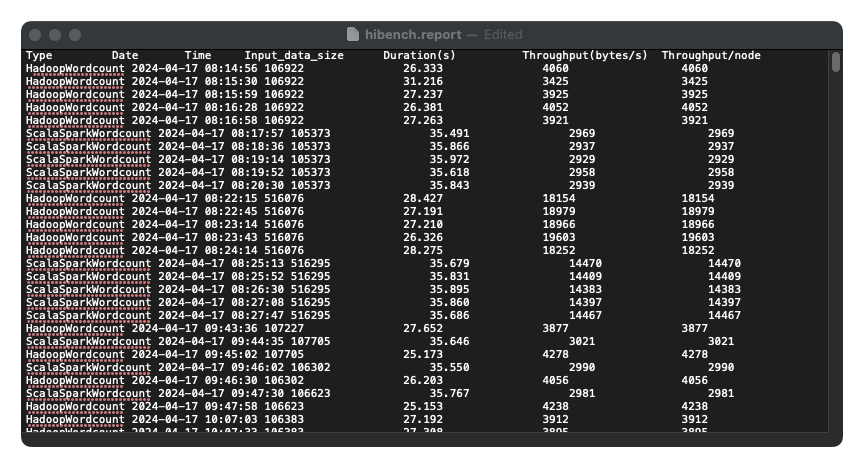
\includegraphics[width=0.9\textwidth]{figures/ch04/data-hibench}
    \caption{Data HiBench \textit{Report}}
    \label{fig:data-hibench-report}
\end{figure}

Dool, alat monitoring sistem, menghasilkan berkas CSV (\textit{comma-separated value}) untuk setiap perulangan eksperimen. Dengan demikian, terdapat sekitar 240 berkas CSV, seperti yang ditunjukkan pada Gambar \ref{fig:data-dool-luar}. Penamaan berkas mengikuti format: [jenis beban kerja]-[ukuran data]-[nomor perulangan]-[aplikasi]. Sebagai contoh, \textit{sort-fivegig-1-hadoop.csv} menunjukkan \textit{data monitoring} untuk beban kerja sort, data masukan 5 GB, perulangan pertama, dan aplikasi Hadoop.

\begin{figure}[h]
    \centering
    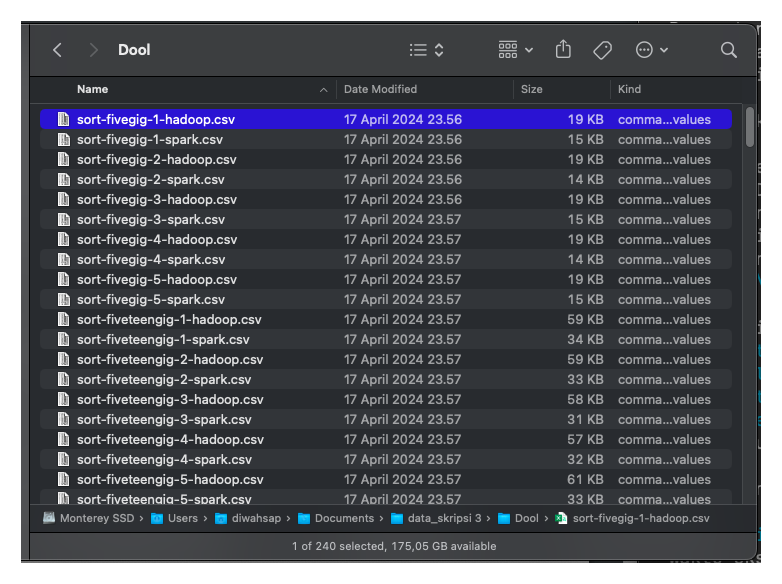
\includegraphics[width=0.75\textwidth]{figures/ch04/data-dool-luar}
    \caption{Berkas Dool}
    \label{fig:data-dool-luar}
\end{figure}

Struktur data Dool, yang ditunjukkan pada Gambar \ref{fig:data-dool-dalam}, mencakup baris \textit{header} (baris 1-4) dan nama kolom (baris 6). Data ini akan dianalisis lebih lanjut untuk mendapatkan \textit{insight} tentang kinerja Hadoop dan Spark.

\begin{landscape}
\begin{figure}[h]
    \centering
    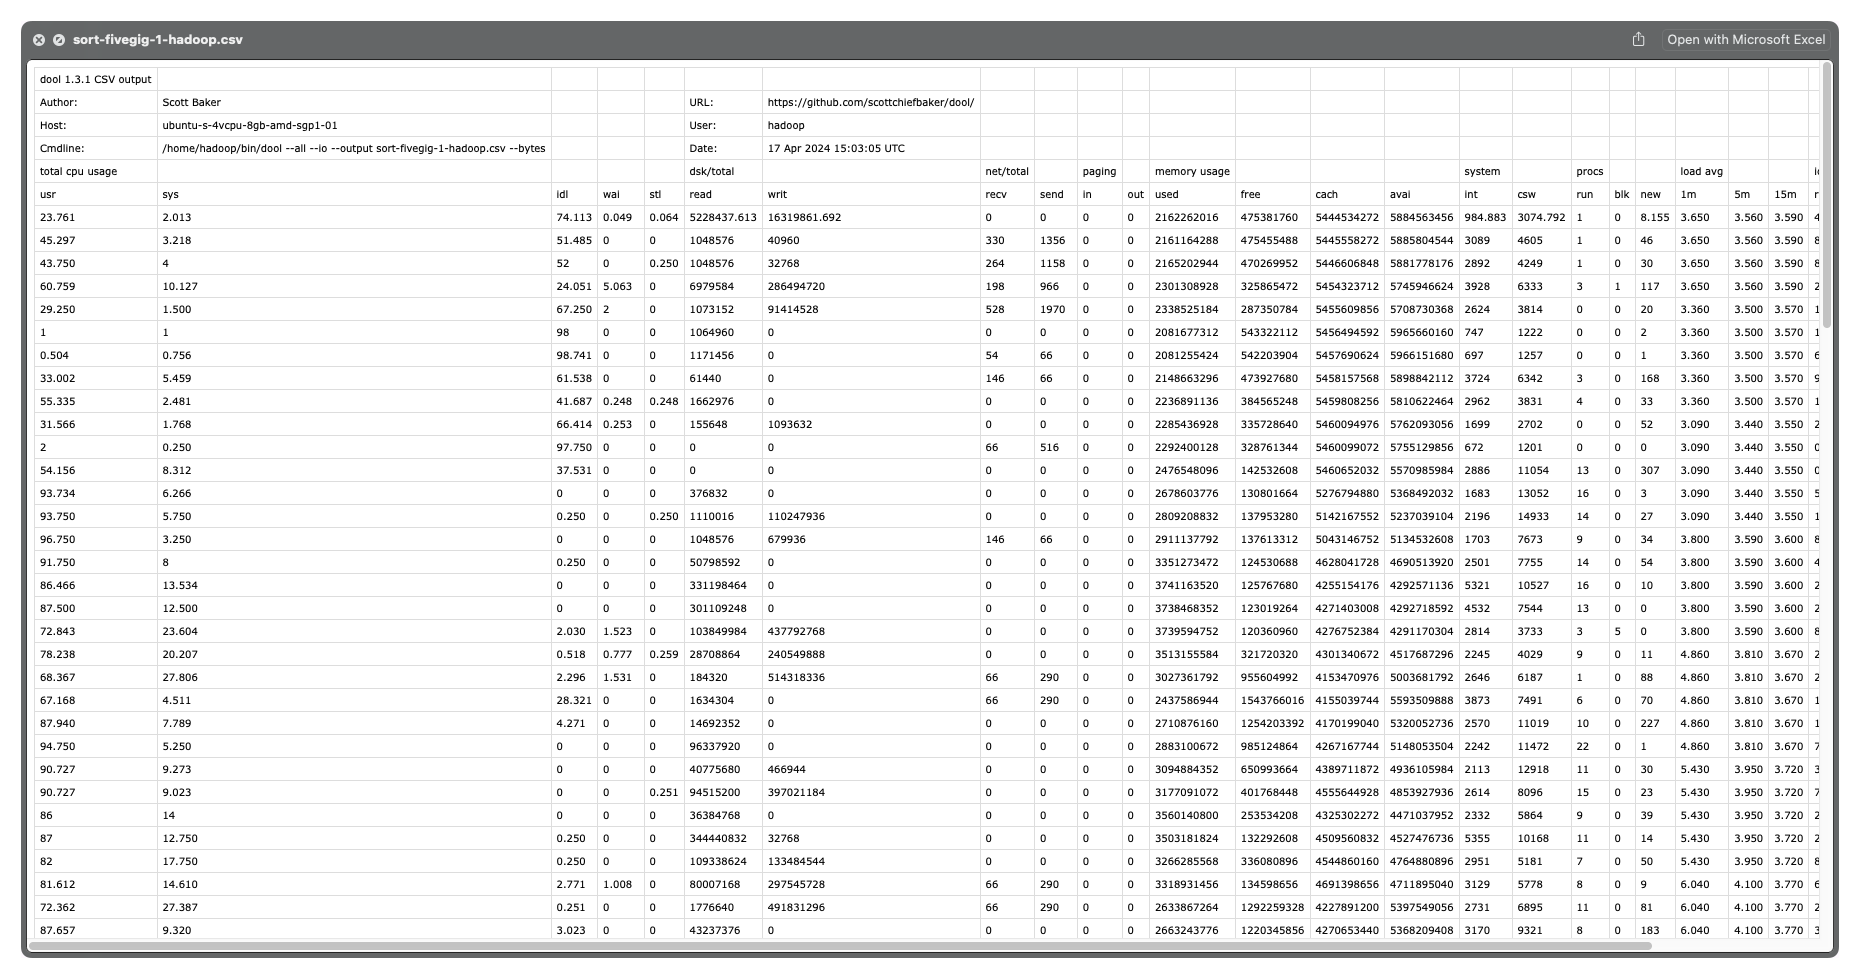
\includegraphics[width=\linewidth, height=0.5\linewidth]{figures/ch04/data-dool-dalam}
    \caption{Contoh Data Dool}
    \label{fig:data-dool-dalam}
\end{figure}
\end{landscape}

\newpage
\section {Analisis dan Evaluasi Hasil Eksperimen: Kinerja}
\subsection{Persebaran Waktu Eksekusi pada Hadoop dan Spark}
Waktu eksekusi adalah durasi yang diperlukan untuk memproses data. Nilai parameter ini diperoleh dengan menghitung selisih antara waktu awal dan waktu akhir saat Apache Hadoop dan Apache Spark dijalankan atau dihentikan untuk memproses input data dengan beban kerja masing-masing. Satuan pengukuran untuk parameter waktu eksekusi adalah detik. Setiap beban kerja dilakukan sebanyak lima kali pengulangan untuk mendapatkan hasil yang lebih akurat dan representatif.

Gambar \ref{fig:lama-waktu-eksekusi-sort} dan Gambar \ref{fig:lama-waktu-eksekusi-wordcount} menyajikan \textit{scatter plot} yang membandingkan performa Hadoop dan Spark dalam dua tugas pemrosesan data yang berbeda, yaitu \textit{sort} dan \textit{word count}. Sumbu x pada kedua gambar menunjukkan variasi ukuran input data, mulai dari 100 KB hingga 15 GB, sementara sumbu y menunjukkan waktu eksekusi dalam detik.

\begin{figure}[h]
    \centering
    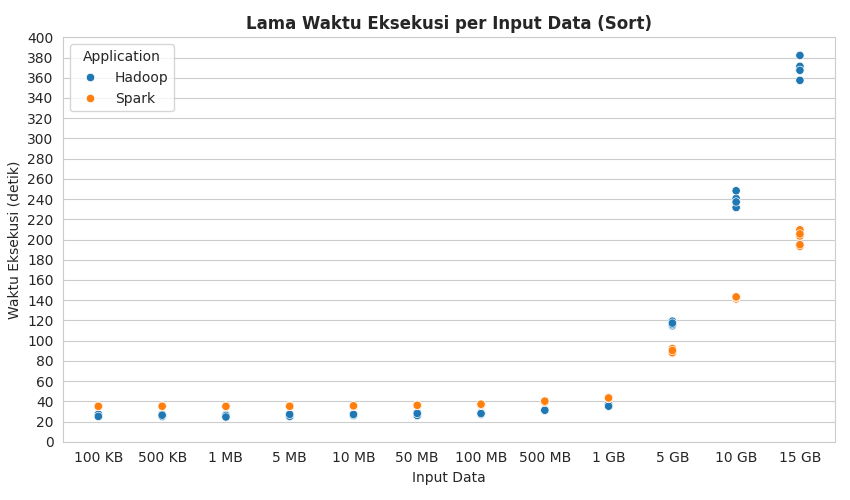
\includegraphics[width=1\textwidth]{figures/ch04/1-lama-waktu-eksekusi-sort.png}
    \caption{Persebaran Waktu Eksekusi \textit{Sort} (Hadoop, Spark)}
    \label{fig:lama-waktu-eksekusi-sort}
\end{figure}

Pada Gambar \ref{fig:lama-waktu-eksekusi-sort}, terlihat bahwa waktu eksekusi Hadoop untuk input data 100 KB hingga 1 GB secara konsisten lebih cepat dibandingkan Spark. Hadoop berada pada rentang waktu 20-40 detik, sedangkan Spark berada pada rentang waktu 35-45 detik.

Namun, untuk input data sebesar 5 GB, Spark menunjukkan waktu eksekusi yang lebih cepat dibandingkan Hadoop. Spark berada pada rentang 80-100 detik, sementara Hadoop berada pada rentang 110-125 detik. Perbedaan performa ini semakin signifikan seiring bertambahnya ukuran data, terutama pada ukuran data 10 GB dan 15 GB. Perbedaan waktu eksekusi antara Hadoop dan Spark semakin jauh pada beban kerja \textit{sort} dengan ukuran data yang lebih besar.

Tabel \ref{table:4-sort-dur-table} menunjukkan data yang lebih rinci mengenai durasi waktu eksekusi \textit{sort} untuk Hadoop dan Spark. Berdasarkan tabel tersebut, terlihat bahwa untuk ukuran input data yang kecil hingga menengah, Hadoop relatif lebih cepat daripada Spark. Namun, seiring bertambahnya ukuran input data, Spark menunjukkan performa yang lebih baik dengan waktu eksekusi yang lebih singkat.

Perbedaan kinerja ini dapat dilihat dari kolom "Waktu Eksekusi (maks)" dan "Waktu Eksekusi (min)". Misalnya, untuk input data 100 KB, Hadoop memiliki waktu eksekusi maksimum 27.275 detik, sedangkan Spark memiliki waktu eksekusi maksimum 35.534 detik. Hal ini menunjukkan bahwa Hadoop lebih stabil dengan waktu eksekusi yang lebih konsisten, namun secara rata-rata Spark lebih cepat. Namun, ketika input data mencapai 10 GB, waktu eksekusi maksimum Hadoop mencapai 248.255 detik, sementara Spark hanya mencapai 143.217 detik. Perbedaan yang signifikan ini menunjukkan bahwa Spark mampu menangani input data yang besar dengan lebih efisien dibandingkan Hadoop. Hal ini juga dapat dilihat dari kolom "Standar Deviasi" yang menunjukkan bahwa waktu eksekusi Spark lebih stabil daripada Hadoop untuk ukuran input data yang besar.

\begin{table}[h]
  \centering
  \caption{Statistika Deskriptif Lama Waktu Eksekusi (\textit{Sort})}
  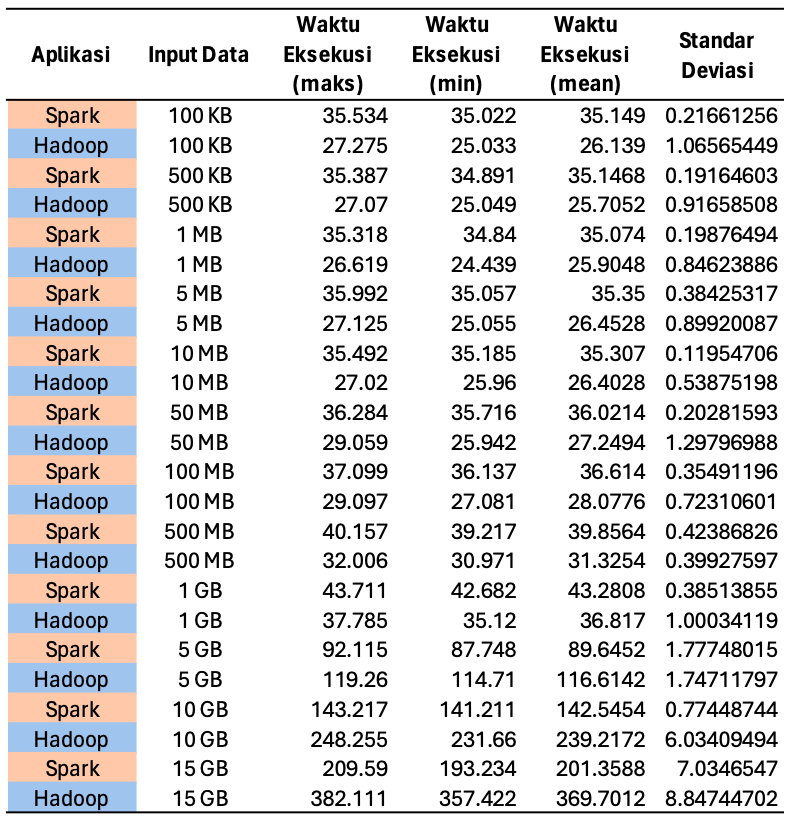
\includegraphics[width=0.75\textwidth]{figures/ch04/4-sort-dur-table}
  \label{table:4-sort-dur-table}
\end{table}

\begin{figure}[h]
    \centering
    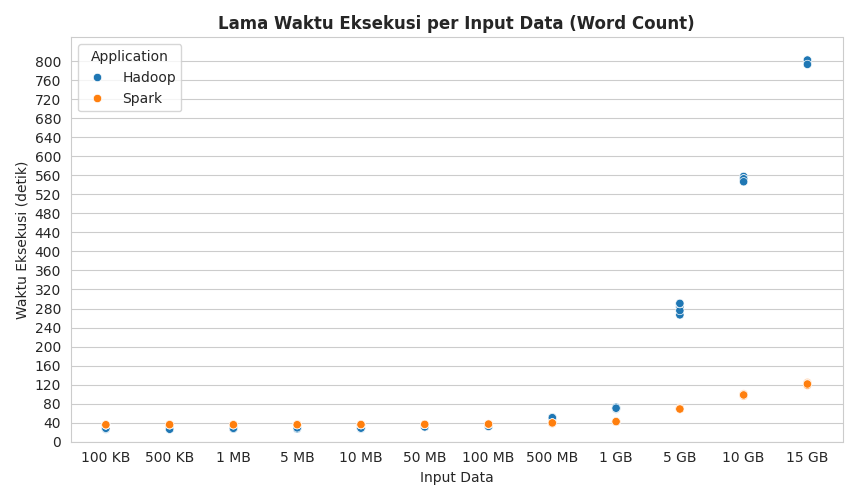
\includegraphics[width=1\textwidth]{figures/ch04/1-lama-waktu-eksekusi-wordcount.png}
    \caption{Persebaran Waktu Eksekusi \textit{Word Count} (Hadoop, Spark)}
    \label{fig:lama-waktu-eksekusi-wordcount}
\end{figure}

\newpage
Pada Gambar \ref{fig:lama-waktu-eksekusi-wordcount}, Spark menunjukkan performa yang lebih baik dibandingkan Hadoop untuk ukuran input data 500 MB, 1 GB, 5 GB, 10 GB, dan 15 GB pada beban kerja \textit{word count}. Namun, untuk ukuran input data 100 KB hingga 100 MB, Hadoop masih lebih unggul. Waktu eksekusi Hadoop untuk input data 100 KB hingga 100 MB berada pada rentang 20-40 detik, meskipun perbedaannya tidak signifikan dibandingkan Spark karena titik data Hadoop dan Spark saling berdekatan.

\begin{table}[h]
  \centering
  \caption{Statistika Deskriptif Lama Waktu Eksekusi (\textit{Word Count})}
  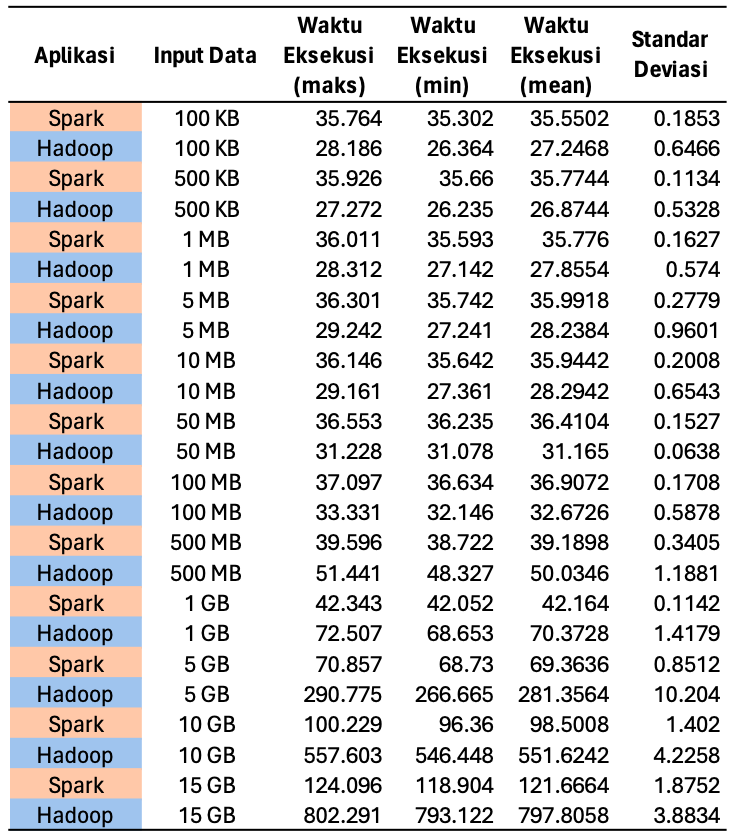
\includegraphics[width=0.75\textwidth]{figures/ch04/4-wc-dur-table}
  \label{table:4-wc-dur-table}
\end{table}

Tabel \ref{table:4-wc-dur-table} menunjukkan data yang lebih rinci mengenai durasi waktu eksekusi \textit{word count} untuk Hadoop dan Spark. Berdasarkan tabel tersebut, terlihat bahwa Hadoop lebih cepat daripada Spark untuk ukuran input data yang kecil hingga menengah yaitu pada 100 KB-100 MB, tetapi Spark lebih cepat untuk ukuran input data yang besar.

Perbedaan kinerja ini dapat dilihat dari kolom "Waktu Eksekusi (maks)" dan "Waktu Eksekusi (min)". Misalnya, untuk input data 100 KB, Hadoop memiliki waktu eksekusi maksimum 28.186 detik, sedangkan Spark memiliki waktu eksekusi maksimum 35.764 detik. Hal ini menunjukkan bahwa Hadoop lebih stabil dengan waktu eksekusi yang lebih konsisten, namun secara rata-rata Spark lebih cepat. Namun, ketika input data mencapai 10 GB, waktu eksekusi maksimum Hadoop mencapai 557.603 detik, sementara Spark hanya mencapai 100.229 detik. Perbedaan yang signifikan ini menunjukkan bahwa Spark mampu menangani input data yang besar dengan lebih efisien dibandingkan Hadoop. Hal ini juga dapat dilihat dari kolom "Standar Deviasi" yang menunjukkan bahwa waktu eksekusi Spark lebih stabil daripada Hadoop untuk ukuran input data yang besar.

Hasil ini menunjukkan bahwa Spark lebih unggul dan konsisten dibandingkan Hadoop dalam menangani tugas pemrosesan data yang lebih besar, dengan rincian sebagai berikut:
\begin{enumerate}
\item Untuk beban kerja \textit{sort}, Spark lebih unggul mulai dari ukuran input data 5 GB, 10 GB, dan 15 GB.
\item Untuk beban kerja \textit{word count}, Spark lebih unggul mulai dari ukuran input data 500 MB, 1 GB, 5 GB, 10 GB, dan 15 GB.
\end{enumerate}

Secara keseluruhan, Spark menunjukkan kinerja yang lebih baik dalam menangani data berukuran besar, sementara Hadoop lebih efisien untuk data berukuran kecil hingga menengah.

% ----------------------------------------
\subsection {Persebaran \textit{Throughput} pada Hadoop dan Spark}

\textit{Throughput} adalah kecepatan pertukaran data per detik. Kegiatan pertukaran data tersebut terjadi pada \textit{node} yang dipakai dalam komputer komputasi, saat Hadoop maupun Spark memproses data. Oleh karena itu, semakin tinggi nilai \textit{throughput}, semakin sedikit waktu yang dibutuhkan untuk menyelesaikan komputasi. Satuan \textit{throughput} pada penelitian ini adalah MB/s (mega bita per detik).

Gambar di bawah akan menyajikan \textit{scatter plot} yang membandingkan \textit{throughput} Hadoop dan Spark dalam dua tugas pemrosesan data, yaitu \textit{sort} (Gambar \ref{fig:throughput-sort}) dan \textit{word count} (Gambar \ref{fig:throughput-wordcount}). Sumbu x pada kedua gambar menunjukkan variasi ukuran input data, sedangkan sumbu y menunjukkan \textit{throughput} dalam MB/s.

\begin{figure}[h]
    \centering
    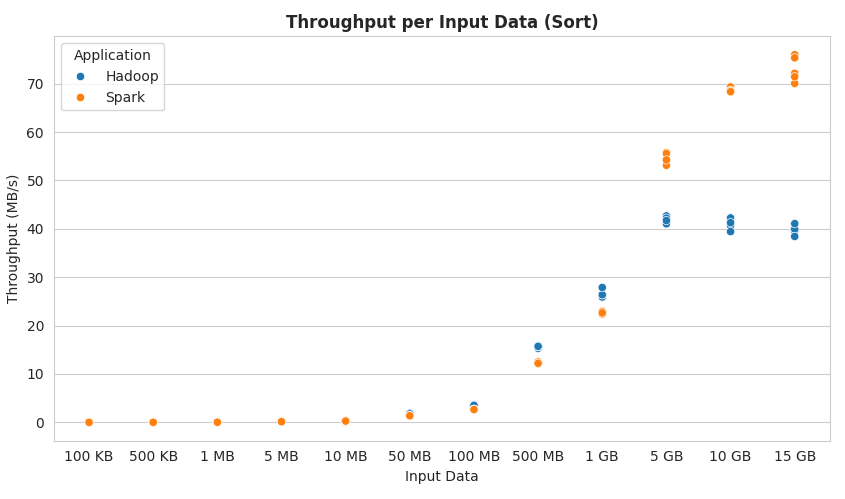
\includegraphics[width=1\textwidth]{figures/ch04/1-throughput-sort.png}
    \caption{\textit{Throughput Sort} (Hadoop, Spark)}
    \label{fig:throughput-sort}
\end{figure}

Pada tugas \textit{sort} (Gambar \ref{fig:throughput-sort}), Spark menunjukkan peningkatan \textit{throughput} yang signifikan seiring dengan bertambahnya ukuran data. Pada ukuran data terbesar (15 GB), Spark mencapai \textit{throughput} sekitar 70 MB/s. Sebaliknya, Hadoop menunjukkan peningkatan \textit{throughput} yang lebih lambat dan hanya mencapai sekitar 40 MB/s pada ukuran data yang sama. Hal ini menunjukkan bahwa Spark mampu melakukan pertukaran data yang lebih besar daripada Hadoop.

\begin{table}[h]
  \centering
  \caption{Statistika Deskriptif \textit{Throughput} (\textit{Sort})}
  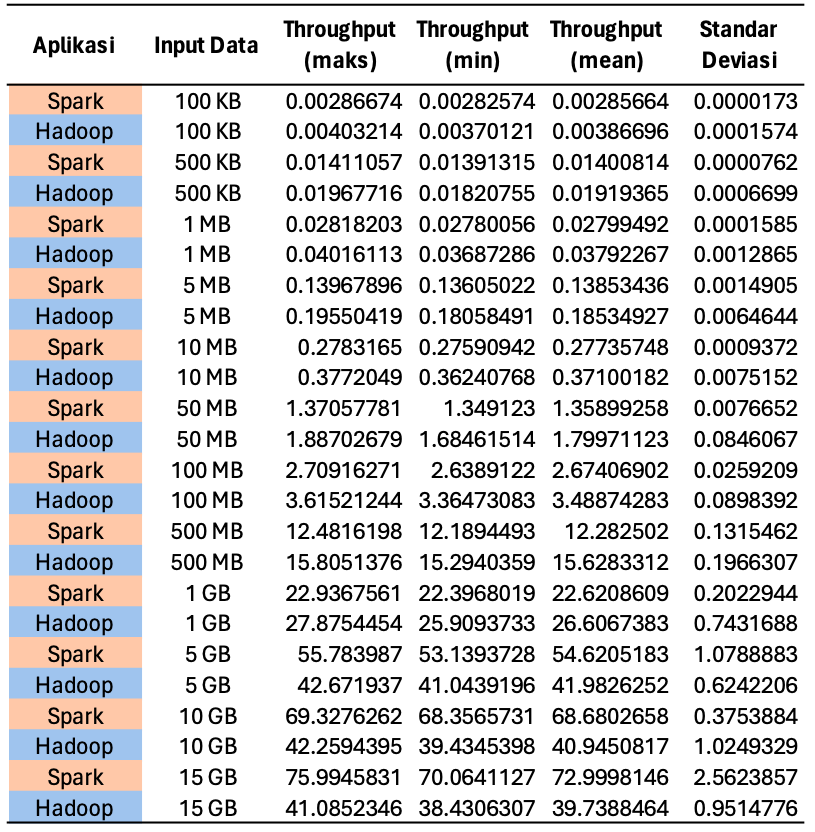
\includegraphics[width=0.75\textwidth]{figures/ch04/4-sort-th-table}
  \label{table:4-sort-th-table}
\end{table}

Tabel \ref{table:4-sort-th-table} menunjukkan data yang lebih rinci mengenai \textit{throughput} \textit{sort} untuk Hadoop dan Spark. Berdasarkan tabel tersebut, terlihat bahwa Hadoop memiliki \textit{throughput} yang lebih rendah dibandingkan Spark, terutama pada ukuran data yang lebih besar.
Perbedaan kinerja ini dapat dilihat dari kolom "Throughput (maks)" dan "Throughput (min)". Misalnya, untuk input data 100 KB, Hadoop memiliki \textit{throughput} maksimum 0.00403214 MB/s, sedangkan Spark memiliki \textit{throughput} maksimum 0.00286674 MB/s. Hal ini menunjukkan bahwa Hadoop lebih stabil dengan \textit{throughput} yang lebih konsisten, namun secara rata-rata Spark lebih cepat. Namun, ketika input data mencapai 10 GB, \textit{throughput} maksimum Hadoop mencapai 42.2594395 MB/s, sementara Spark mencapai 69.3276262 MB/s. Perbedaan yang signifikan ini menunjukkan bahwa Spark mampu menangani input data yang besar dengan lebih efisien dibandingkan Hadoop. Hal ini juga dapat dilihat dari kolom "Standar Deviasi" yang menunjukkan bahwa \textit{throughput} Spark lebih stabil daripada Hadoop untuk ukuran input data yang besar.

\begin{figure}[h]
    \centering
    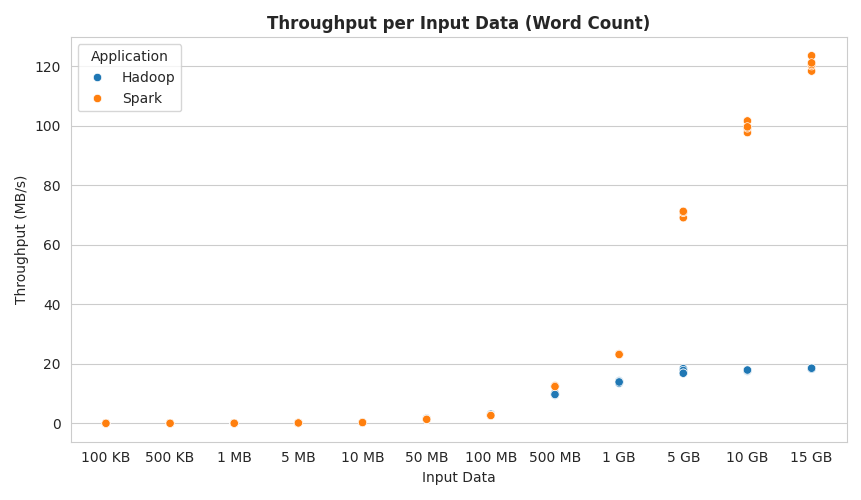
\includegraphics[width=1\textwidth]{figures/ch04/1-throughput-wordcount.png}
    \caption{\textit{Throughput Word Count} (Hadoop, Spark)}
    \label{fig:throughput-wordcount}
\end{figure}

Pada beban kerja \textit{word count} (Gambar \ref{fig:throughput-wordcount}), Spark mencapai \textit{throughput} yang lebih tinggi daripada Hadoop. Perbedaan \textit{throughput} paling mencolok terlihat pada ukuran data terbesar (15 GB), di mana Spark mencapai \textit{throughput} lebih dari 120 MB/s, sedangkan Hadoop hanya mencapai sekitar 20 MB/s. Meskipun Spark menunjukkan peningkatan \textit{throughput} yang signifikan pada ukuran data besar (1 GB, 5 GB, 10 GB, dan 15 GB), pada data input yang lebih kecil, 100 KB sampai 100 MB, perbedaan \textit{throughput} antara Hadoop dan Spark tidak berbeda jauh untuk \textit{word count}.

\begin{table}[h]
  \centering
  \caption{Statistika Deskriptif \textit{Throughput} (\textit{Word Count})}
  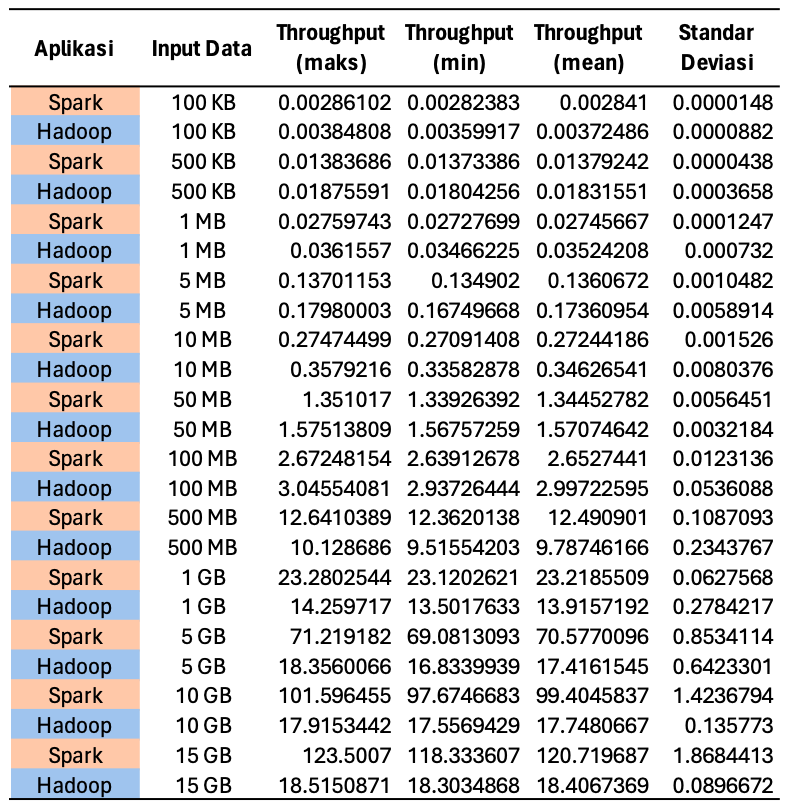
\includegraphics[width=0.75\textwidth]{figures/ch04/4-wc-th-table}
  \label{table:4-wc-th-table}
\end{table}

Tabel \ref{table:4-wc-th-table} menunjukkan data yang lebih rinci mengenai \textit{throughput} \textit{word count} untuk Hadoop dan Spark. Berdasarkan tabel tersebut, terlihat bahwa Hadoop memiliki \textit{throughput} yang lebih rendah dibandingkan Spark, terutama pada ukuran data yang lebih besar.
Perbedaan kinerja ini dapat dilihat dari kolom "Throughput (maks)" dan "Throughput (min)". Misalnya, untuk input data 100 KB, Hadoop memiliki \textit{throughput} maksimum 0.00384808 MB/s, sedangkan Spark memiliki \textit{throughput} maksimum 0.00286102 MB/s. Hal ini menunjukkan bahwa Hadoop lebih stabil dengan \textit{throughput} yang lebih konsisten, namun secara rata-rata Spark lebih cepat. Namun, ketika input data mencapai 10 GB, \textit{throughput} maksimum Hadoop mencapai 17.9153442 MB/s, sementara Spark mencapai 101.596455 MB/s.

Hasil ini menunjukkan bahwa Spark lebih unggul dalam menangani data berukuran besar untuk kedua tugas pemrosesan data tersebut. Spark mampu mempertahankan \textit{throughput} yang lebih tinggi dibandingkan Hadoop, terutama saat menangani data berukuran besar, dengan rincian sebagai berikut:
\begin{enumerate}
\item Untuk beban kerja \textit{sort}, Spark lebih unggul pada ukuran data 1 GB, 5 GB, 10 GB, dan 15 GB.
\item Untuk beban kerja \textit{word count}, Spark lebih unggul pada ukuran data 1 GB, 5 GB, 10 GB, dan 15 GB.
\end{enumerate}

Secara keseluruhan, Spark menunjukkan kinerja yang lebih baik dalam hal \textit{throughput} terutama pada data berukuran besar, sementara Hadoop masih menunjukkan performa yang kompetitif pada data berukuran kecil hingga menengah.

% ----------------------------------------

%\subsection {Rata-rata Waktu Eksekusi pada Hadoop dan Spark}
%
%Gambar \ref{fig:mean-dur-sort} dan Gambar \ref{fig:mean-dur-wordcount} menyajikan \textit{line plot} yang menggambarkan rata-rata waktu eksekusi Hadoop dan Spark untuk tugas \textit{sort} dan \textit{word count} dengan berbagai ukuran data. Sumbu x pada kedua gambar menunjukkan ukuran input data, sedangkan sumbu y menunjukkan rata-rata waktu eksekusi dalam detik. Garis vertikal pada kedua gambar menunjukkan titik di mana Spark mulai menunjukkan performa yang lebih cepat dibandingkan Hadoop.
%
%\begin{figure}[h]
%    \centering
%    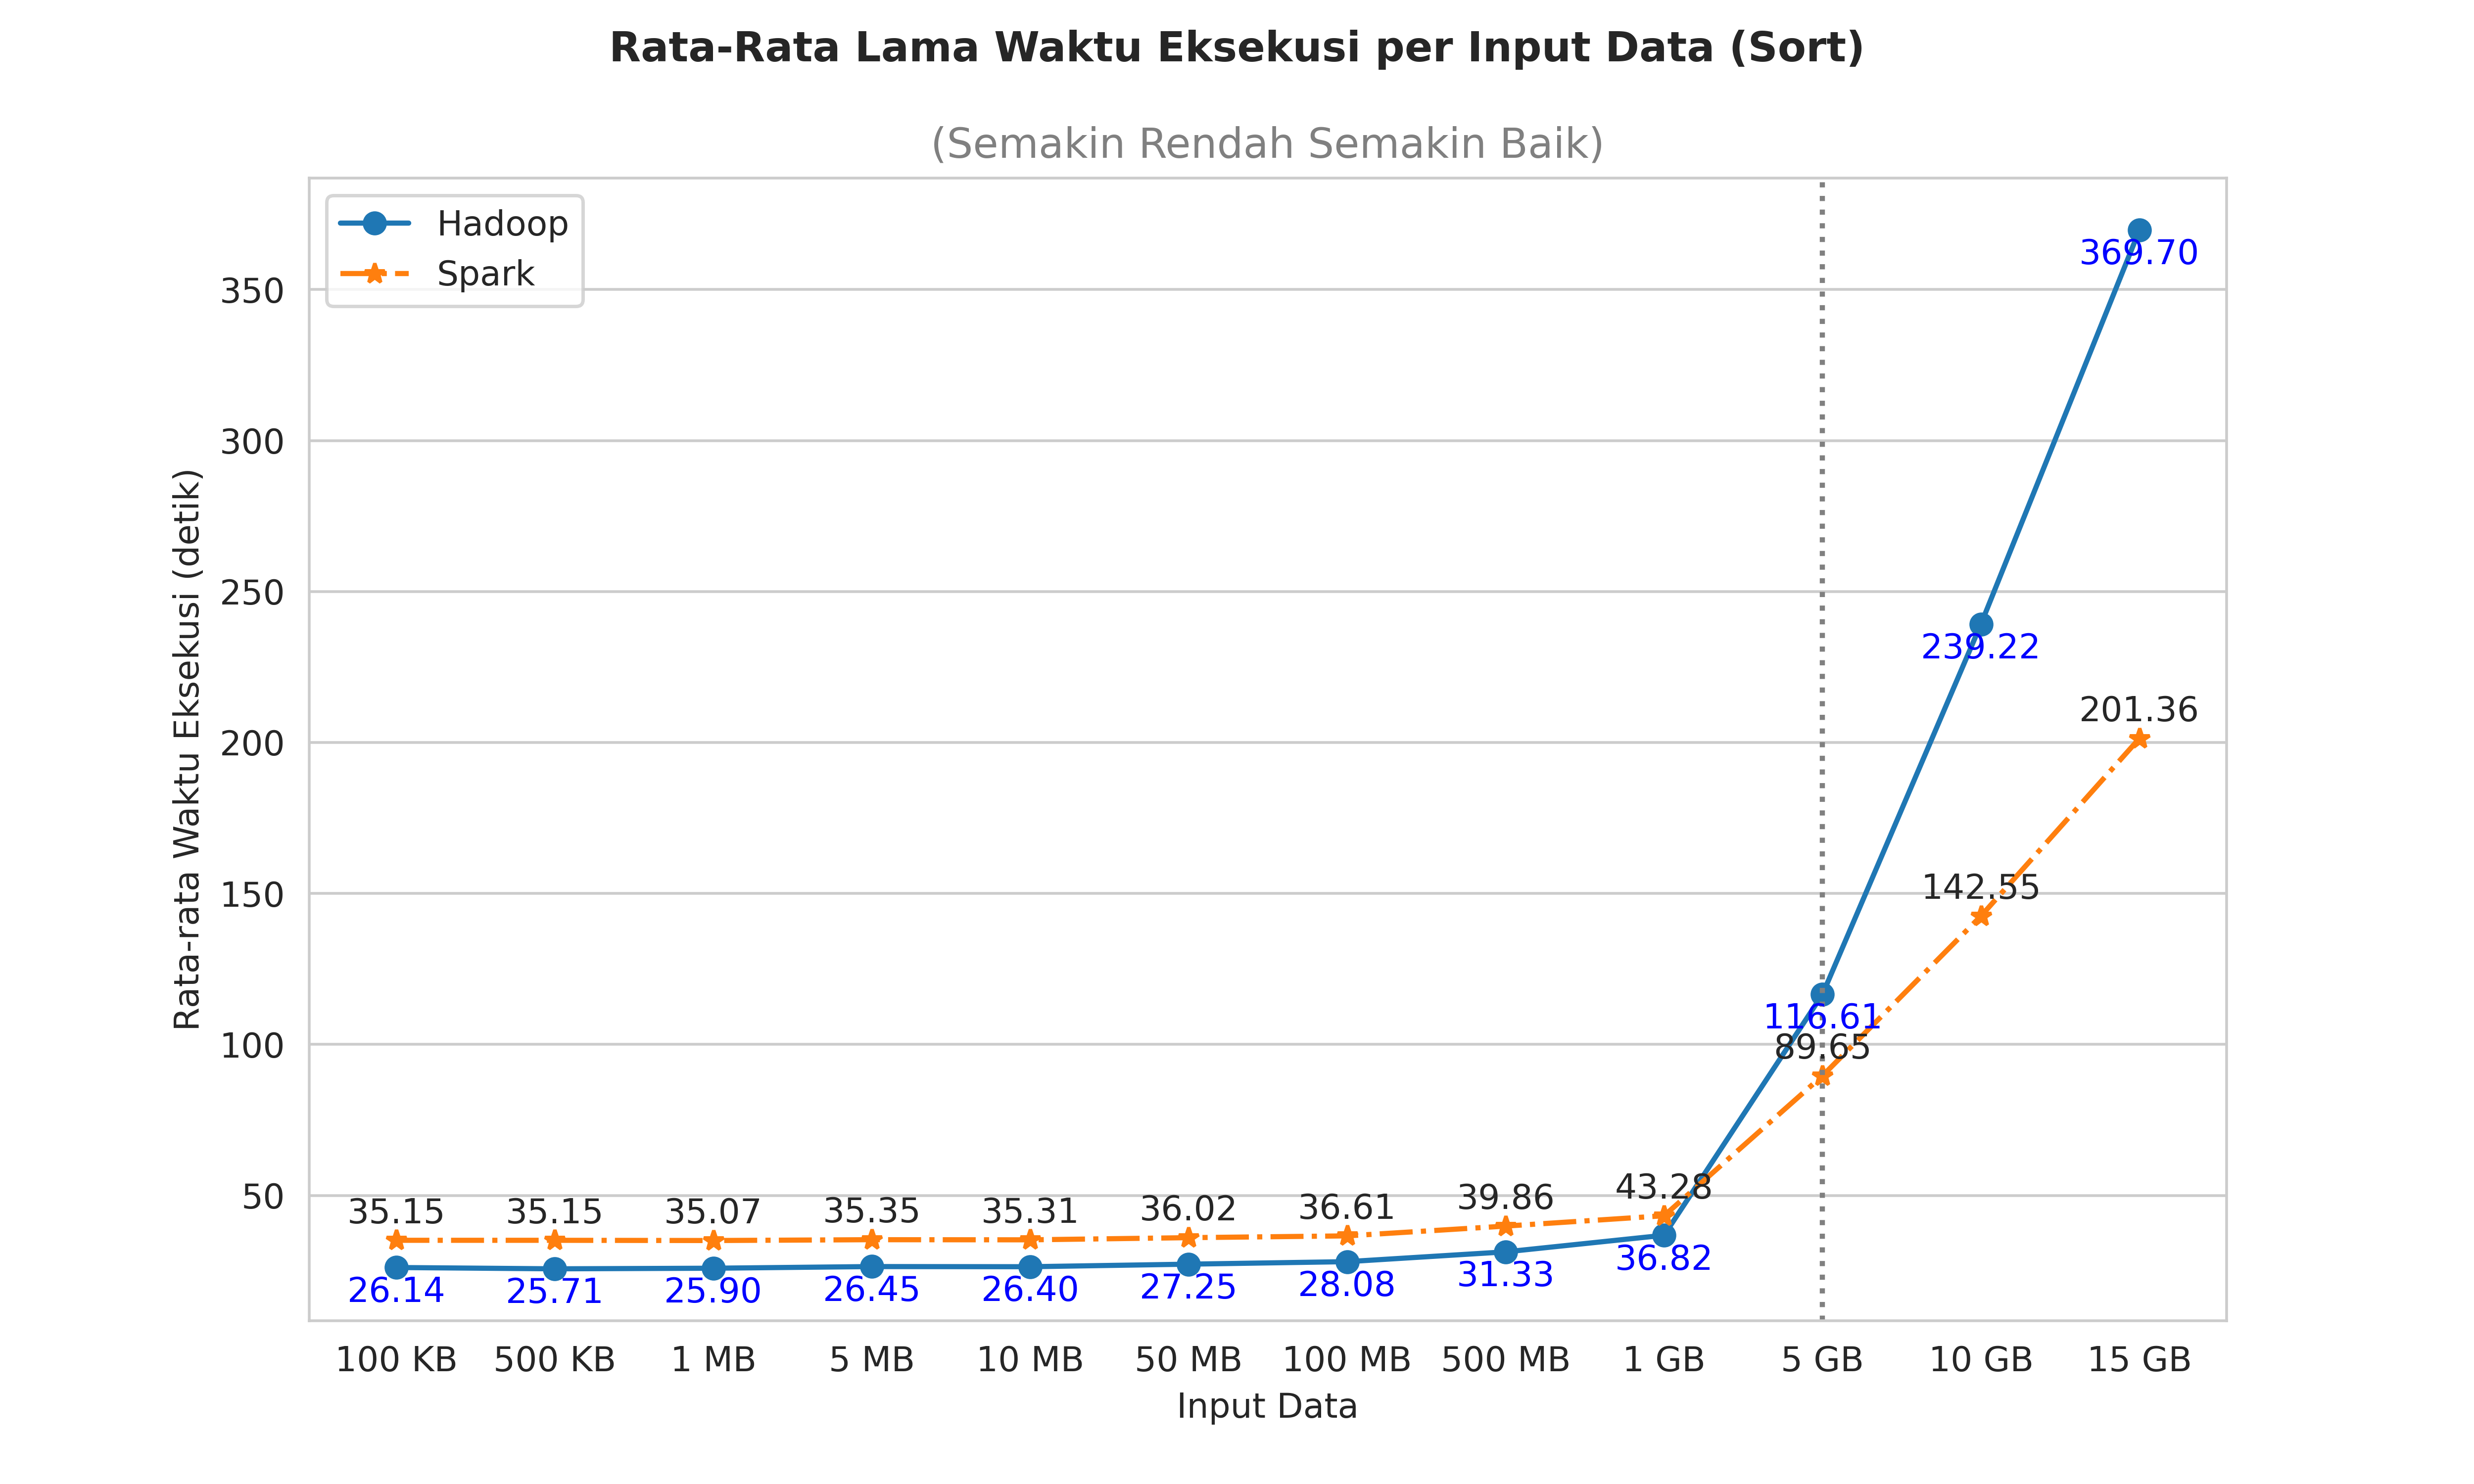
\includegraphics[width=1\textwidth]{figures/ch04/2-mean-lama-waktu-eksekusi-sort.png}
%    \caption{Rata-rata Waktu Eksekusi \textit{(Sort)}}
%    \label{fig:mean-dur-sort}
%\end{figure}
%
%Pada Gambar \ref{fig:mean-dur-sort}, terlihat bahwa Hadoop secara konsisten memiliki waktu eksekusi yang lebih rendah daripada Spark untuk ukuran input data 100 KB-1 GB pada tugas \textit{sort}. Perbedaan performa mulai terlihat pada input data 5 GB, di mana waktu eksekusi pada Hadoop mulai meningkat secara eksponensial, sementara Spark menunjukkan kenaikan yang lebih moderat. Pada ukuran data terbesar (15 GB), waktu eksekusi Hadoop mencapai sekitar 369,70 detik, sedangkan Spark hanya mencapai sekitar 201,36 detik.
%
%\begin{figure}[h]
%    \centering
%    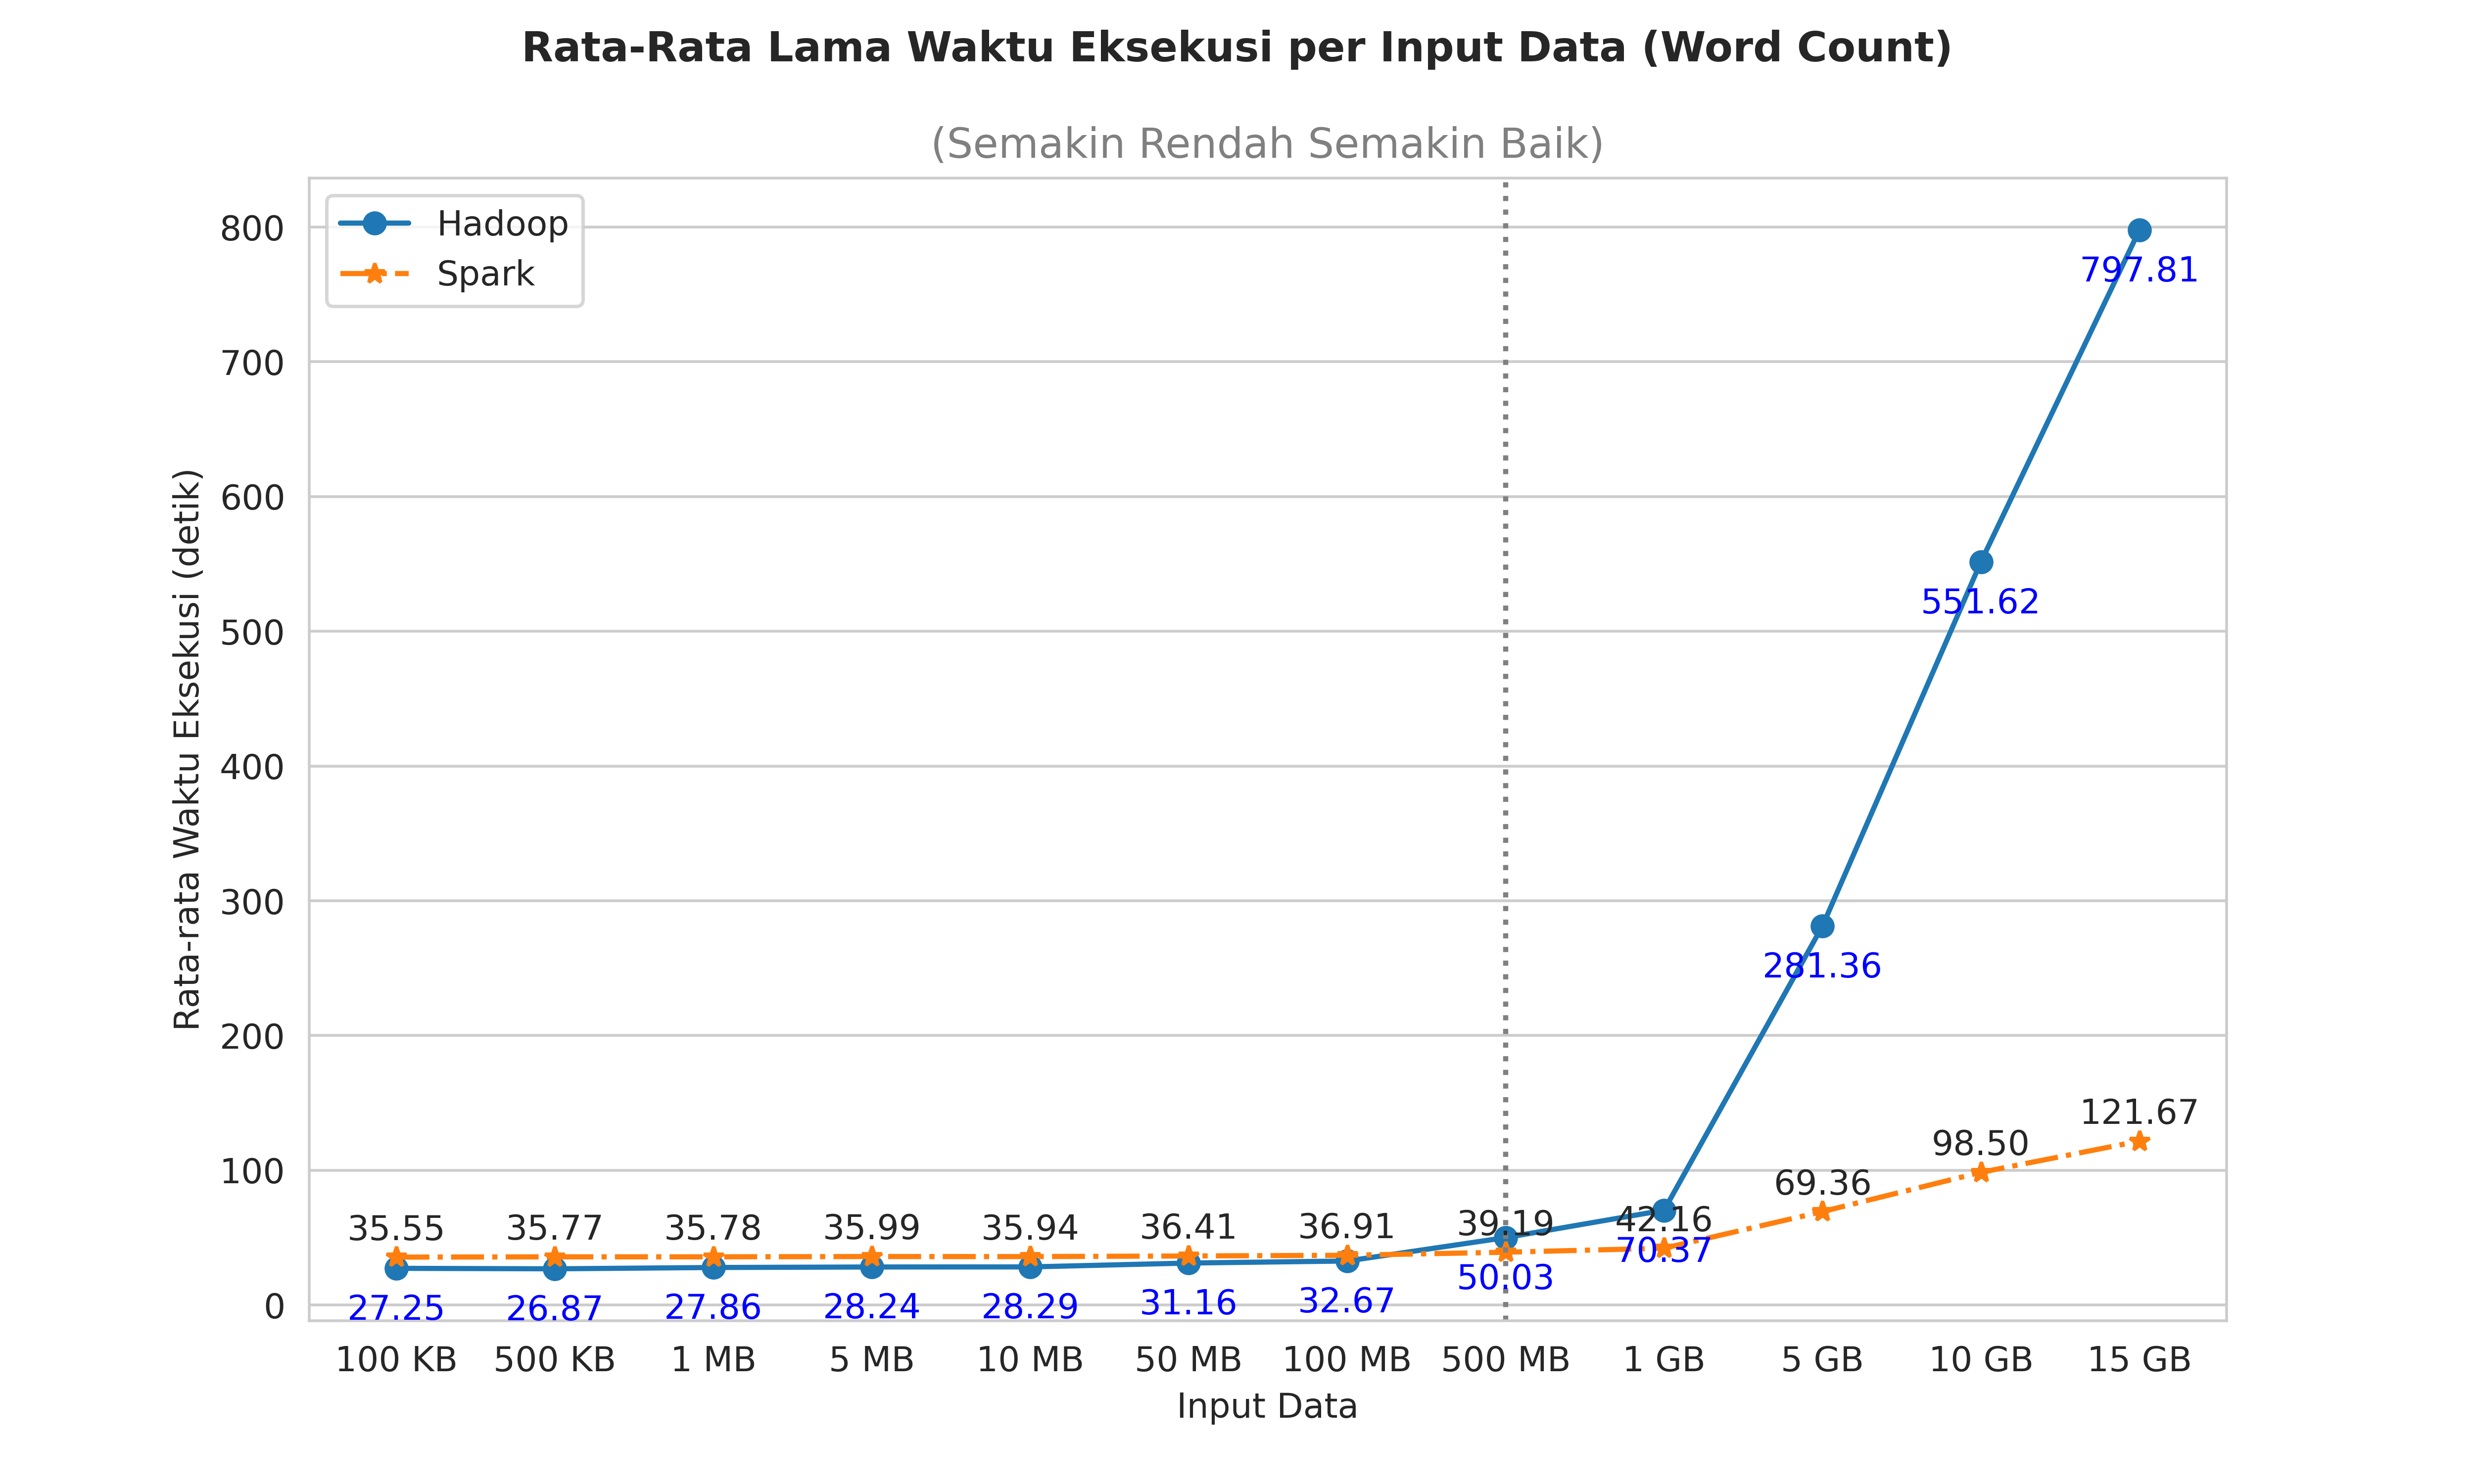
\includegraphics[width=1\textwidth]{figures/ch04/2-mean-lama-waktu-eksekusi-wordcount.png}
%    \caption{Rata-rata Waktu Eksekusi \textit{(Word Count)}}
%    \label{fig:mean-dur-wordcount}
%\end{figure}
%
%Pada Gambar \ref{fig:mean-dur-wordcount}, Spark juga menunjukkan performa yang lebih baik daripada Hadoop pada sebagian besar ukuran data pada tugas \textit{word count}, khususnya mulai dari input data 500 MB sampai 15 GB. Lama waktu eksekusi beban kerja pada Hadoop mulai mengalami kenaikan sejak input data 500 MB. Sedangkan, Spark baru mengalami kenaikan waktu eksekusi pada input data 5 GB. Pada ukuran data terbesar (15 GB), waktu eksekusi Hadoop mencapai sekitar 797,81 detik, sedangkan Spark hanya mencapai sekitar 121,67 detik.
%
%Hasil ini menunjukkan bahwa Spark lebih unggul dalam menangani data berukuran besar untuk kedua tugas pemrosesan data tersebut. Spark mampu mempertahankan waktu eksekusi yang lebih rendah dibandingkan Hadoop, terutama saat menangani data berukuran besar, dengan rincian sebagai berikut:
%\begin{enumerate}
%\item Untuk beban kerja \textit{sort}, Hadoop lebih unggul pada ukuran data 100 KB hingga 1 GB, sedangkan Spark mulai unggul pada ukuran data 5 GB dan seterusnya.
%\item Untuk beban kerja \textit{word count}, Spark lebih unggul pada ukuran data 500 MB hingga 15 GB.
%\end{enumerate}
%
%Secara keseluruhan, Spark menunjukkan kinerja yang lebih baik dalam hal waktu eksekusi terutama pada data berukuran besar, sementara Hadoop masih menunjukkan performa yang kompetitif pada data berukuran kecil hingga menengah.
%
%
%% ----------------------------------------
%
%\subsection {Rata-rata \textit{Throughput} pada Hadoop dan Spark}
%
%Gambar \ref{fig:mean-throughput-sort} dan \ref{fig:mean-throughput-wordcount} menyajikan \textit{line plot} yang menggambarkan rata-rata throughput Hadoop dan Spark untuk tugas \textit{sort} dan \textit{word count} dengan berbagai ukuran data. Sumbu x pada kedua gambar menunjukkan ukuran input data, sedangkan sumbu y menunjukkan rata-rata \textit{throughput} dalam MB/s. Garis vertikal pada kedua gambar menunjukkan titik di mana Spark mulai menunjukkan throughput yang lebih tinggi dibandingkan Hadoop.
%
%\begin{figure}[h]
%    \centering
%    \includegraphics[width=0.95\textwidth]{figures/ch04/2-mean-throughput-sort.png}
%    \caption{Rata-rata \textit{Throughput (Sort)}}
%    \label{fig:mean-throughput-sort}
%\end{figure}
%
%Pada beban kerja \textit{sort}, Spark menunjukkan peningkatan \textit{throughput} yang signifikan seiring dengan meningkatnya ukuran data. Pada ukuran data kecil (di bawah 10 MB), \textit{throughput} Hadoop dan Spark relatif rendah dan sebanding. Setelah input data 10 MB, \textit{throughput} pada Hadoop meningkat dan sedikit menjauhi Spark. Namun, setelah input data 1 GB, Spark secara konsisten menunjukkan throughput yang lebih tinggi, mencapai 73.00 MB/s pada 15 GB dibandingkan dengan 39.74 MB/s untuk Hadoop.
%
%\begin{figure}[h]
%    \centering
%    \includegraphics[width=0.95\textwidth]{figures/ch04/2-mean-throughput-wordcount.png}
%    \caption{Rata-rata \textit{Throughput (Word Count)}}
%    \label{fig:mean-throughput-wordcount}
%\end{figure}
%
%Pada beban kerja \textit{word count}, Spark juga mengungguli Hadoop dalam hal \textit{throughput} dengan perbedaan yang lebih besar daripada beban kerja \textit{sort}. Awalnya, \textit{throughput} Spark dan Hadoop sama dan saling berhimpit sejak input data 100 KB-100 MB. Spark mulai menunjukkan \textit{throughput} yang lebih tinggi pada ukuran data 500 MB. Pada ukuran data 15 GB, Spark mencapai throughput 120.72 MB/s, sedangkan Hadoop hanya mencapai 18.41 MB/s.
%
%Rata-rata \textit{throughput} ini menunjukkan bahwa Spark lebih unggul dalam menangani data berukuran besar untuk kedua tugas pemrosesan data tersebut. Spark mampu mempertahankan throughput yang lebih tinggi dibandingkan Hadoop, terutama saat menangani data berukuran besar, dengan rincian sebagai berikut:
%\begin{enumerate}
%\item Untuk beban kerja \textit{sort}, Hadoop lebih unggul pada ukuran data di bawah 1 GB, sedangkan Spark mulai unggul pada ukuran data 1 GB dan seterusnya.
%\item Untuk beban kerja \textit{word count}, Spark lebih unggul pada ukuran data 500 MB hingga 15 GB.
%\end{enumerate}
%
%Secara keseluruhan, Spark menunjukkan kinerja yang lebih baik dalam hal throughput terutama pada data berukuran besar, sementara Hadoop masih menunjukkan performa yang kompetitif pada data berukuran kecil hingga menengah.


%% --------------------------
%\newpage
%\subsection{Laju Perubahan (\textit{Rate of Change})}
%
%Laju perubahan (ROC) menggambarkan kecepatan perubahan suatu variabel dalam periode waktu tertentu. ROC diwakili oleh kemiringan garis dan sering diilustrasikan dengan huruf delta ($\Delta$). Dalam konteks evaluasi performa sistem seperti Hadoop dan Spark, ROC dapat diaplikasikan untuk menganalisis:
%\begin{enumerate}
%	\item \textit{\textbf{Execution Time}}. ROC dari \textit{execution time} menunjukkan seberapa cepat waktu eksekusi tugas berubah seiring dengan peningkatan beban kerja (misalnya, jumlah data yang diproses). Nilai ROC positif mengindikasikan peningkatan performa, sementara nilai negatif mengindikasikan penurunan performa. Artinya, sistem membutuhkan waktu lebih lama untuk memproses data seiring bertambahnya beban, mengindikasikan potensi \textit{bottleneck}, yaitu komponen yang membatasi potensi perangkat keras lain karena perbedaan antara kemampuan maksimal dari kedua komponen.
%	\item \textit{\textbf{Throughput}}: ROC dari \textit{throughput} menunjukkan seberapa cepat laju pemrosesan data berubah seiring dengan peningkatan beban kerja. Nilai ROC positif mengindikasikan peningkatan performa, sementara nilai negatif mengindikasikan penurunan performa.\\
%\end{enumerate}
%
%
%\textbf{Laju Perubahan Waktu Eksekusi terhadap Input Data (\textit{Sort})}
%
%Gambar \ref{fig:3-0-dur-sort} menunjukkan laju perubahan waktu eksekusi Hadoop-Spark terhadap input data pada beban kerja \textit{sort}. Hasil dan analisis dari Gambar \ref{fig:3-0-dur-sort} dapat dijelaskan sebagai berikut:
%\begin{enumerate}
%\item \textbf{100 KB - 10 MB:}
%\begin{itemize}
%\item \textit{Spark:} Laju perubahan (ROC) pada data input 500 KB sampai 5 MB cenderung naik, dimulai dari nilai ROC pada 500 KB sebesar -5.4 $\times 10^{-9}$ hingga mencapai 6.7 $\times 10^{-8}$ pada 5 MB. Namun, pada input data 10 MB, laju mengalami penurunan menjadi -8.4 $\times 10^{-9}$.
%\item \textit{Hadoop:} ROC menunjukkan fluktuasi yang cukup signifikan. Pada 500 KB, nilai ROC adalah -1.1 $\times 10^{-6}$, kemudian naik drastis pada 5 MB menjadi 3.9 $\times 10^{-6}$ sebelum turun kembali pada 10 MB menjadi -9.7 $\times 10^{-9}$.
%\end{itemize}
%\item \textbf{10 MB - 1 GB:}
%\begin{itemize}
%    \item \textit{Spark:} Laju perubahan mengalami peningkatan dari 10 MB ke 50 MB (1.7 $\times 10^{-8}$), kemudian sedikit menurun secara bertahap hingga 1 GB (6.7 $\times 10^{-9}$).
%    \item \textit{Hadoop:} Pada rentang ini, nilai ROC mengalami penurunan secara bertahap dari 50 MB ke 1 GB, dimulai dari nilai ROC sebesar 2.1 $\times 10^{-6}$ pada 50 MB hingga mencapai 1.1 $\times 10^{-8}$ pada 1 GB.
%\end{itemize}
%\item \textbf{1 GB - 15 GB:}
%\begin{itemize}
%    \item \textit{Spark:} Pada rentang ini, nilai ROC mulai dari 1 GB hingga 5 GB menunjukkan peningkatan yang signifikan, dari 6.7 $\times 10^{-9}$ menjadi 1.1 $\times 10^{-8}$. Selanjutnya, pada input data tertinggi, yaitu 15 GB, nilai ROC mengalami sedikit penurunan.
%    \item \textit{Hadoop:} Nilai ROC pada input data 1 GB hingga 5 GB mengalami peningkatan yang drastis, mulai dari 1.1 $\times 10^{-8}$ menjadi 1.9 $\times 10^{-8}$. Peningkatan ini berlanjut hingga 15 GB dengan nilai ROC mencapai 2.5 $\times 10^{-8}$.
%\end{itemize}
%\end{enumerate}
%
%Analisis menunjukkan bahwa baik Spark maupun Hadoop menunjukkan tren laju perubahan yang bervariasi tergantung pada ukuran input data. Spark cenderung memiliki fluktuasi yang lebih halus, sedangkan Hadoop menunjukkan perubahan yang lebih drastis terutama pada ukuran input data yang lebih kecil.\\
%
%\textbf{Laju Perubahan Waktu Eksekusi terhadap Input Data (\textit{Word Count})}
%
%Gambar \ref{fig:3-0-dur-wc} menunjukkan laju perubahan waktu eksekusi Hadoop-Spark terhadap input data pada beban kerja \textit{word count}. Hasil dan analisis dari Gambar \ref{fig:3-0-dur-wc} dapat dijelaskan sebagai berikut:
%
%\begin{enumerate}
%\item \textbf{100 KB - 10 MB:}
%\begin{itemize}
%\item \textit{Spark:} Laju perubahan (ROC) pada data input 500 KB mencapai puncaknya sebesar 5.4 $\times 10^{-7}$, tetapi menurun drastis pada 1 MB menjadi 2.1 $\times 10^{-8}$. Pada input data 5 MB dan 10 MB, laju perubahan terus menurun hingga mencapai -9.3 $\times 10^{-9}$.
%\item \textit{Hadoop:} ROC juga menunjukkan fluktuasi yang signifikan dengan puncak pada 1 MB sebesar 1.9 $\times 10^{-6}$. Setelah itu, ROC menurun pada 5 MB menjadi -9.3 $\times 10^{-8}$ dan lebih lanjut pada 10 MB mencapai 1.1 $\times 10^{-8}$.
%\end{itemize}
%
%\item \textbf{10 MB - 1 GB:}
%\begin{itemize}
%    \item \textit{Spark:} Laju perubahan mengalami peningkatan dari 10 MB ke 50 MB (1.1 $\times 10^{-8}$) sebelum sedikit menurun pada 100 MB (-9.7 $\times 10^{-9}$). Selanjutnya, ROC menunjukkan fluktuasi kecil pada 500 MB (5.6 $\times 10^{-9}$) hingga 1 GB (5.8 $\times 10^{-9}$).
%    \item \textit{Hadoop:} Pada rentang ini, nilai ROC menunjukkan fluktuasi dengan puncak pada 50 MB (7.0 $\times 10^{-8}$) dan penurunan pada 100 MB (2.9 $\times 10^{-8}$). Setelah itu, ROC stabil dari 500 MB (4.2 $\times 10^{-8}$) hingga 1 GB (4.0 $\times 10^{-8}$).
%\end{itemize}
%
%\item \textbf{1 GB - 15 GB:}
%\begin{itemize}
%    \item \textit{Spark:} Pada rentang ini, nilai ROC mulai dari 1 GB hingga 5 GB menunjukkan peningkatan yang signifikan, dari 5.8 $\times 10^{-9}$ menjadi 6.6 $\times 10^{-9}$. Namun, pada input data tertinggi, yaitu 15 GB, nilai ROC mengalami sedikit penurunan menjadi 4.5 $\times 10^{-9}$.
%    \item \textit{Hadoop:} Nilai ROC pada input data 1 GB hingga 5 GB mengalami peningkatan yang drastis, mulai dari 4.0 $\times 10^{-8}$ menjadi 5.1 $\times 10^{-8}$. Peningkatan ini berlanjut hingga 10 GB dengan nilai ROC mencapai 5.3 $\times 10^{-8}$, sebelum menurun pada 15 GB menjadi 4.8 $\times 10^{-8}$.\\
%\end{itemize}
%\end{enumerate}
%
%\textbf{Laju Perubahan \textit{Throughput} terhadap Input Data (\textit{Sort})}
%
%Gambar \ref{fig:3-0-th-sort} menunjukkan laju perubahan \textit{throughput} Hadoop-Spark terhadap input data pada beban kerja \textit{sort}. Hasil dan analisis dari Gambar \ref{fig:3-0-th-sort} dapat dijelaskan sebagai berikut:
%
%\begin{enumerate}
%\item \textbf{100 KB - 10 MB:}
%\begin{itemize}
%\item \textit{Spark:} Laju perubahan \textit{throughput} pada data input 500 KB mencapai puncaknya sebesar 2.8 $\times 10^{-2}$. Pada input data 5 MB dan 10 MB, laju perubahan \textit{throughput} tetap stabil pada 2.8 $\times 10^{-2}$.
%\item \textit{Hadoop:} Laju perubahan \textit{throughput} pada data input 500 KB mencapai puncaknya sebesar 3.8 $\times 10^{-2}$. Pada input data 5 MB dan 10 MB, laju perubahan \textit{throughput} tetap stabil pada 3.8 $\times 10^{-2}$.
%\end{itemize}
%\item \textbf{10 MB - 1 GB:}
%\begin{itemize}
%    \item \textit{Spark:} Laju perubahan \textit{throughput} pada data input 10 MB mencapai 2.8 $\times 10^{-2}$. Setelah itu, laju perubahan \textit{throughput} menurun secara bertahap dari 50 MB hingga 1 GB, mencapai nilai 2.1 $\times 10^{-2}$.
%    \item \textit{Hadoop:} Pada rentang ini, laju perubahan \textit{throughput} menunjukkan penurunan yang lebih tajam dari 10 MB (3.8 $\times 10^{-2}$) hingga 1 GB (2.2 $\times 10^{-2}$), dengan penurunan terbesar terjadi pada 500 MB (3.1 $\times 10^{-2}$).
%\end{itemize}
%
%\item \textbf{1 GB - 15 GB:}
%\begin{itemize}
%    \item \textit{Spark:} Laju perubahan \textit{throughput} pada rentang ini mengalami penurunan secara bertahap dari 1 GB (2.1 $\times 10^{-2}$) hingga 15 GB (8.8 $\times 10^{-4}$). Penurunan terbesar terjadi antara 5 GB (8.2 $\times 10^{-3}$) dan 10 GB (2.9 $\times 10^{-3}$).
%    \item \textit{Hadoop:} Laju perubahan \textit{throughput} pada rentang ini juga mengalami penurunan yang signifikan dari 1 GB (2.2 $\times 10^{-2}$) hingga 15 GB (2.5 $\times 10^{-4}$). Penurunan terbesar terjadi antara 5 GB (3.9 $\times 10^{-3}$) dan 10 GB (2.1 $\times 10^{-4}$).
%\end{itemize}
%\end{enumerate}
%
%Analisis menunjukkan bahwa baik Spark maupun Hadoop menunjukkan tren penurunan laju perubahan \textit{throughput} seiring dengan peningkatan ukuran input data. Spark cenderung memiliki laju perubahan \textit{throughput} yang lebih stabil pada ukuran input data kecil, sedangkan Hadoop menunjukkan penurunan yang lebih tajam terutama pada ukuran input data yang lebih besar.\\
%
%\textbf{Laju Perubahan \textit{Throughput} terhadap Input Data (\textit{Word Count})}
%
%Gambar \ref{fig:3-0-th-wc} menunjukkan laju perubahan \textit{throughput} Hadoop dan Spark terhadap input data pada beban kerja \textit{word count}. Hasil dan analisis dari Gambar \ref{fig:3-0-th-wc} dapat dijelaskan sebagai berikut:
%
%\begin{enumerate}
%\item \textbf{100 KB - 10 MB:}
%\begin{itemize}
%\item \textit{Spark:} Laju perubahan \textit{throughput} pada data input 500 KB mencapai puncaknya sebesar 2.8 $\times 10^{-2}$. Pada input data 5 MB dan 10 MB, laju perubahan \textit{throughput} tetap stabil pada 2.8 $\times 10^{-2}$.
%\item \textit{Hadoop:} Laju perubahan \textit{throughput} pada data input 500 KB mencapai puncaknya sebesar 3.7 $\times 10^{-2}$. Pada input data 5 MB, laju perubahan \textit{throughput} sedikit menurun menjadi 3.5 $\times 10^{-2}$ dan tetap stabil pada input data 10 MB.
%\end{itemize}
%\item \textbf{10 MB - 1 GB:}
%\begin{itemize}
%\item \textit{Spark:} Laju perubahan \textit{throughput} pada data input 10 MB mencapai 2.8 $\times 10^{-2}$. Setelah itu, laju perubahan \textit{throughput} menurun secara bertahap dari 50 MB hingga 1 GB, mencapai nilai 2.2 $\times 10^{-2}$.
%\item \textit{Hadoop:} Pada rentang ini, laju perubahan \textit{throughput} menunjukkan penurunan yang lebih tajam dari 10 MB (3.5 $\times 10^{-2}$) hingga 1 GB (8.4 $\times 10^{-3}$), dengan penurunan terbesar terjadi pada 500 MB (1.7 $\times 10^{-2}$).
%\end{itemize}
%
%\item \textbf{1 GB - 15 GB:}
%\begin{itemize}
%\item \textit{Spark:} Laju perubahan \textit{throughput} pada rentang ini mengalami penurunan secara bertahap dari 1 GB (2.2 $\times 10^{-2}$) hingga 15 GB (4.4 $\times 10^{-3}$). Penurunan terbesar terjadi antara 5 GB (1.2 $\times 10^{-2}$) dan 10 GB (5.9 $\times 10^{-3}$).
%\item \textit{Hadoop:} Laju perubahan \textit{throughput} pada rentang ini juga mengalami penurunan yang signifikan dari 1 GB (8.4 $\times 10^{-3}$) hingga 15 GB (1.3 $\times 10^{-4}$). Penurunan terbesar terjadi antara 5 GB (8.9 $\times 10^{-4}$) dan 10 GB (6.8 $\times 10^{-5}$).
%\end{itemize}
%\end{enumerate}
%
%Analisis menunjukkan bahwa baik Spark maupun Hadoop menunjukkan tren penurunan laju perubahan \textit{throughput} seiring dengan peningkatan ukuran input data. Spark cenderung memiliki laju perubahan throughput yang lebih stabil pada ukuran input data kecil, sedangkan Hadoop menunjukkan penurunan yang lebih tajam terutama pada ukuran input data yang lebih besar.\\
%
%\textbf{Laju Perubahan Waktu Eksekusi Hadoop-Spark terhadap Input Data}
%
%Gambar \ref{fig:3-grup-hadoop-spark} menunjukkan laju perubahan waktu eksekusi Hadoop dan Spark terhadap input data pada beban kerja \textit{sort} dan \textit{word count}. Hasil dan analisis dari Gambar \ref{fig:3-grup-hadoop-spark} dapat dijelaskan sebagai berikut:
%
%\begin{enumerate}
%\item \textbf{100 KB - 10 MB:}
%\begin{itemize}
%\item \textit{Sort (Spark):} Laju perubahan waktu eksekusi mencapai puncaknya pada 5 MB sebesar 5.3. Setelah itu, laju perubahan waktu eksekusi menurun drastis pada 10 MB menjadi -5.0.
%\item \textit{Word Count (Hadoop):} Laju perubahan waktu eksekusi mengalami puncak pada 1 MB sebesar 9.8. Setelah itu, terjadi penurunan yang signifikan pada 500 KB menjadi -3.7 dan terus menurun hingga 10 MB menjadi 5.6 $\times 10^{-2}$.
%\end{itemize}
%\item \textbf{10 MB - 1 GB:}
%\begin{itemize}
%\item \textit{Sort (Spark):} Laju perubahan waktu eksekusi menunjukkan peningkatan signifikan dari 50 MB (-5.0 $\times 10^{-2}$) hingga 500 MB (3.2 $\times 10^9$), lalu meningkat lagi hingga 1 GB mencapai 5.5 $\times 10^9$.
%\item \textit{Word Count (Hadoop):} Laju perubahan waktu eksekusi meningkat tajam dari 50 MB (1.0 $\times 10^9$) hingga 1 GB (2.0 $\times 10^1$).
%\end{itemize}
%
%\item \textbf{1 GB - 15 GB:}
%\begin{itemize}
%\item \textit{Sort (Spark):} Laju perubahan waktu eksekusi terus meningkat seiring dengan penambahan ukuran input data. Pada 5 GB, laju perubahan mencapai 8.0 $\times 10^1$, lalu meningkat signifikan pada 10 GB mencapai 1.2 $\times 10^2$ dan mencapai puncaknya pada 15 GB sebesar 1.3 $\times 10^2$.
%\item \textit{Word Count (Hadoop):} Laju perubahan waktu eksekusi juga meningkat seiring dengan penambahan ukuran input data. Pada 5 GB, laju perubahan mencapai 2.1 $\times 10^2$, lalu meningkat signifikan pada 10 GB mencapai 2.7 $\times 10^2$ dan sedikit menurun pada 15 GB menjadi 2.5 $\times 10^2$.
%\end{itemize}
%\end{enumerate}
%
%Analisis menunjukkan bahwa baik Spark maupun Hadoop mengalami peningkatan laju perubahan waktu eksekusi seiring dengan peningkatan ukuran input data. Spark menunjukkan peningkatan yang lebih stabil pada beban kerja \textit{sort}, sedangkan Hadoop menunjukkan peningkatan yang lebih fluktuatif pada beban kerja \textit{word count}. Penurunan drastis pada beberapa titik input data tertentu menunjukkan adanya inefisiensi atau bottleneck dalam pengolahan data pada ukuran tersebut.
%
%
%\begin{landscape}
%\begin{figure}[h]
%    \centering
%    \includegraphics[height=0.6\linewidth]{figures/ch04/3-0-dur-sort.png}
%    \caption{Laju Perubahan Waktu Eksekusi terhadap Input Data (\textit{Sort})}
%    \label{fig:3-0-dur-sort}
%\end{figure}
%\end{landscape}
%
%\begin{landscape}
%\begin{figure}[h]
%    \centering
%    \includegraphics[height=0.6\linewidth]{figures/ch04/3-0-dur-wc.png}
%    \caption{Laju Perubahan Waktu Eksekusi terhadap Input Data (\textit{Word Count})}
%    \label{fig:3-0-dur-wc}
%\end{figure}
%\end{landscape}
%
%\begin{landscape}
%\begin{figure}[h]
%    \centering
%    \includegraphics[height=0.6\linewidth]{figures/ch04/3-0-th-sort.png}
%    \caption{Laju Perubahan \textit{Throughput} terhadap Input Data (\textit{Sort}}
%    \label{fig:3-0-th-sort}
%\end{figure}
%\end{landscape}
%
%\begin{landscape}
%\begin{figure}[h]
%    \centering
%    \includegraphics[height=0.6\linewidth]{figures/ch04/3-0-th-sort.png}
%    \caption{Laju Perubahan \textit{Throughput} terhadap Input Data (\textit{Word Count}}
%    \label{fig:3-0-th-wc}
%\end{figure}
%\end{landscape}
%
%\begin{landscape}
%\begin{figure}[h]
%    \centering
%    \includegraphics[height=0.6\linewidth]{figures/ch04/3-0-hadoop-spark}
%    \caption{Laju Perubahan Waktu Eksekusi Hadoop-Spark terhadap Input Data}
%    \label{fig:3-grup-hadoop-spark}
%\end{figure}
%\end{landscape}


% --------------------------------------

\newpage
\section{Analisis dan Evaluasi Hasil Eksperimen: Penggunaan Sumber Daya}
\subsection{Penggunaan CPU}
Gambar \ref{fig:4-penggunaan-cpu-all-sort} dan Gambar \ref{fig:4-penggunaan-cpu-all-wordcount} menunjukkan pola penggunaan CPU oleh Hadoop dan Spark untuk beban kerja \textit{sort} dan \textit{word count} pada berbagai ukuran data. Sumbu x mewakili waktu dalam detik, sedangkan sumbu y mewakili persentase penggunaan CPU. Setiap grafik menunjukkan ukuran data yang berbeda, mulai dari 100 KB hingga 15 GB. Titik hitam pada gambar menandakan titik perpotongan Hadoop dan Spark pada waktu yang sama. Titik hitam ini berfungsi sebagai batas waktu dimana penggunaan CPU Hadoop lebih tinggi dibandingkan Spark atau sebaliknya. Titik hitam ini memberikan informasi visual mengenai perubahan dominasi penggunaan CPU antara Hadoop dan Spark selama proses komputasi.

Pada beban kerja \textit{sort} (Gambar \ref{fig:4-penggunaan-cpu-all-sort}), perbedaan pola penggunaan CPU antara Hadoop dan Spark semakin terlihat pada ukuran data yang lebih besar. Jika dilihat pada input data 100 KB-1 GB, penggunaan CPU pada masing-masing Hadoop dan Spark tidak berbeda jauh. Selanjutnya, pada input data 5 GB, 10 GB, dan 15 GB, penggunaan CPU Hadoop sangat fluktuatif berkisar pada 60\%-95\% pada dua per tiga bagian waktu awal eksekusi, dan pada satu per tiga waktu eksekusi mengalami penurunan yang berkisar pada 20\%-80\%. Berbeda dengan Hadoop, Spark memiliki penggunaan CPU yang lebih stabil (terkadang pada 60\%-80\%, dan terkadang pada 80\%-100\%).

Pada beban kerja \textit{word count} (Gambar \ref{fig:4-penggunaan-cpu-all-wordcount}), Hadoop menunjukkan penggunaan CPU yang lebih fluktuatif (naik turun) dan tinggi secara keseluruhan dibandingkan dengan Spark. Penggunaan CPU pada 10 detik pertama pada Hadoop berkisar pada 10\%-60\%. Setelah itu, penggunaan CPU-nya naik sampai ke 100\% dan naik turun. Jika dilihat dari input data yang lebih besar (15 GB), Hadoop memiliki pola CPU yang hampir sama pada setiap data input, yaitu 10 detik pertama berada pada 10\%-60\%, setengah pertama naik turun pada penggunaan CPU 60\%-100\%, dan setengah terakhir menurunkan penggunaan CPU pada 50\%-90\%. Selanjutnya, Spark juga memiliki pola tersendiri. Penggunaan CPU Spark pada detik pertama sampai detik ke 15 fluktuatif pada 20\%-50\%, hingga pada detik 16 sampai detik ke 35 turun ke 0\%, dan baru naik lagi pada detik ke 35. Hal yang menarik juga adalah penggunaan CPU Spark tidak menyentuh 100\%, tetapi memiliki waktu eksekusi beban kerja yang lebih cepat pada \textit{word count}.

Pada kedua tugas, terlihat bahwa beban kerja \textit{word count} cenderung menunjukkan pola penggunaan CPU yang lebih tinggi dan konsisten dibandingkan dengan beban kerja \textit{sort}. Pada beban kerja \textit{word count}, umumnya penggunaan CPU Hadoop lebih tinggi dan merata di sepanjang waktu eksekusi jika dibandingkan dengan Spark. Di sisi lain, beban kerja \textit{sort} menunjukkan penggunaan CPU yang cenderung lebih fluktuatif, dengan periode lonjakan dan penurunan yang signifikan, baik pada Hadoop maupun Spark.

Secara keseluruhan, Hadoop cenderung menggunakan CPU dengan lebih intensif dan fluktuatif dibandingkan Spark, terutama pada tugas \textit{word count}. Spark, meskipun tidak selalu menggunakan CPU hingga 100\%, mampu menyelesaikan tugas dengan waktu eksekusi yang lebih cepat, menunjukkan efisiensi penggunaan sumber daya yang lebih baik.

\begin{landscape}
\begin{figure}[h]
    \centering
    \includegraphics[height=0.6\linewidth]{figures/ch04/4-penggunaan-cpu-all-sort.png}
    \caption{Penggunaan CPU (\textit{Sort})}
    \label{fig:4-penggunaan-cpu-all-sort}
\end{figure}
\end{landscape}

\begin{landscape}
\begin{figure}[h]
    \centering
    \includegraphics[height=0.6\linewidth]{figures/ch04/4-penggunaan-cpu-all-wordcount.png}
    \caption{Penggunaan CPU (\textit{Word Count})}
    \label{fig:4-penggunaan-cpu-all-wordcount}
\end{figure}
\end{landscape}

Tabel \ref{fig:4-state-sort} dan Tabel \ref{fig:4-state-wordcount} menunjukkan perbandingan \textit{state} penggunaan CPU antara Hadoop ($U_h$) dan Spark ($U_s$) pada beban kerja \textit{sort} dan \textit{word count}. \textit{State} $U_h > U_s$ menunjukkan durasi waktu di mana penggunaan CPU Hadoop lebih tinggi daripada Spark, sementara \textit{state} $U_h < U_s$ menunjukkan sebaliknya.

Pada Tabel \ref{fig:4-state-sort}, terlihat bahwa durasi \textit{state} $U_h > U_s$ secara konsisten lebih tinggi dibandingkan dengan $U_h < U_s$ pada semua ukuran data. Ini menunjukkan bahwa Hadoop biasanya menggunakan lebih banyak CPU dibandingkan Spark untuk beban kerja \textit{sort}.

\begin{table}[h]
  \centering
  \caption{Perbandingan \textit{State (Sort)}}
  \includegraphics[width=0.5\textwidth]{figures/ch04/4-kondisi-sort}
  \label{fig:4-state-sort}
\end{table}

Contoh yang menonjol adalah pada ukuran data:
\begin{enumerate}
	\item 100 KB: $U_h > U_s$ selama 21.7 detik, sedangkan $U_h < U_s$ hanya 15.3 detik.
	\item 1 GB: $U_h > U_s$ selama 28.71 detik, sedangkan $U_h < U_s$ hanya 16.29 detik.
	\item 10 GB: $U_h > U_s$ selama 207.37 detik, sedangkan $U_h < U_s$ hanya 32.63 detik.
	\item 15 GB: $U_h > U_s$ selama 314.86 detik, sedangkan $U_h < U_s$ hanya 57.14 detik.
\end{enumerate}

Ketika ukuran data meningkat, perbedaan antara $U_h > U_s$ dan $U_h < U_s$ semakin besar. Hal ini menunjukkan bahwa Hadoop semakin intensif dalam penggunaan CPU dibandingkan Spark seiring dengan bertambahnya ukuran data.

Pada Tabel \ref{fig:4-state-wordcount}, variasi dalam perbandingan \textit{state} lebih terlihat dibandingkan beban kerja \textit{sort}. Namun, secara umum, durasi \textit{state} $U_h > U_s$ tetap lebih tinggi dibandingkan $U_h < U_s$.

Contoh yang menonjol adalah pada ukuran data:
\begin{enumerate}
	\item 100 KB: $U_h > U_s$ selama 23.42 detik, sedangkan $U_h < U_s$ hanya 13.58 detik.
	\item 1 GB: $U_h > U_s$ selama 63.96 detik, sedangkan $U_h < U_s$ hanya 6.04 detik.
	\item 10 GB: $U_h > U_s$ selama 535.88 detik, sedangkan $U_h < U_s$ hanya 15.12 detik.
	\item 15 GB: $U_h > U_s$ selama 783.06 detik, sedangkan $U_h < U_s$ hanya 12.94 detik.
\end{enumerate}

Pada beban kerja \textit{word count}, durasi $U_h < U_s$ tidak menunjukkan pola yang konsisten dengan ukuran data, tetapi durasi $U_h > U_s$ cenderung meningkat seiring dengan bertambahnya ukuran data. Ini menunjukkan bahwa Hadoop lebih sering mengalami penggunaan CPU yang lebih tinggi dibandingkan Spark, terutama pada ukuran data yang lebih besar.

Berdasarkan analisis sebelumnya, Hadoop cenderung menggunakan CPU lebih intensif dibandingkan Spark pada kedua jenis beban kerja (\textit{sort} dan \textit{word count}). Perbedaan ini semakin signifikan seiring dengan bertambahnya ukuran data, terutama pada \textit{sort}. Pada \textit{word count}, meskipun terdapat variasi pada durasi $U_h < U_s$, durasi $U_h > U_s$ tetap menunjukkan dominasi penggunaan CPU oleh Hadoop. 

\begin{table}[h]
  \centering
  \caption{Perbandingan \textit{State  (Word Count)}}
  \includegraphics[width=0.5\textwidth]{figures/ch04/4-kondisi-wc}
  \label{fig:4-state-wordcount}
\end{table}


%\begin{landscape}
%\begin{figure}[h]
%    \centering
%    \includegraphics[height=0.6\linewidth]{figures/ch04/4-state-sort.png}
%    \caption{Perbandingan \textit{State (Sort)}}
%    \label{fig:4-state-sort}
%\end{figure}
%\end{landscape}
%
%\begin{landscape}
%\begin{figure}[h]
%    \centering
%    \includegraphics[height=0.6\linewidth]{figures/ch04/4-state-wordcount.png}
%    \caption{Perbandingan \textit{State  (Word Count)}}
%    \label{fig:4-state-wordcount}
%\end{figure}
%\end{landscape}

\subsection{Utilisasi Sistem}
Setiap gambar akan terdiri dari dua baris dan tiga kolom. Baris pertama berisi visualisasi utilisasi sistem untuk Hadoop dan baris kedua berisi visualisasi untuk Spark. Setiap baris berisi tiga utilisasi sistem, yaitu
\begin{enumerate}
\item Penggunaan CPU (\%)
\item \textit{Disk} I/O (MB)
\item Memori (GB)
\end{enumerate}

Berdasarkan analisis pola penggunaan CPU pada tahap sebelumnya yang menunjukkan bahwa penggunaan CPU Hadoop dan Spark memiliki polanya masing-masing, maka pada tahap ini hanya akan ditampilkan utilisasi sistem pada input data terkecil (100 KB) dan input data terbesar (15 GB).

\begin{figure}[h]
    \centering
    \includegraphics[width=1\textwidth]{figures/ch04/5-util-sistem-sort-seratuskb}
    \caption{Utilisasi Sistem (\textit{Sort}) pada Input Data 100 KB}
    \label{fig:5-util-sistem-sort-seratuskb}
\end{figure}

Pada beban kerja \textit{sort} dan input data sebesar 100 KB (seperti yang ditunjukkan Gambar \ref{fig:5-util-sistem-sort-seratuskb}), Hadoop memiliki penggunaan CPU yang lebih tinggi, yaitu hampir menyentuh 100\%. Sedangkan, pada Spark, penggunaan CPU tertinggi sekitar 70\%. Selanjutnya, ditinjau dari \textit{disk I/O}, aktivitas baca (\textit{read}) dan tulis (\textit{write}) pada Hadoop cenderung lebih sering namun memiliki kecepatan yang lebih lambat dibandingkan dengan Spark. Spark memiliki aktivitas baca tulis yang lebih tinggi, yaitu 140 MB untuk baca dan 175 MB untuk tulis. Kemudian, jika ditinjau dari penggunaan memori, Hadoop dan Spark memiliki penggunaan memori yang tidak berbeda jauh, yaitu sekitar 2 GB-3.5 GB.

\begin{figure}[h]
    \centering
    \includegraphics[width=1\textwidth]{figures/ch04/5-util-sistem-sort-fiveteengig}
    \caption{Utilisasi Sistem (\textit{Sort}) pada Input Data 15 GB}
    \label{fig:5-util-sistem-sort-fiveteengig}
\end{figure}

Pada beban kerja \textit{sort} dan input data yang lebih besar, yaitu 15 GB (seperti yang ditunjukkan pada Gambar \ref{fig:5-util-sistem-sort-fiveteengig}), utilisasi sistem pada Hadoop dan Spark lebih terlihat jelas perbedaannya. Jika dilihat pada penggunaan CPU, Hadoop membutuhkan waktu penggunaan CPU yang lebih lama, yaitu sekitar 370 detik, dimana Spark hanya membutuhkan waktu sekitar 220 detik. Selanjutnya, Hadoop memiliki penggunaan CPU "\textit{user}" yang lebih stabil, jika dibandingkan dengan Spark yang naik turun secara konstan. Penggunaan CPU "\textit{wait}" akan naik ketika penggunaan CPU "\textit{user}" itu turun. Bergeser pada \textit{disk I/O}, Hadoop memiliki siklus baca tulis yang lebih intensif jika dibandingkan pada Spark. Selanjutnya, jika dilihat dari penggunaan memori, Spark lebih "rakus" akan memori. Hal ini ditandai dengan puncaknya membutuhkan memori sekitar 6-7 GB, dimana Hadoop hanya membutuhkan memori sekitar 3.5 GB.

\begin{figure}[h]
    \centering
    \includegraphics[width=1\textwidth]{figures/ch04/5-util-sistem-wordcount-seratuskb}
    \caption{Utilisasi Sistem (\textit{Word Count}) pada Input Data 100 KB}
    \label{fig:5-util-sistem-wordcount-seratuskb}
\end{figure}

Selanjutnya beban kerja \textit{word count}. Pada beban kerja \textit{word count} dengan input data 100 KB, pola yang didapatkan untuk penggunaan CPU, \textit{disk I/O}, dan penggunaan memori tidak berbeda jauh dengan beban kerja \textit{sort} dengan ukuran input data yang sama. 

\begin{figure}[h]
    \centering
    \includegraphics[width=1\textwidth]{figures/ch04/5-util-sistem-wordcount-fiveteengig}
    \caption{Utilisasi Sistem (\textit{Word Count}) pada Input Data 15 GB}
    \label{fig:5-util-sistem-wordcount-fiveteengig}
\end{figure}

Pada beban kerja \textit{word count} dan input data yang lebih besar, yaitu 15 GB (seperti yang ditunjukkan pada Gambar \ref{fig:5-util-sistem-wordcount-fiveteengig}), utilisasi sistem pada Hadoop dan Spark lebih terlihat jelas perbedaannya. Pada penggunaan CPU, Hadoop memiliki aktivitas penggunaan yang lebih tinggi dan lebih konstan sampai akhir waktu eksekusi. Hal ini berbeda dengan Spark yang hanya butuh waktu sekitar 150 detik saja dengan penggunaan CPU yang hanya 90\%. Selanjutnya, pada aktivitas baca tulis (\textit{disk I/O}), Hadoop memiliki aktivitas baca yang lebih intensif (sepanjang waktu eksekusi) dengan sedikit aktivitas tulis (pada awal waktu eksekusi). Aktivitas baca yang dilakukan oleh Hadoop berada pada ukuran 50-100 MB setiap waktunya. Pada Spark, aktivitas baca tersebut berukuran 150-200 MB. Kemudian, jika ditinjau melalui penggunaan memori, memori yang dibutuhkan Hadoop berkisar pada 2.5-3.7 GB. Pada Spark, memori yang dibutuhkan berkisar pada 2-4.5 GB.  

Hadoop menunjukkan aktivitas \textit{Disk} I/O yang jauh lebih tinggi dibandingkan dengan Spark, terutama pada beban kerja \textit{sort}. Grafik \textit{Disk} I/O Hadoop menunjukkan lonjakan aktivitas baca dan tulis yang signifikan sepanjang waktu eksekusi. Hal ini sesuai dengan pendekatan berbasis disk Hadoop yang membutuhkan pembacaan dan penulisan data ke \textit{disk} secara intensif. Sebaliknya, Spark, dengan arsitektur \textit{in-memory}, meminimalkan operasi \textit{Disk} I/O. Grafik \textit{Disk} I/O Spark menunjukkan aktivitas yang jauh lebih rendah dan stabil, yang berkontribusi pada peningkatan performanya.

Spark menunjukkan penggunaan memori yang lebih tinggi dan stabil dibandingkan dengan Hadoop, terutama pada beban kerja \textit{sort}. Grafik penggunaan memori Spark menunjukkan garis yang cenderung mendatar pada tingkat utilisasi yang tinggi, menunjukkan bahwa Spark menyimpan data dalam RAM untuk akses yang lebih cepat dan pemrosesan yang efisien. Penggunaan memori Hadoop lebih rendah dan fluktuatif, menunjukkan bahwa Hadoop tidak memanfaatkan memori secara optimal. 

Analisis pemantauan sistem menegaskan keunggulan Spark dalam hal efisiensi dan optimasi penggunaan sumber daya komputasi dibandingkan dengan Hadoop. Spark mampu memaksimalkan penggunaan CPU, meminimalkan operasi \textit{Disk} I/O, dan memanfaatkan memori secara efisien, yang berkontribusi pada performa dan skalabilitas yang lebih baik dalam tugas-tugas pemrosesan data besar.

\section{Perbandingan dengan Penelitian Sebelumnya \cite{samadiPerformanceComparisonHadoop2018}}
Penelitian terdahulu yang telah dilakukan oleh Yassir Samadi, dkk. mendapatkan hasil seperti pada Tabel \ref{table:penelitian-lama}. Pada gambar tersebut terlihat bahwa pada input data 1 GB dan pada beban kerja \textit{word count}, terjadi peningkatan performa sebesar 2.92, pada input data 5 GB sebesar 3.64, dan begitu juga pada input data 10 GB sebesar 3,52.

%\begin{figure}[h]
%    \centering
%    \includegraphics[width=1\textwidth]{figures/ch04/0-penelitian lama}
%    \caption{Rasio Peningkatan Performa Spark-Hadoop Berdasarkan Input Data \cite{samadiPerformanceComparisonHadoop2018}}
%    \label{fig:0-penelitian-lama}
%\end{figure}

\begin{table}[h]
  \centering
  \caption{Rasio Peningkatan Performa Spark-Hadoop Berdasarkan Input Data (Lama) \cite{samadiPerformanceComparisonHadoop2018}}
  \includegraphics[width=0.8\textwidth]{figures/ch04/0-penelitian-lama-new}
  \label{table:penelitian-lama}
\end{table}

Penelitian ini menghasilkan hasil yang serupa, seperti yang ditunjukkan pada Tabel \ref{table:penelitian-baru}. Pada penelitian ini, rasio peningkatan performa naik secara bertahap dari input data 1 GB, 5 GB, 10 GB, hingga 15 GB. Hal ini dapat terjadi karena adanya perbedaan konfigurasi perangkat keras dan perbedaan versi perangkat lunak yang digunakan.

\begin{table}[h]
  \centering
  \caption{Rasio Peningkatan Performa Spark-Hadoop Berdasarkan Input Data (Baru)}
  \includegraphics[width=0.8\textwidth]{figures/ch04/0-penelitian-baru}
  \label{table:penelitian-baru}
\end{table}

Pada Tabel \ref{table:penelitian-baru}, dapat dilihat bahwa Spark menunjukkan peningkatan performa yang signifikan dibandingkan Hadoop pada berbagai ukuran input data. Pada input data 1 GB, Spark memiliki rasio peningkatan sebesar 1.67 kali lipat dibandingkan Hadoop. Pada input data 5 GB, rasio peningkatan naik menjadi 4.06 kali lipat. Begitu juga dengan input data 10 GB dan 15 GB, rasio peningkatannya masing-masing sebesar 5.6 kali lipat dan 6.56 kali lipat.

%Secara keseluruhan, hasil penelitian ini konsisten dengan penelitian sebelumnya, namun menunjukkan peningkatan performa yang lebih signifikan pada ukuran data yang lebih besar. Hal ini menunjukkan bahwa Spark lebih efisien dalam menangani data dalam skala besar dibandingkan Hadoop, terutama pada beban kerja \textit{word count}.




% Bab 5 penutup
\chapter{PENUTUP}

\section{Kesimpulan}
Penelitian ini mengevaluasi dan membandingkan kinerja dua \textit{platform} komputasi terdistribusi populer, Hadoop dan Spark, dalam mengolah data teks khususnya penerapan algoritma \textit{sort} dan \textit{word count} pada \textit{platform cloud} DigitalOcean. Berdasarkan hasil penelitian, Spark menunjukkan performa yang lebih unggul dibandingkan Hadoop dalam sebagian besar skenario. Spark mampu menyelesaikan tugas \textit{sort} dan \textit{word count} dengan waktu eksekusi yang lebih cepat dan \textit{throughput} yang lebih tinggi, terutama pada data berukuran besar (di atas 500 MB untuk \textit{word count} dan 5 GB untuk \textit{sort}). Hal ini disebabkan arsitektur \textit{in-memory} Spark yang memungkinkan pemrosesan data lebih cepat dengan meminimalkan akses ke \textit{disk}. Analisis penggunaan sumber daya menunjukkan bahwa Spark lebih efisien dalam memanfaatkan CPU dan memori, serta meminimalkan operasi \textit{disk I/O} dibandingkan Hadoop.  Hal ini berkontribusi pada performa dan skalabilitas Spark yang lebih baik dalam menangani data besar. 

Hasil penelitian ini menegaskan bahwa Spark merupakan pilihan yang lebih tepat untuk pemrosesan data besar dibandingkan Hadoop, terutama jika \textit{throughput} dan waktu eksekusi menjadi pertimbangan utama. 

\section{Saran}
Penelitian selanjutnya dapat memfokuskan dengan menguji performa Hadoop dan Spark pada beban kerja \textit{machine learning}, dan menganalisis pengaruh penambahan jumlah \textit{node} terhadap skalabilitas. Dengan menjalankan penelitian lanjutan yang menggabungkan aspek-aspek tersebut, pemahaman yang lebih komprehensif mengenai keunggulan dan kelemahan Hadoop dan Spark dapat diperoleh, sehingga memungkinkan pemilihan platform yang optimal berdasarkan kebutuhan spesifik pemrosesan data.

% Daftar Pustaka
\addcontentsline{toc}{chapter}{DAFTAR PUSTAKA}
\sloppy
\printbibliography

% Halaman lampiran di tengah
\newpage
\begin{center}
    \thispagestyle{empty}
    \vspace*{\fill}
    \noindent \Huge{LAMPIRAN}
    \addcontentsline{toc}{chapter}{LAMPIRAN}
\vspace*{\fill}
\end{center}


% Lampiran
\begin{appendix}
\chapter{Pembuatan \textit{Virtual Machine} (VM) pada DigitalOcean}
\label{appendix:A}

Langkah-langkah pembuatan VM pada DigitalOcean dijelaskan seperti berikut,
\begin{enumerate}
  \item Buatlah akun DigitalOcean terlebih dahulu. Jika belum memiliki akun DigitalOcean, disarankan untuk mendaftar melalui \textit{GitHub Student Developer Pack} sehingga nantinya akan diberikan kredit \$200 secara gratis. Jika sudah memiliki akun DigitalOcean, silakan melakukan \textit{login}.
  \item Halaman dasbor DigitalOcean akan ditampilkan setelahnya.
	\begin{center}
	\includegraphics[width=1\linewidth]{figures/ch99/ap1/1.png}
	\end{center} 
  \item Perhatikan menu di sebelah kiri pada laman dasbor DigitalOcean. Tekan Droplets untuk masuk ke laman pembuatan VM. Selanjutnya, tekan \textit{Create Droplets} berwarna biru untuk melakukan konfigurasi VM yang akan dibuat nantinya. \pagebreak
	\begin{center}
	\includegraphics[width=1\linewidth]{figures/ch99/ap1/2.png}
	\end{center} 
  \item Pada laman pembuatan Droplets, lakukan konfigurasi sesuai dengan Tabel \ref{table:conf-hardware}. Jika telah selesai melakukan konfigurasi, tekan \textit{Create Droplets}. 
	\begin{center}
	\includegraphics[width=1\linewidth]{figures/ch99/ap1/3.png}
	\end{center} 
  \item Jika pembuatan Droplets berhasil, laman dasbor \textit{Projects} DigitalOcean akan terlihat. Pada bagian Resources akan terlihat Droplets yang baru saja kita buat. Selanjutnya, tekan nama Droplets yang baru saja dibuat. 
	\begin{center}
	\includegraphics[width=1\linewidth]{figures/ch99/ap1/4.png}
	\end{center} 
  \item Selanjutnya, laman konfigurasi Droplets akan terlihat. Jika diperlukan konfigurasi lanjutan dapat diatur melalui laman ini. Pada tahap ini hanya akan fokus pada konfigurasi perangkat lunak tanpa konfigurasi perangkat keras lebih jauh. Untuk masuk ke VM yang sudah dibuat, tekan Console. \textit{Tab} baru akan dibuka.
	\begin{center}
	\includegraphics[width=1\linewidth]{figures/ch99/ap1/5.png}
	\end{center} 
  \item Akhirnya, lakukan konfigurasi perangkat lunak pada bagian ini.
	\begin{center}
	\includegraphics[width=1\linewidth]{figures/ch99/ap1/6.png}
	\end{center} 

\end{enumerate}


%-------------------------------------------------

\chapter{Instalasi dan Konfigurasi Perangkat Lunak Prasyarat}
\label{appendix:B}

Pemasangan dan konfigurasi perangkat lunak adalah hal yang krusial. Sebelum dilakukan pemasangan perangkat lunak penyimpanan dan pemrosesan \textit{big data}, tentunya perlu disiapkan perangkat lunak prasyarat. Perangkat lunak prasyarat yang dibutuhkan meliputi Git, Java dan Maven, Python, serta Scala. Langkah-langkah pemasangan dan konfigurasi perangkat lunak akan dijelaskan sebagai berikut,

\begin{enumerate}
  \item Pastikan Droplets pada DigitalOcean sudah dibuat. Masuk ke \textit{Virtual Machine} (VM) yang sebelumnya sudah dibuat melalui \textit{Console} yang berada pada laman konfigurasi Droplets DigitalOcean.
	\begin{center}
	\includegraphics[width=1\linewidth]{figures/ch99/ap1/5.png}
	\end{center} 
  \item Jika Droplets baru saja dibuat, perlu dilakukan pembaruan \textit{index} pada \textit{package management}. \textit{Package management} adalah sistem atau sekumpulan alat yang digunakan untuk mengotomatiskan penginstalan, peningkatan, konfigurasi, dan penggunaan perangkat lunak. Pembaruan \textit{package management} dapat dilakukan dengan \verb|sudo apt update|. 
  \item Membuat Pengguna Baru   \begin{enumerate}
    \item Pertama, buatlah grup baru yang bernama \textit{hadoop} dengan perintah \verb|sudo addgroup hadoop|.
    \item Kemudian, tambahkan pengguna baru \textit{hdfsuser} dalam grup \textit{hadoop} yang sama dengan perintah \verb|sudo adduser --ingroup hadoop hdfsuser|.
    \item Berikan \textit{hdfsuser} izin \textit{root} yang diperlukan untuk pemasangan file. Hak istimewa pengguna \textit{root} dapat diberikan dengan memperbarui file \textit{sudoers}. Buka file \textit{sudoers} dengan menjalankan perintah \verb|sudo visudo|. Tambahkan baris berikut, yaitu \verb|hdfsuser ALL=(ALL:ALL) ALL|.
    \item Sekarang, simpan perubahan dan tutup editor.
    \item Selanjutnya, mari beralih ke pengguna baru yang telah dibuat untuk instalasi lebih lanjut menggunakan perintah \verb|su - hdfsuser|.
  \end{enumerate}
  \item Pengaturan \textit{SSH keys} untuk Hadoop
  \begin{enumerate}
  	\item Hadoop menggunakan \textit{Secure Shell} (SSH) untuk menjalankan proses antara \textit{master nodes} dan \textit{slave nodes}. Penggunaan SSH akan memberikan banyak keuntungan, salah satunya adalah kecepatan. Jika sebuah klaster aktif dan berjalan, komunikasi antar \textit{nodes} akan berjalan terlalu sering. Begitu pula dengan \textit{job tracker} yang harus sering mengirimkan informasi \textit{task to task} dengan cepat.Lakukan pemasangan ssh dan sshd dengan cara \verb|sudo apt-get install ssh| dan \verb|sudo apt-get install sshd| pada terminal.
    \item Selanjutnya, lakukan pembuatan \textit{SSH keys} dengan cara \verb|ssh-keygen -t rsa|. Jika pembuatan \textit{SSH keys} sudah dilakukan, jalankan perintah \verb|cat ~/.ssh/id_rsa.pub >> ~/.ssh/authorized_keys|.
    \item Ubah perizinan berkas dengan perintah \verb|chmod og-wx ~/.ssh/authorized_keys|.
    \item Terakhir, untuk memverifikasi koneksi aman sudah terjadi, lakukan \verb|ssh localhost|.
  \end{enumerate}
  \item Instalasi Git
  \begin{enumerate}
    \item Git dapat dipasang menggunakan perintah \verb|sudo apt install git|. Pengguna akan diminta konfirmasi untuk menginstall. Ketik \verb|y| kemudian tekan enter.
    \item Untuk mengecek versi Git, dapat menggunakan perintah \verb|git --version|.
  \end{enumerate}
  \item Instalasi Python
  \begin{enumerate}
    \item Python dapat dipasang menggunakan perintah \verb|sudo apt-get install python2 && sudo apt install python3.7|. Pengguna akan diminta konfirmasi untuk menginstall. Ketik \verb|y| kemudian tekan enter.
    \item Untuk mengecek versi Python, dapat menggunakan perintah \verb|python --version|.
  \end{enumerate}
  \item Instalasi Java 8 dan Maven
  \begin{enumerate}
    \item Java 8 dapat dipasang menggunakan perintah \verb|sudo apt install openjdk-8-jre-headless openjdk-8-jdk|. Pengguna akan diminta konfirmasi untuk menginstall. Ketik \verb|y| kemudian tekan enter.
    \item Versi dari Java dapat dilihat menggunakan perintah \verb|java -version|.
    \item Selanjutnya, instalasi Maven dapat dilakukan menggunakan perintah \verb| sudo apt-get -y install maven|.
    \item Informasi dari Maven beserta Java yang digunakan dapat dilihat menggunakan perintah \verb|mvn -version|.
  \end{enumerate}
  \item Instalasi Scala
  \begin{enumerate}
    \item Scala yang akan dipasang adalah versi 2.12. Jika menggunakan manajer paket, versi yang akan dipasang adalah versi terbaru. Untuk mengunduh versi spesifik dari Scala, dapat menggunakan perintah \verb|sudo wget  https://downloads.lightbend.com/scala/| \verb|2.12.0/scala-2.12.0.deb|.
    \item Scala dapat dipasang menggunakan perintah \verb|sudo dpkg -i scala-2.12.0.deb|.
    \item Versi Scala dapat dilihat melalui perintah \verb|scala -version|.
  \end{enumerate}
\end{enumerate}

%-------------------------------------------------

\chapter{Instalasi dan Konfigurasi Hadoop}
\label{appendix:C}

Langkah-langkah pemasangan dan konfigurasi Hadoop akan dijelaskan sebagai berikut,

\begin{enumerate}
  \item Unduh Hadoop
  \begin{enumerate}
    \item Pastikan perangkat lunak prasyarat sudah berhasil dipasang dan dilakukan konfigurasi. Sebelum dilakukan pemasangan Hadoop, diperlukan untuk mengunduh berkas Hadoop terlebih dahulu dengan perintah \verb|cd /usr/local|, dilanjutkan dengan \verb|sudo wget https://archive.apache.org/dist/hadoop/|
    \newline \verb|common/hadoop-3.2.0/hadoop-3.2.0.tar.gz|.
    \item Ekstrak berkas Hadoop yang sudah diunduh tadi dengan perintah \verb|sudo tar xvzf hadoop-3.2.0.tar.gz|. Hasil ekstrak berkas Hadoop akan disimpan pada direktori yang sama.
    \item Selanjutnya, untuk memudahkan kedepannya, ganti nama folder Hadoop dengan perintah \verb|sudo mv hadoop-3.2.0 hadoop|.
  \end{enumerate}
  \item Mengubah Kepemilikan Berkas Hadoop
  \begin{enumerate}
    \item Setelah berkas Hadoop sudah berhasil terunduh, selanjutnya ubah kepemilikan berkas Hadoop ke \textit{hdfsuser} yang sebelumnya sudah kita buat dengan perintah \verb|sudo chown -R hdfsuser:hadoop /usr/local/hadoop|.
    \item Tambahkan kekuasaaan untuk membaca, menulis, dan mengeksekusi pada foler Hadoop dengan perintah \verb|sudo chmod -R 777 /usr/local/hadoop|.
  \end{enumerate}
  \item Mematikan \textit{IPv6 Networks}
  \begin{enumerate}
    \item Saat ini Hadoop belum mendukung penggunaan \textit{IPv6 Networks}. Hadoop hanya dibangun dan diuji coba pada \textit{IPv4 Networks}. Untuk mematikan IPv6, dapat dimulai deengan menjalankan perintah \verb|cat /proc/sys/net/ipv6/conf/all/disable_ipv6|.
    \item Jika hasil yang diberikan bukan angka 1, maka beberapa langkah tambahan harus dijalankan. Jalankan perintah \verb|sudo nano /etc/sysctl.conf|, kemudian tambahkan beberapa baris potongan kode berikut pada akhir berkas,
      \begin{lstlisting}[language=bash]
    	# Disable ipv6
		net.ipv6.conf.all.disable_ipv6=1
		net.ipv6.conf.default_ipv6=1
		net.ipv6.conf.lo.disable_ipv6=1
      \end{lstlisting}
    \item Simpan berkas. Kemudian jalankan perintah \verb|sudo sysctl -p| untuk mengaktifkan perubahan.
  \end{enumerate}
  \item Menambahkan Hadoop pada \textit{Environments Variables}
  \begin{enumerate}
    \item Hadoop perlu ditambahkan pada \textit{Environments Variabels} untuk memudahkan dalam melakukan eksekusi. Untuk menambahkannya, jalankan perintah \verb|sudo nano ~/.bashrc|.
    \item Tambahkan beberapa baris kode berikut pada akhir berkas \textit{bashrc}.
      \begin{lstlisting}[language=bash]
		# HADOOP ENVIRONMENT
		export HADOOP_HOME=/usr/local/hadoop
		export HADOOP_CONF_DIR=/usr/local/hadoop/etc/hadoop
		export HADOOP_MAPRED_HOME=/usr/local/hadoop
		export HADOOP_COMMON_HOME=/usr/local/hadoop
		export HADOOP_HDFS_HOME=/usr/local/hadoop
		export YARN_HOME=/usr/local/hadoop
		export PATH=$PATH:/usr/local/hadoop/bin
		export PATH=$PATH:/usr/local/hadoop/sbin
		
		# HADOOP NATIVE PATH
		export HADOOP_COMMON_LIB_NATIVE_DIR=$HADOOP_HOME/lib/native
		export HADOOP_OPTS=-Djava.library.path=$HADOOP_PREFIX/lib
      \end{lstlisting}
    \item Untuk mendapatkan perubahan dapat dilakukan dengan perintah \verb|source ~/.bashrc|.
  \end{enumerate}
  \item Konfigurasi Hadoop
  \begin{enumerate}
    \item Hadoop mengunakan berkas .xml untuk melakukan konfigurasi pada semua prosesnya. Biasanya, letak direktori untuk melakukan konfigurasi terletak pada \verb|$HADOOP_HOME/etc/hadoop|. Oleh karena itu, jalankan perintah \verb|cd /usr/local/hadoop/etc/hadoop/|.
    \item Konfigurasi berkas \textit{hadoop-env.sh} dapat dilakukan dengan perintah \verb|sudo nano hadoop-env.sh|, dilanjutkan dengan menambahkan beberapa baris kode seperti di bawah ini,
       \begin{lstlisting}[language=bash]
		export HADOOP_OPTS=-Djava.net.preferIPv4Stack=true
		export JAVA_HOME=/usr
		export HADOOP_HOME_WARN_SUPPRESS="TRUE"
		export HADOOP_ROOT_LOGGER="WARN,DRFA"
		export HDFS_NAMENODE_USER="hdfsuser"
		export HDFS_DATANODE_USER="hdfsuser"
		export HDFS_SECONDARYNAMENODE_USER="hdfsuser"
		export YARN_RESOURCEMANAGER_USER="hdfsuser"
		export YARN_NODEMANAGER_USER="hdfsuser"
      \end{lstlisting}
    \item Konfigurasi berkas \textit{yarn-site.xml} dapat dilakukan dengan perintah \verb|sudo nano yarn-site.xml|, dilanjutkan dengan menambahkan beberapa baris kode seperti di bawah ini,
       \begin{lstlisting}[language=XML]
		<property>
		<name>yarn.nodemanager.aux-services</name>
		<value>mapreduce_shuffle</value>
		</property>
		<property>
		<name>yarn.nodemanager.aux-services.mapreduce.shuffle.class</name>
		<value>org.apache.hadoop.mapred.ShuffleHandler</value>
		</property>
      \end{lstlisting}
    \item Konfigurasi berkas \textit{hdfs-site.xml} dapat dilakukan dengan perintah \verb|sudo nano hdfs-site.xml|, dilanjutkan dengan menambahkan beberapa baris kode seperti di bawah ini,
       \begin{lstlisting}[language=XML]
		<property>
		<name>dfs.replication</name>
		<value>1</value>
		</property>
		<property>
		<name>dfs.namenode.name.dir</name>
		<value>/usr/local/hadoop/yarn_data/hdfs/namenode</value>
		</property>
		<property>
		<name>dfs.datanode.data.dir</name>
		<value>/usr/local/hadoop/yarn_data/hdfs/datanode</value>
		</property>
		<property>
		<name>dfs.namenode.http-address</name>
		<value>localhost:50070</value>
		</property>
      \end{lstlisting}
    \item Konfigurasi berkas \textit{core-site.xml} dapat dilakukan dengan perintah \verb|sudo nano core-site.xml|, dilanjutkan dengan menambahkan beberapa baris kode seperti di bawah ini,
       \begin{lstlisting}[language=XML]
		<property>
		<name>hadoop.tmp.dir</name>
		<value>/bigdata/hadoop/tmp</value>
		</property>
		<property>
		<name>fs.default.name</name>
		<value>hdfs://localhost:9000</value>
		</property>
      \end{lstlisting}
    \item Konfigurasi berkas \textit{mapred-site.xml} dapat dilakukan dengan perintah \verb|sudo nano mapred-site.xml|, dilanjutkan dengan menambahkan beberapa baris kode seperti di bawah ini,
       \begin{lstlisting}[language=XML]
		<property>
		<name>mapred.framework.name</name>
		<value>yarn</value>
		</property>
		<property>
		<name>mapreduce.jobhistory.address</name>
		<value>localhost:10020</value>
		</property>
      \end{lstlisting}
  \end{enumerate}
  \item Membuat Direktori Hadoop untuk Menyimpan Data
  \begin{enumerate}
    \item Sesuai dengan apa yang ditulis pada \textit{core-site.xml}, langkah pertama yang harus dilakukan adalah membuat direktori sementara untuk dfs menyimpan berkas dengan menjalankan perintah di bawah. Jalankan perintah berikut baris per baris.
       \begin{lstlisting}[language=bash]
		sudo mkdir -p /bigdata/hadoop/tmp
		sudo chown -R hdfsuser:hadoop /bigdata/hadoop/tmp
		sudo chmod -R 777 /bigdata/hadoop/tmp
      \end{lstlisting}
    \item Selanjutnya, jalankan perintah berikut untuk membuat direktori untuk menyimpan berkas data sekaligus mengganti kepemilikan berkas. Jalankan perintah berikut baris per baris.
       \begin{lstlisting}[language=bash]
		sudo mkdir -p /usr/local/hadoop/yarn_data/hdfs/namenode
		sudo mkdir -p /usr/local/hadoop/yarn_data/hdfs/datanode
		sudo chmod -R 777 /usr/local/hadoop/yarn_data/hdfs/namenode
		sudo chmod -R 777 /usr/local/hadoop/yarn_data/hdfs/datanode
		sudo chown -R hdfsuser:hadoop /usr/local/hadoop/yarn_data/hdfs/namenode
		sudo chown -R hdfsuser:hadoop /usr/local/hadoop/yarn_data/hdfs/datanode
      \end{lstlisting}
    \item Konfigurasi untuk Hadoop sudah selesai dan dapat dilanjutkan untuk menjalankan \textit{Resource Manager} dan \textit{Node Manager}
  \end{enumerate}
  \item Menjalankan Hadoop
  \begin{enumerate}
    \item Sebelum menjalankan \textit{Hadoop Core Services}, klaster harus dibersihkan dengan cara melakukan \textit{format} pada \textit{namenode}. Jalankan perintah \verb|hdfs namenode -format|.
    \item Untuk menjalankan layanan Hadoop, dapat dilakukan dengan perintah \verb|start-all.sh|.
    \item Perintah \verb|jps| dapat dilakukan untuk mengecek apakah layanan Hadoop sudah berjalan.
    \item Untuk memberhentikan layanan Hadoop, dapat dilakukan dengan perintah \verb|stop-all.sh| pada terminal.
  \end{enumerate}
\end{enumerate}

%-------------------------------------------------


\chapter{Instalasi dan Konfigurasi Spark}
\label{appendix:D}

Langkah-langkah pemasangan dan konfigurasi Spark akan dijelaskan sebagai berikut,

\begin{enumerate}
  \item Unduh Berkas Spark
  \begin{enumerate}
    \item Pastikan perangkat lunak prasyarat sudah berhasil dipasang dan dilakukan konfigurasi. Sebelum dilakukan pemasangan Spark, diperlukan untuk mengunduh berkas Spark terlebih dahulu dengan perintah \verb|cd /usr/local|, dilanjutkan dengan \verb|sudo wget https://archive.apache.org/dist/spark/|
    \newline \verb|spark-3.0.0/spark-3.0.0-bin-hadoop3.2.tgz|.    
    \item Ekstrak berkas Spark yang sudah diunduh tadi dengan perintah \verb|sudo tar xvf spark-3.0.0-bin-hadoop3.2.tgz|. Hasil ekstrak berkas Spark akan disimpan pada direktori yang sama.
    \item Selanjutnya, untuk memudahkan kedepannya, ganti nama folder Spark dengan perintah \verb|sudo mv spark-3.0.0-bin-hadoop3.2  spark|. 
  \end{enumerate}
  \item Menambahkan Spark pada \textit{Environments Variables}
  \begin{enumerate}
    \item Spark perlu ditambahkan pada \textit{Environments Variabels} untuk memudahkan dalam melakukan eksekusi. Untuk menambahkannya, jalankan perintah \verb|sudo nano ~/.bashrc|.
    \item Tambahkan beberapa baris kode berikut pada akhir berkas \textit{bashrc}.
      \begin{lstlisting}[language=bash]
		# SPARK ENVIRONMENT
		export PATH=$PATH:/usr/local/spark/bin
		export YARN_CONF_DIR=$HADOOP_HOME/etc/hadoop
		export SPARK_HOME=$PATH:/usr/local/spark/bin
      \end{lstlisting}
    \item Untuk mendapatkan perubahan dapat dilakukan dengan perintah \verb|source ~/.bashrc|.
  \end{enumerate}
  \item Menjalankan \textit{Spark Shell}
  \begin{enumerate}
    \item Pastikan bahwa Spark sudah ditambahkan pada \textit{environmens variables} dengan perintah \verb|spark-submit --version|.
    \item Jalankan layanan Hadoop dengan perintah \verb|start-all.sh|.
    \item Jalankan \textit{spark-shell} dengan YARN menggunakan perintah \verb|spark-shell --master yarn|.
  \end{enumerate}
\end{enumerate}


%-------------------------------------------------


\chapter{Instalasi dan Konfigurasi HiBench}
\label{appendix:E}

Langkah-langkah pemasangan dan konfigurasi HiBench akan dijelaskan sebagai berikut,

\begin{enumerate}
  \item Unduh berkas HiBench
  \begin{enumerate}
    \item Pastikan perangkat lunak prasyarat dan perangkat lunak \textit{Big Data} sebelumnya sudah berhasil dipasang dan dilakukan konfigurasi. Tahap selanjutnya adalah mengunduh berkas HiBench dengan perintah \verb|git clone https://github.com/Intel-bigdata/HiBench.git|. Pastikan berada pada folder \textit{/home/hdfsuser}.
    \item Selanjutnya, berikan perizinan ke folder HiBench dengan cara \verb|sudo chmod 755 HiBench|.
  \end{enumerate}
  \item Membangun \textit{framework benchmark}
  \begin{enumerate}
    \item Sebelum HiBench dapat digunakan, diperlukan pembangunan beberapa modul yang dibutuhkan, misalnya modul \textit{data generation}, modul \textit{hadoopbench}, dan modul \textit{sparkbench}. Langkah awal yang diperlukan adalah masuk ke folder HiBench dengan perintah \verb|cd HiBench|.
    \item Selanjutnya, pastikan versi Hadoop, Spark, dan Scala sudah sesuai. Jalankan perintah \verb|mvn -Phadoopbench -Psparkbench -Dhadoop=2.6 -Dspark=1.5| \newline \verb|-Dmodules -Pmicro clean package|. Perintah ini akan membangun modul yang dibutuhkan menggunakan Maven. Tidak semua modul akan dipasang. Modul yang akan dipasang salah satunya adalah modul untuk \textit{micro benchmark}. 
    \item Jika ingin pembangunan modul yang lebih luas cakupannya dapat menggunakan perintah \verb|mvn -Phadoopbench -Psparkbench -Dspark=1.5 -Dscala=2.11| \newline \verb|clean package|.
  \end{enumerate}
  \item Jalankan perintah \verb |sudo apt install bc| supaya berkas Hibench \textit{Report} dapat muncul. 
  \item Lakukan konfigurasi pada berkas \textit{hibench.conf}. Buka berkas tersebut dengan perintah \verb|sudo nano conf/hibench.conf|.
  \item Lakukan beberapa perubahan pada baris sesuai dengan contoh di bawah ini.
    \begin{lstlisting}[language=bash]
	  hibench.masters.hostnames       hdfs://localhost:9000
	  hibench.slaves.hostnames        localhost
    \end{lstlisting}
  \item Menjalankan \textit{Benchmark} Hadoop
  \begin{enumerate}
    \item Lakukan konfigurasi pada berkas \textit{hadoop.conf}. Sebelum itu, salin \textit{template} konfigurasinya dengan perintah \verb|cp conf/hadoop.conf.template conf/hadoop.conf|.
    \item Buka berkas \textit{hadoop.conf} dengan perintah \verb|sudo nano conf/hadoop.conf|. Selanjutnya, lakukan beberapa perubahan seperti pada contoh di bawah.
      \begin{lstlisting}[language=bash]
		# Hadoop home
		hibench.hadoop.home     /usr/local/hadoop
		
		# The path of hadoop executable
		hibench.hadoop.executable     ${hibench.hadoop.home}/bin/hadoop
		
		# Hadoop configraution directory
		hibench.hadoop.configure.dir  ${hibench.hadoop.home}/etc/hadoop
		
		# The root HDFS path to store HiBench data
		hibench.hdfs.master       hdfs://localhost:9000
		
		# Hadoop release provider. Supported value: apache
		hibench.hadoop.release    apache
      \end{lstlisting}
    \item Simpan perubahan yang sudah dilakukan.
    \item Untuk menjalankan beban kerja yang sudah dirancang sebelumnya, perintah yang digunakan sebagai berikut. Jalankan baris per baris.
      \begin{lstlisting}[language=bash]
	    bin/workloads/micro/<nama-beban-kerja>/prepare/prepare.sh
	    bin/workloads/micro/<nama-beban-kerja>/hadoop/run.sh
      \end{lstlisting}
    \item Untuk melihat hasil dari \textit{benchmark} dapat mengakses berkas pada \verb|<HiBench_Root>/report/hibench.report|
  \end{enumerate}
  \item Menjalankan \textit{Benchmark} Spark
  \begin{enumerate}
    \item Lakukan konfigurasi pada berkas \textit{spark.conf}. Sebelum itu, salin \textit{template} konfigurasinya dengan perintah \verb|cp conf/spark.conf.template conf/spark.conf|.
    \item Buka berkas \textit{spark.conf} dengan perintah \verb|sudo nano conf/spark.conf|. Selanjutnya, lakukan beberapa perubahan seperti pada contoh di bawah.
      \begin{lstlisting}[language=bash]
		# Spark home
		hibench.spark.home      /usr/local/spark
		
		# Spark master
		#   standalone mode: spark://xxx:7077
		#   YARN mode: yarn-client
		hibench.spark.master    yarn
      \end{lstlisting}
    \item Simpan perubahan yang sudah dilakukan.
    \item Untuk menjalankan beban kerja yang sudah dirancang sebelumnya, perintah yang digunakan sebagai berikut. Jalankan baris per baris.
      \begin{lstlisting}[language=bash]
	    bin/workloads/micro/<nama-beban-kerja>/prepare/prepare.sh
	    bin/workloads/micro/<nama-beban-kerja>/spark/run.sh
      \end{lstlisting}
    \item Untuk melihat hasil dari \textit{benchmark} dapat mengakses berkas pada \verb|<HiBench_Root>/report/hibench.report|
  \end{enumerate}
\end{enumerate}




%-------------------------------------------------


\chapter{Skrip Otomatisasi Eksperimen}
\label{appendix:F}

\begin{lstlisting}[language=bash]
#!/bin/bash

# Ubah direktori kerja ke direktori HiBench
cd /home/hadoop/HiBench-HiBench-7.0

# Daftar workload
workloads=("wordcount" "sort")

# Daftar skala
scales=(
    "seratuskb"
    "limaratuskb"
    "satumb"
    "limamb"
    "sepuluhmb"
    "limapuluhmb"
    "seratusmb"
    "halfgig"
    "onegig"
    "fivegig"
    "tengig"
    "fiveteengig"
)

# Jumlah pengulangan
repetitions=5

# Looping untuk setiap workload
for workload in "${workloads[@]}"; do
    echo "Menjalankan workload: $workload"

    # Looping untuk setiap skala
    for scale in "${scales[@]}"; do
        echo "  Skala: $scale"

        # Mengubah konfigurasi HiBench
        sed -i "s/^hibench.scale.profile.*/hibench.scale.profile $scale/" conf/hibench.conf

        # Tahap persiapan Hadoop
        while true; do
            bin/workloads/micro/$workload/prepare/prepare.sh
            if [[ $? -eq 0 ]]; then
                break
            fi
            echo "    Tahap persiapan Hadoop gagal. Mencoba lagi..."
        done

        # Looping untuk setiap pengulangan Hadoop
        for ((i = 1; i <= repetitions; i++)); do
            echo "    Percobaan Hadoop $i"

            # Mulai dool di latar belakang
            nohup /home/hadoop/bin/dool --all --io --output "$workload-$scale-$i-hadoop.csv" --bytes > /dev/null 2>&1 &
            dool_pid=$!  # Menyimpan PID proses dool

            # Menjalankan benchmark Hadoop
            bin/workloads/micro/$workload/hadoop/run.sh

            # Menghentikan dool setelah benchmark selesai
            kill $dool_pid
            wait $dool_pid 2>/dev/null
        done

        # Tahap persiapan Spark 
        while true; do
            bin/workloads/micro/$workload/prepare/prepare.sh
            if [[ $? -eq 0 ]]; then
                break
            fi
            echo "    Tahap persiapan Spark gagal. Mencoba lagi..."
        done

        # Looping untuk setiap pengulangan Spark
        for ((i = 1; i <= repetitions; i++)); do
            echo "    Percobaan Spark $i"

            # Mulai dool di latar belakang
            nohup /home/hadoop/bin/dool --all --io --output "$workload-$scale-$i-spark.csv" --bytes > /dev/null 2>&1 &
            dool_pid=$!

            # Menjalankan benchmark Spark
            bin/workloads/micro/$workload/spark/run.sh

            # Menghentikan dool setelah benchmark selesai
            kill $dool_pid
            wait $dool_pid 2>/dev/null
        done

	# Tunggu 15 detik sebelum beralih ke skala berikutnya
	sleep 15
    done
done

echo "Selesai."
\end{lstlisting}



%-------------------------------------------------


\chapter{Visualisasi Utilisasi Sistem Sesuai Input Data (\textit{Sort})}
\label{appendix:G}

\begin{figure}[h]
    \centering
    \includegraphics[width=0.9\textwidth]{figures/ch04/5-util-sistem-sort-seratuskb.png}
    \caption*{Sort, 100 KB}
\end{figure}

\begin{figure}[h]
    \centering
    \includegraphics[width=0.9\textwidth]{figures/ch04/5-util-sistem-sort-limaratuskb.png}
    \caption*{Sort, 500 KB}
\end{figure}

\begin{figure}[h]
    \centering
    \includegraphics[width=0.9\textwidth]{figures/ch04/5-util-sistem-sort-satumb.png}
    \caption*{Sort, 1 MB}
\end{figure}

\begin{figure}[h]
    \centering
    \includegraphics[width=0.9\textwidth]{figures/ch04/5-util-sistem-sort-limamb.png}
    \caption*{Sort, 5 MB}
\end{figure}

\begin{figure}[h]
    \centering
    \includegraphics[width=0.9\textwidth]{figures/ch04/5-util-sistem-sort-sepuluhmb.png}
    \caption*{Sort, 10 MB}
\end{figure}

\begin{figure}[h]
    \centering
    \includegraphics[width=0.9\textwidth]{figures/ch04/5-util-sistem-sort-limapuluhmb.png}
    \caption*{Sort, 50 MB}
\end{figure}

\begin{figure}[h]
    \centering
    \includegraphics[width=0.9\textwidth]{figures/ch04/5-util-sistem-sort-seratusmb.png}
    \caption*{Sort, 100 MB}
\end{figure}

\begin{figure}[h]
    \centering
    \includegraphics[width=0.9\textwidth]{figures/ch04/5-util-sistem-sort-halfgig.png}
    \caption*{Sort, 500 MB}
\end{figure}

\begin{figure}[h]
    \centering
    \includegraphics[width=0.9\textwidth]{figures/ch04/5-util-sistem-sort-onegig.png}
    \caption*{Sort, 1 GB}
\end{figure}

\begin{figure}[h]
    \centering
    \includegraphics[width=0.9\textwidth]{figures/ch04/5-util-sistem-sort-fivegig.png}
    \caption*{Sort, 5 GB}
\end{figure}

\begin{figure}[h]
    \centering
    \includegraphics[width=0.9\textwidth]{figures/ch04/5-util-sistem-sort-tengig.png}
    \caption*{Sort, 10 GB}
\end{figure}

\begin{figure}[h]
    \centering
    \includegraphics[width=0.9\textwidth]{figures/ch04/5-util-sistem-sort-fiveteengig.png}
    \caption*{Sort, 15 GB}
\end{figure}



%-------------------------------------------------


\chapter{Visualisasi Utilisasi Sistem Sesuai Input Data (\textit{Word Count})}
\label{appendix:H}

\begin{figure}[h]
    \centering
    \includegraphics[width=0.9\textwidth]{figures/ch04/5-util-sistem-wordcount-seratuskb.png}
    \caption*{Word Count, 100 KB}
\end{figure}

\begin{figure}[h]
    \centering
    \includegraphics[width=0.9\textwidth]{figures/ch04/5-util-sistem-wordcount-limaratuskb.png}
    \caption*{Word Count, 500 KB}
\end{figure}

\begin{figure}[h]
    \centering
    \includegraphics[width=0.9\textwidth]{figures/ch04/5-util-sistem-wordcount-satumb.png}
    \caption*{Word Count, 1 MB}
\end{figure}

\begin{figure}[h]
    \centering
    \includegraphics[width=0.9\textwidth]{figures/ch04/5-util-sistem-wordcount-limamb.png}
    \caption*{Word Count, 5 MB}
\end{figure}

\begin{figure}[h]
    \centering
    \includegraphics[width=0.9\textwidth]{figures/ch04/5-util-sistem-wordcount-sepuluhmb.png}
    \caption*{Word Count, 10 MB}
\end{figure}

\begin{figure}[h]
    \centering
    \includegraphics[width=0.9\textwidth]{figures/ch04/5-util-sistem-wordcount-limapuluhmb.png}
    \caption*{Word Count, 50 MB}
\end{figure}

\begin{figure}[h]
    \centering
    \includegraphics[width=0.9\textwidth]{figures/ch04/5-util-sistem-wordcount-seratusmb.png}
    \caption*{Word Count, 100 MB}
\end{figure}

\begin{figure}[h]
    \centering
    \includegraphics[width=0.9\textwidth]{figures/ch04/5-util-sistem-wordcount-halfgig.png}
    \caption*{Word Count, 500 MB}
\end{figure}

\begin{figure}[h]
    \centering
    \includegraphics[width=0.9\textwidth]{figures/ch04/5-util-sistem-wordcount-onegig.png}
    \caption*{Word Count, 1 GB}
\end{figure}

\begin{figure}[h]
    \centering
    \includegraphics[width=0.9\textwidth]{figures/ch04/5-util-sistem-wordcount-fivegig.png}
    \caption*{Word Count, 5 GB}
\end{figure}

\begin{figure}[h]
    \centering
    \includegraphics[width=0.9\textwidth]{figures/ch04/5-util-sistem-wordcount-tengig.png}
    \caption*{Word Count, 10 GB}
\end{figure}

\begin{figure}[h]
    \centering
    \includegraphics[width=0.9\textwidth]{figures/ch04/5-util-sistem-wordcount-fiveteengig.png}
    \caption*{Word Count, 15 GB}
\end{figure}

\end{appendix}

\end{document}
 